
\documentclass[twoside,11pt]{beamer}
\newcommand{\pT}{\ensuremath{p_{\mathrm T}}}
\usetheme{Boadilla}
\begin{document}
\subtitle{HEFT reweighting uncertainties}
\author{Zhiyuan Jordan Li}
\institute{University of Liverpool}
\date{\today}

\titlepage
\begin{frame}
    \frametitle{Outline}
    \begin{itemize}
        \item SM: Parton level truth sample with 100k events produced by Stefano
        \item HEFT samples: 100k events with $c_{gghh}$ = 1, $\pm$ 0.5 and $c_{tthh}$ = 1, $\pm$ 0.5
        \item Added the Pythia8 shower and produced TRUTH3 derivations 
        \item HEFT weights apply on the SM using klambdareweightool with option B) (Consistent with Laura)
        \end{itemize}
\end{frame}


\begin{frame}
    \frametitle{Outline}
    \begin{itemize}


     \item   Try to implement some preselection: (GeV)
     \begin{itemize}
        \item Common in SLT and LTT:
        \begin{itemize}
        \item $m_{bb} <$  150 
        \item $m_{\tau\tau} > 60$
        \item Tau $|eta| < 2.3$
        \item 2 truth b quarks, leading b $\pT > 45$ , subleading $>$ 20 (and require parents of both to be Higgs)
        \item One electron/muon, electron $|eta| < 2.47$ and not $1.37 < |eta| < 1.52$, mu $|eta| < 2.7$
        \item Minimum lepton cut: e/mu $\pT > 7$ GeV in order to be considered in the selection
        \end{itemize}
        \item SLT: e/mu $\pT > 27$, $\tau \pT > 20$, veto additional lepton with $\pT < 27$
        \item LTT:  e/mu $\pT > 18/15$, and $\pT <$ SLT cut, $\tau \pT > 30$, veto additional lepton with $\pT < 18/15$
    \end{itemize}
\end{itemize}
\end{frame}

    \begin{frame}
        \frametitle{SLT BMs $\Delta R_{\tau\tau}$ shape: weighted SM vs generated BM}
\centering  
    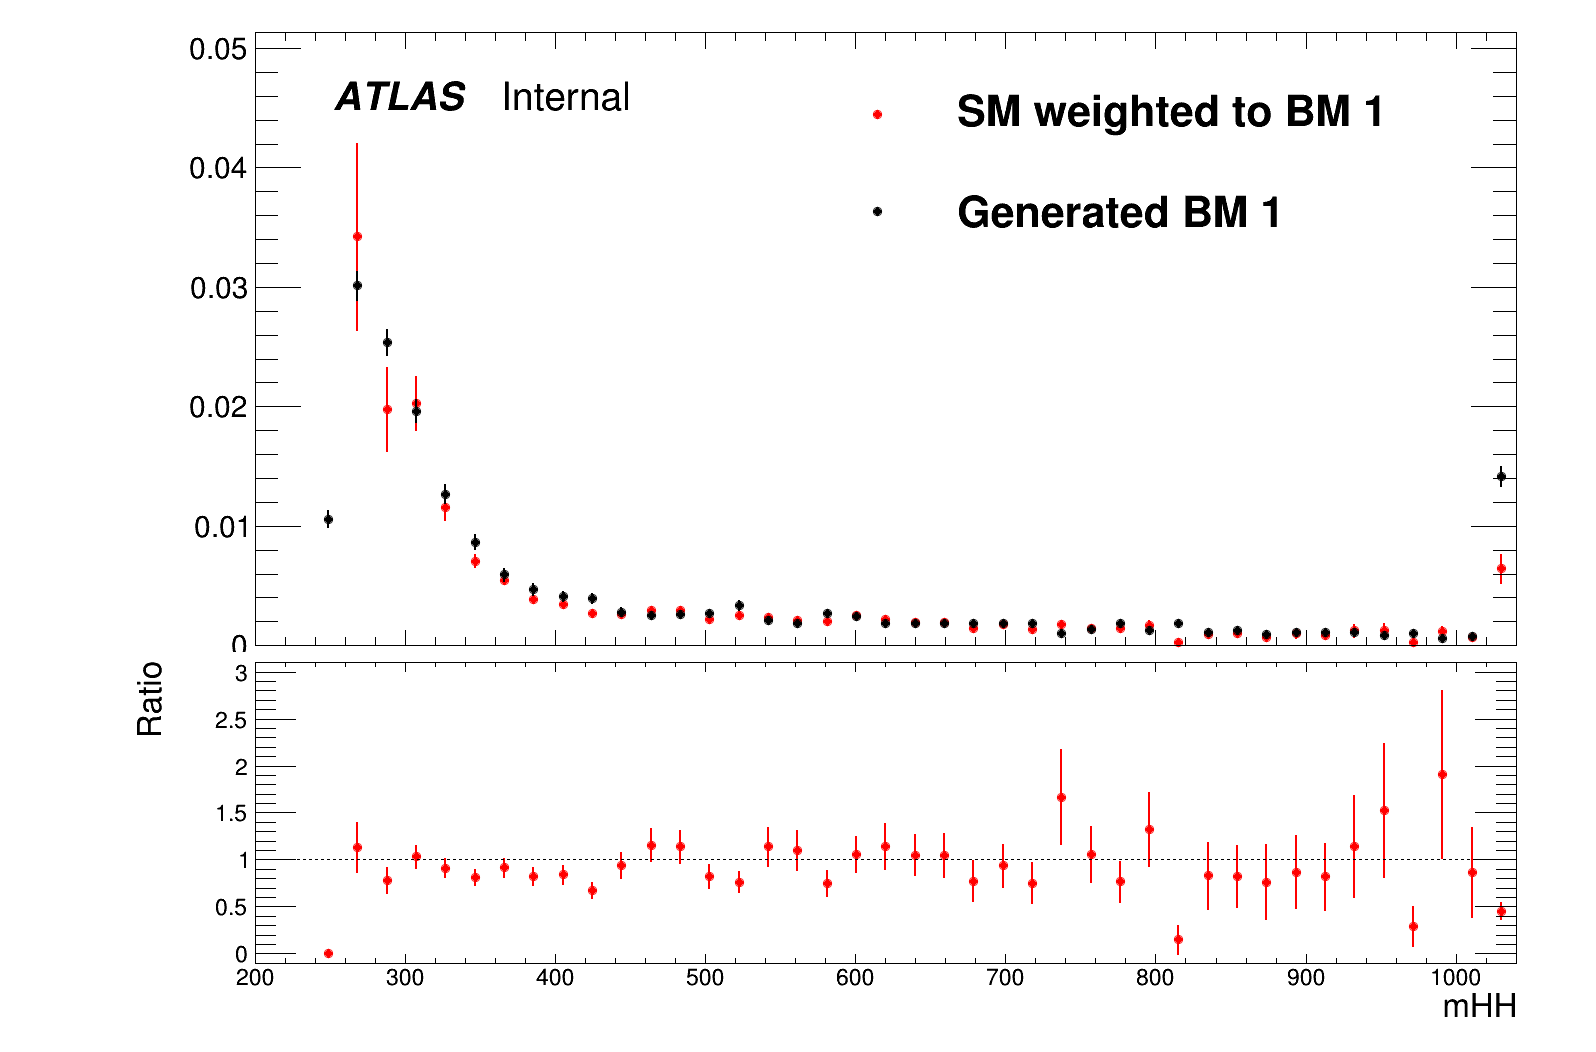
\includegraphics[width=.32\textwidth]{figures/Method_B_all_latest/BM1h_mHH.png}
    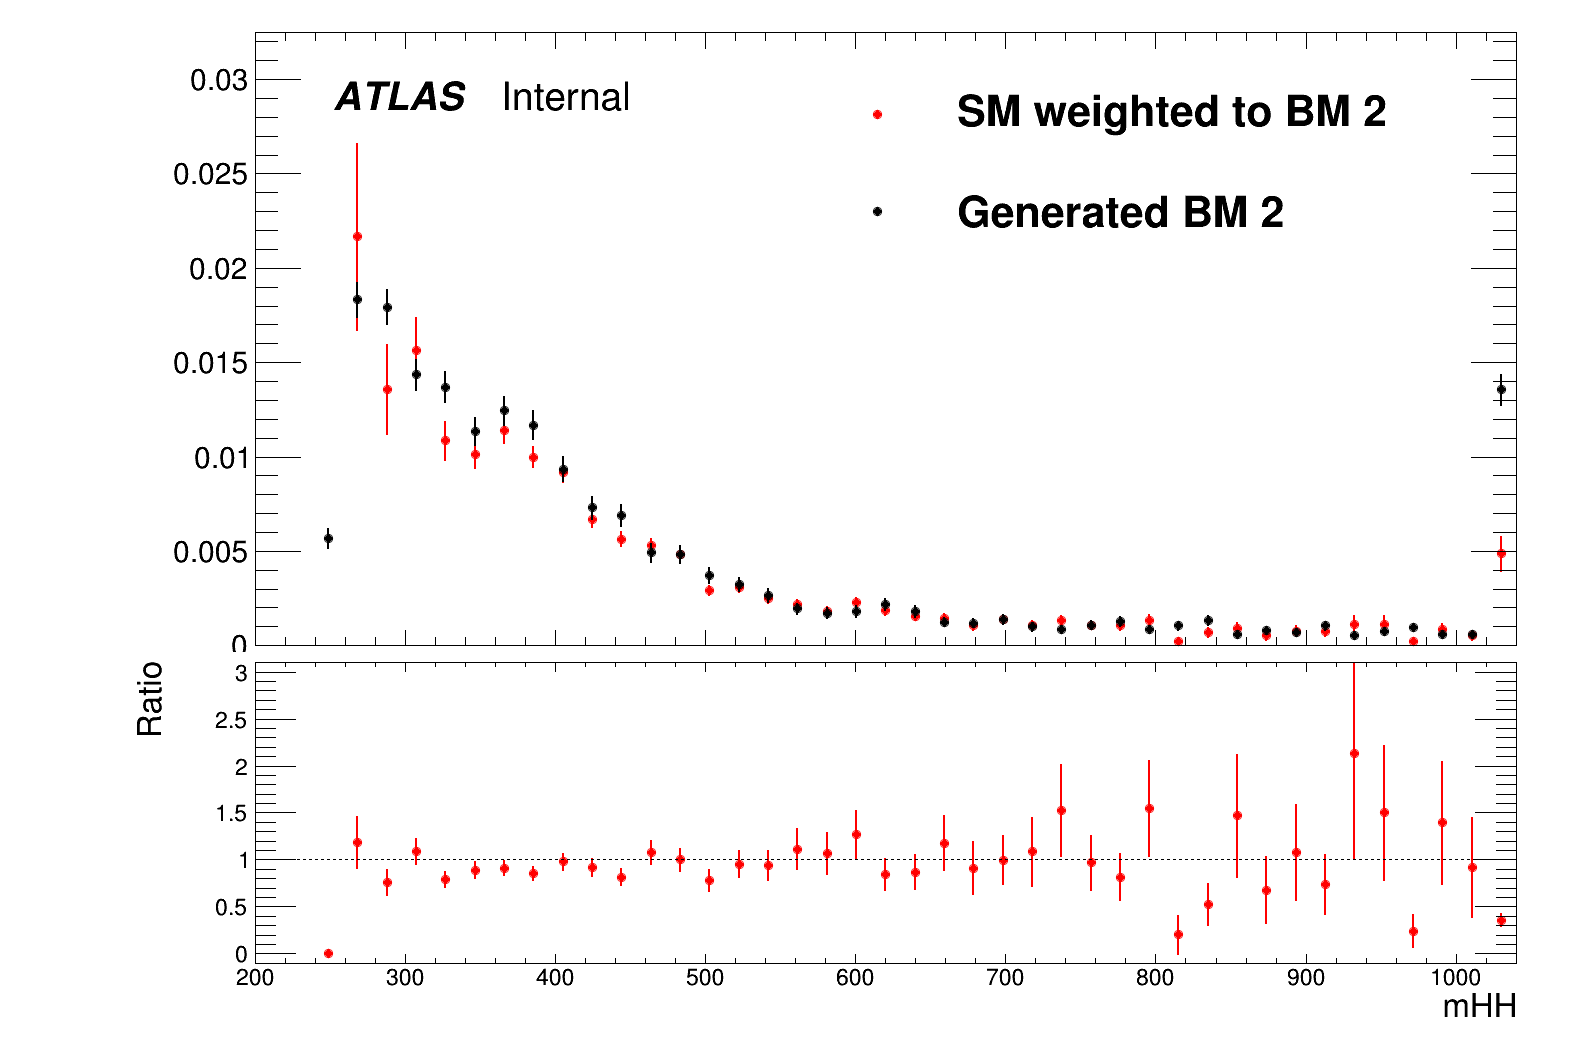
\includegraphics[width=.32\textwidth]{figures/Method_B_all_latest/BM2h_mHH.png}
    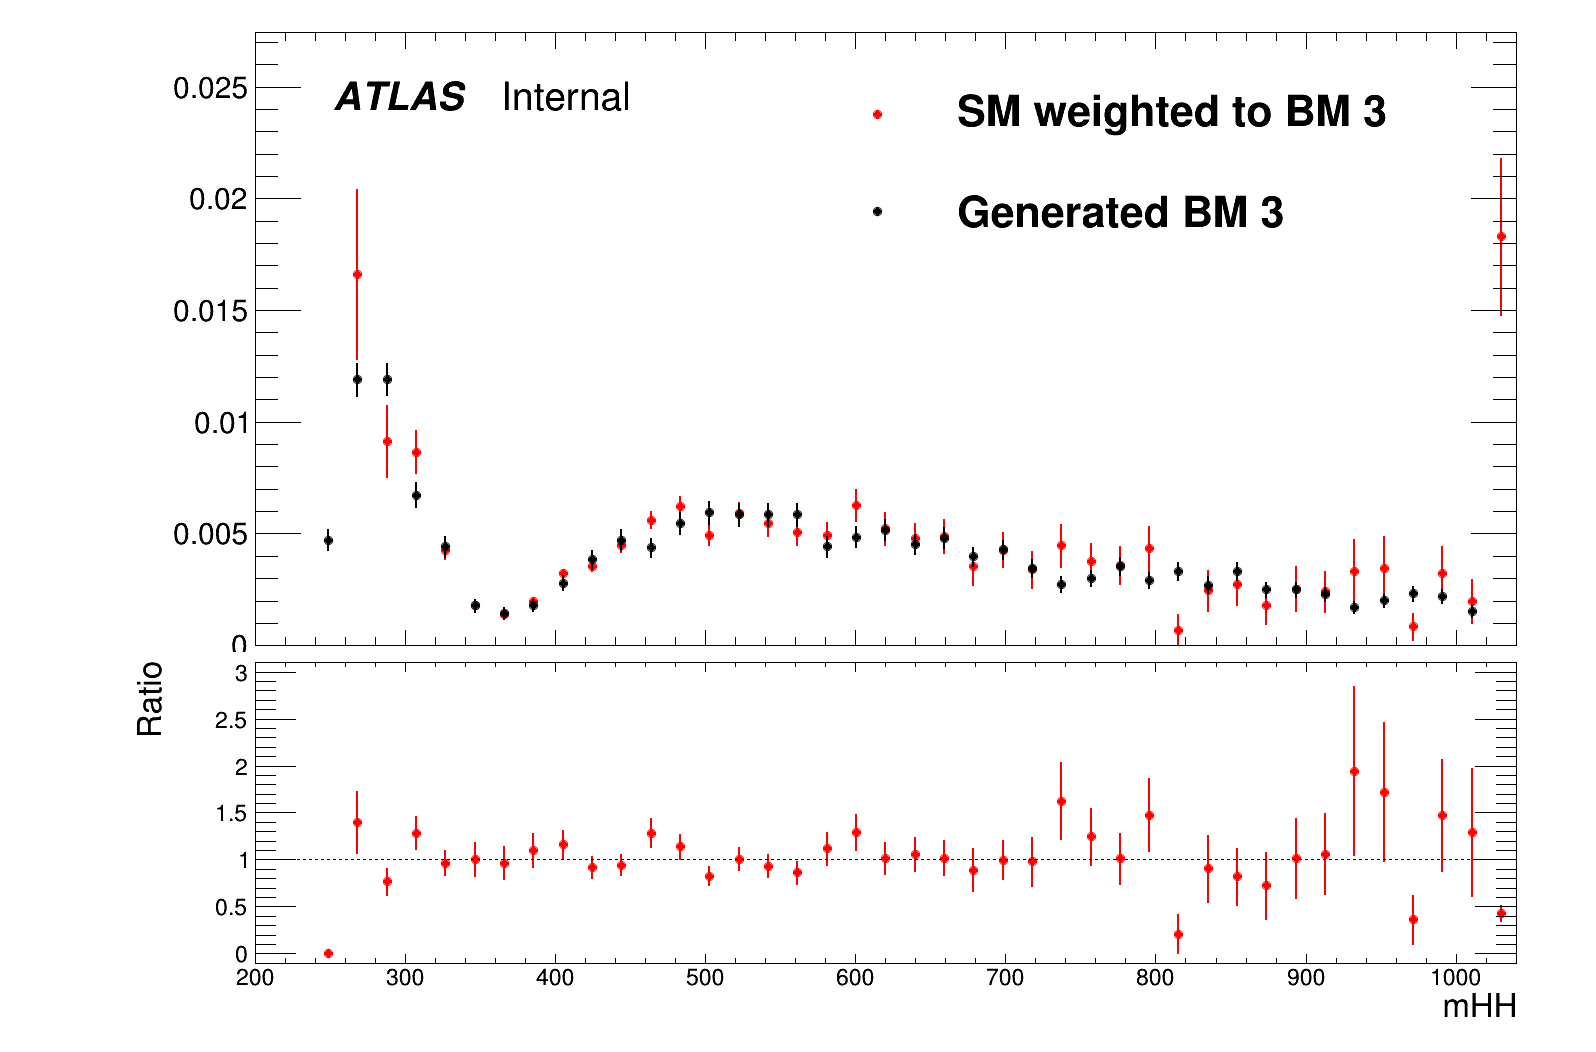
\includegraphics[width=.32\textwidth]{figures/Method_B_all_latest/BM3h_mHH.png}\\
    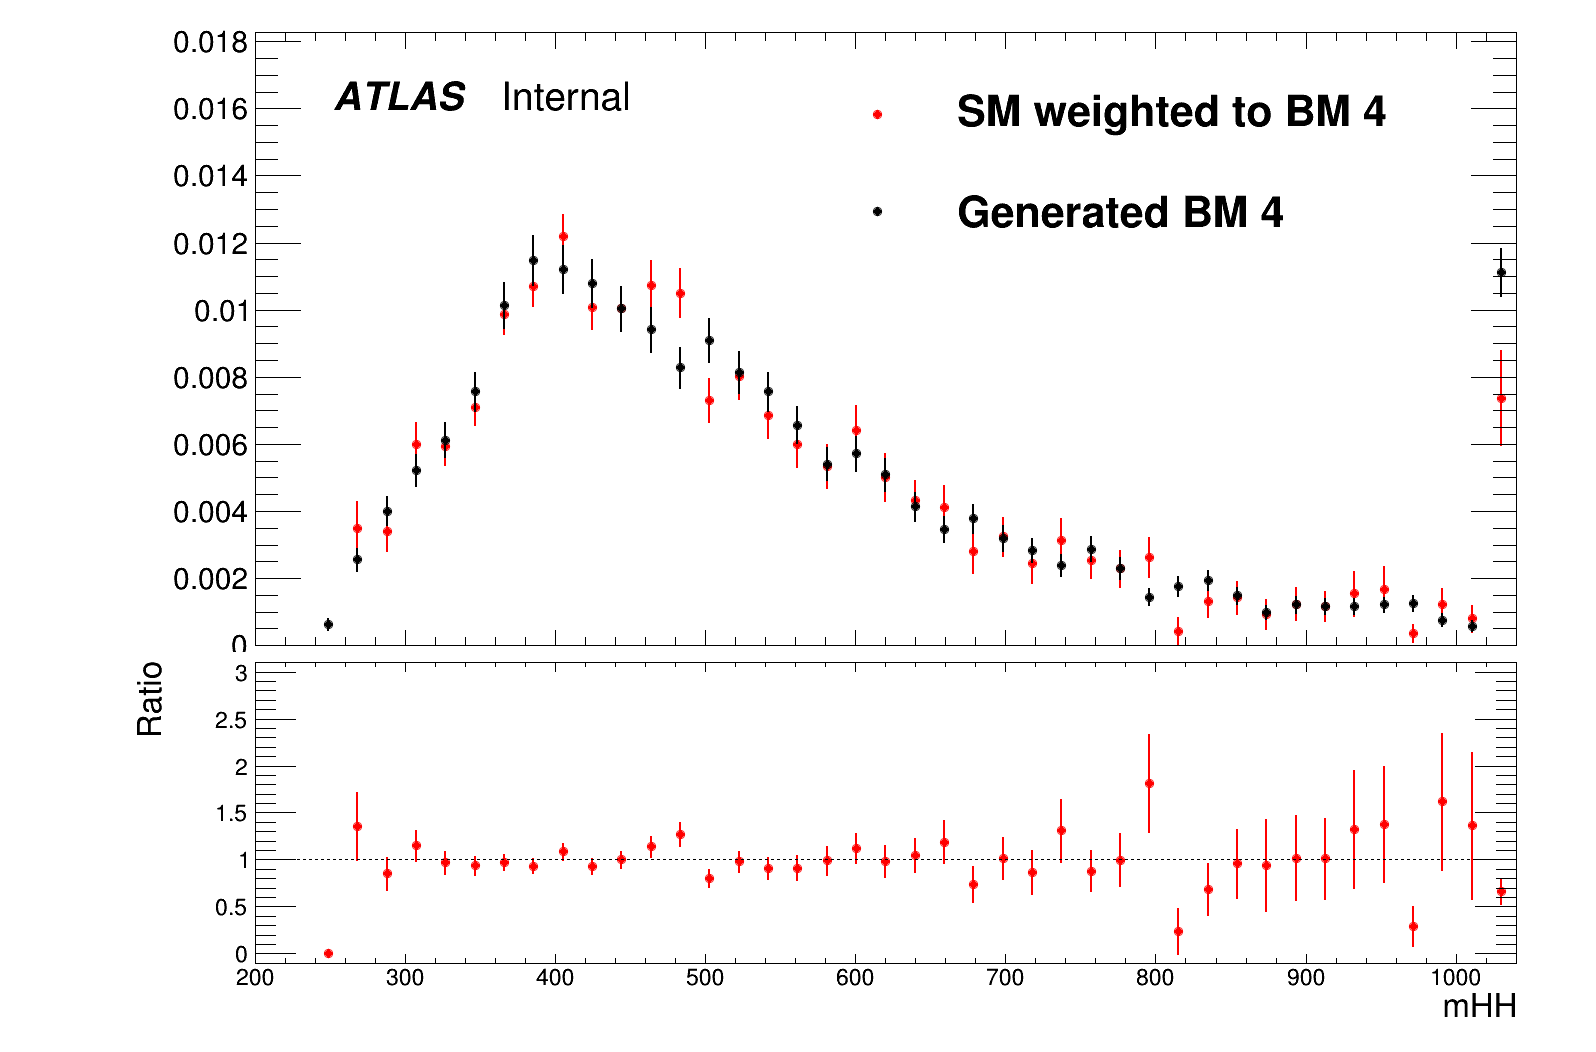
\includegraphics[width=.32\textwidth]{figures/Method_B_all_latest/BM4h_mHH.png}
    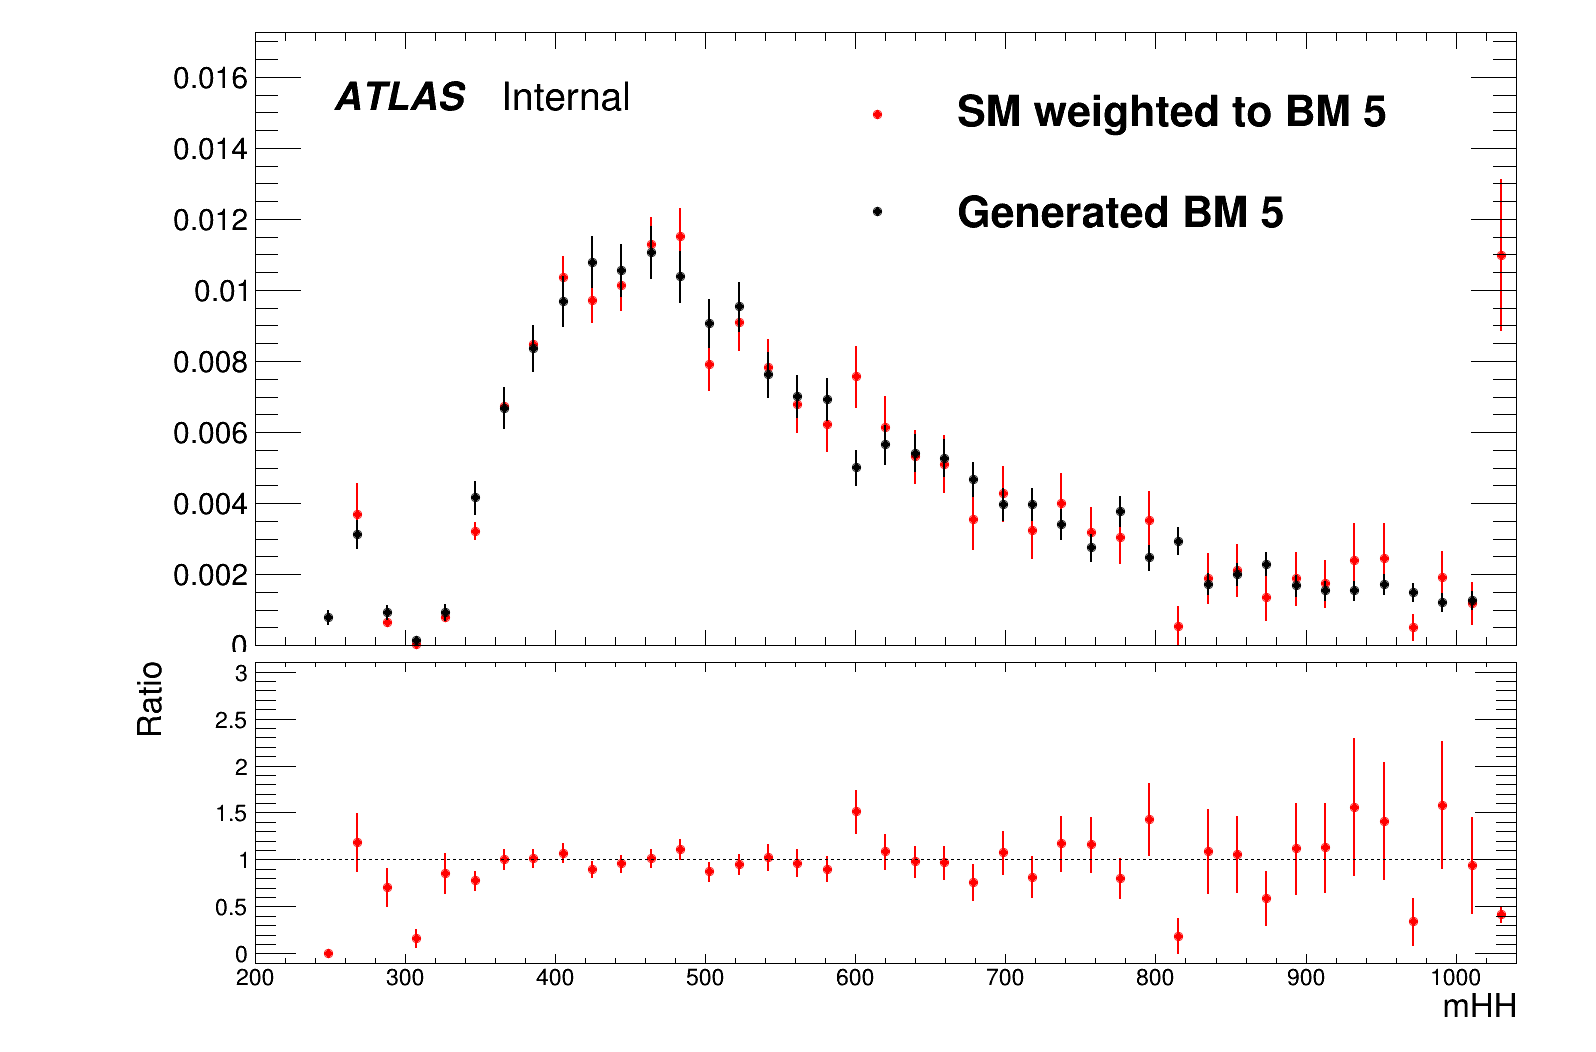
\includegraphics[width=.32\textwidth]{figures/Method_B_all_latest/BM5h_mHH.png}
    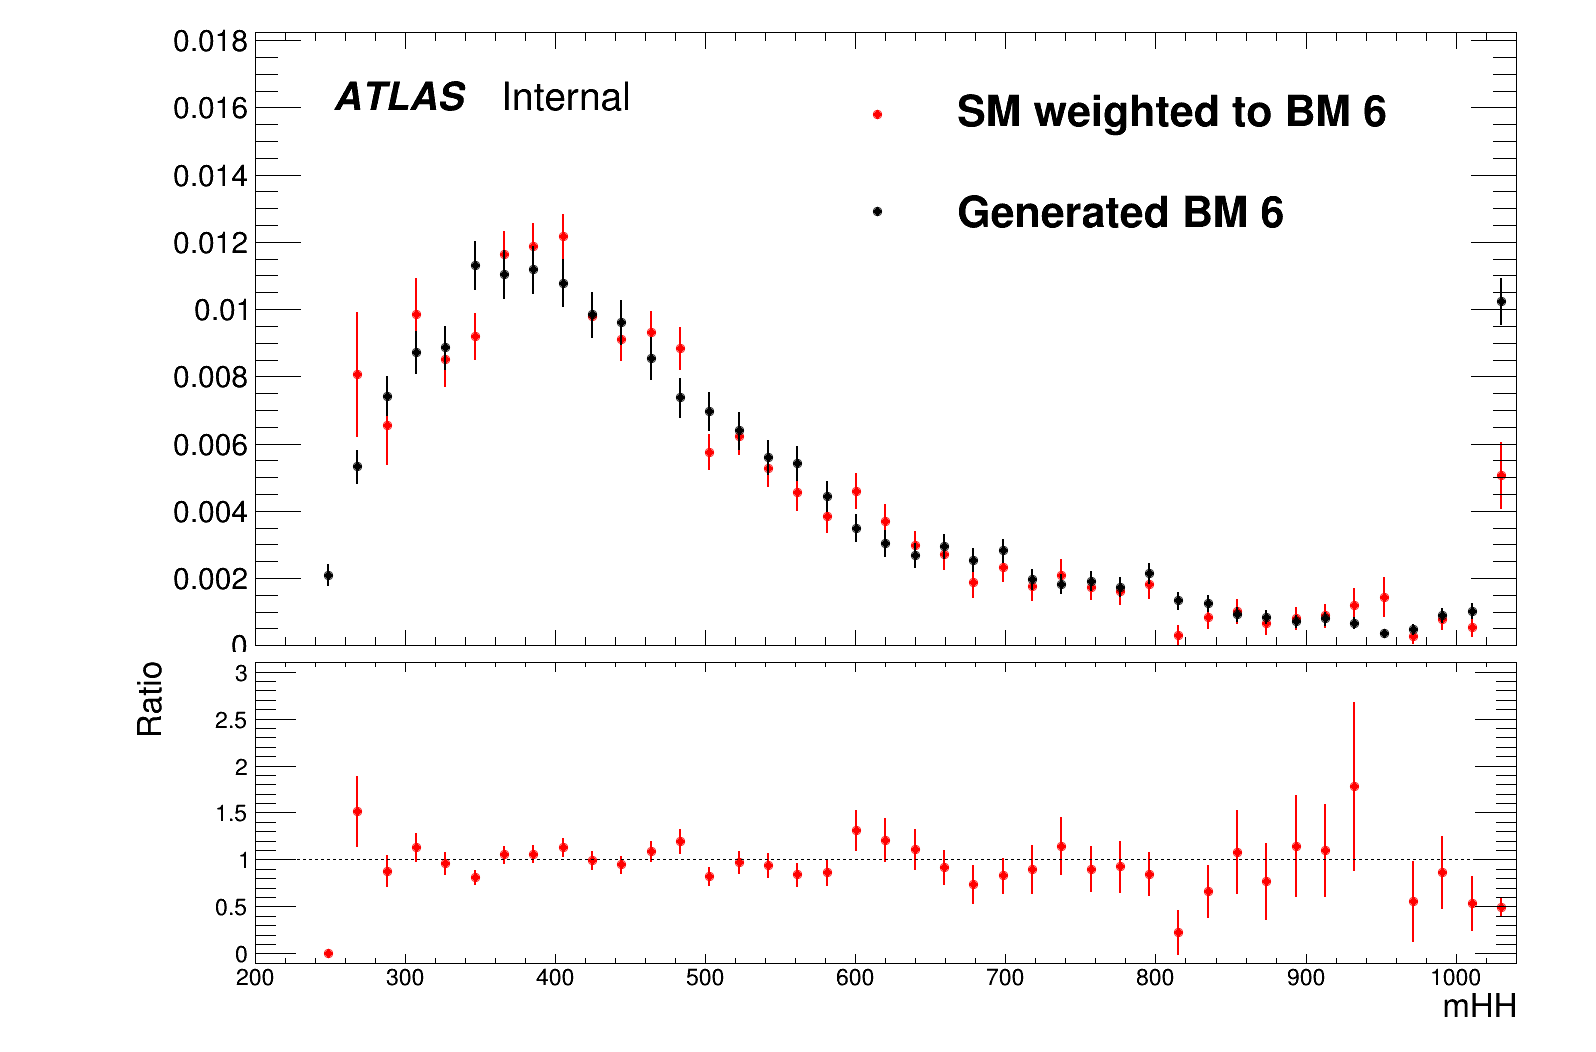
\includegraphics[width=.32\textwidth]{figures/Method_B_all_latest/BM6h_mHH.png}\\
    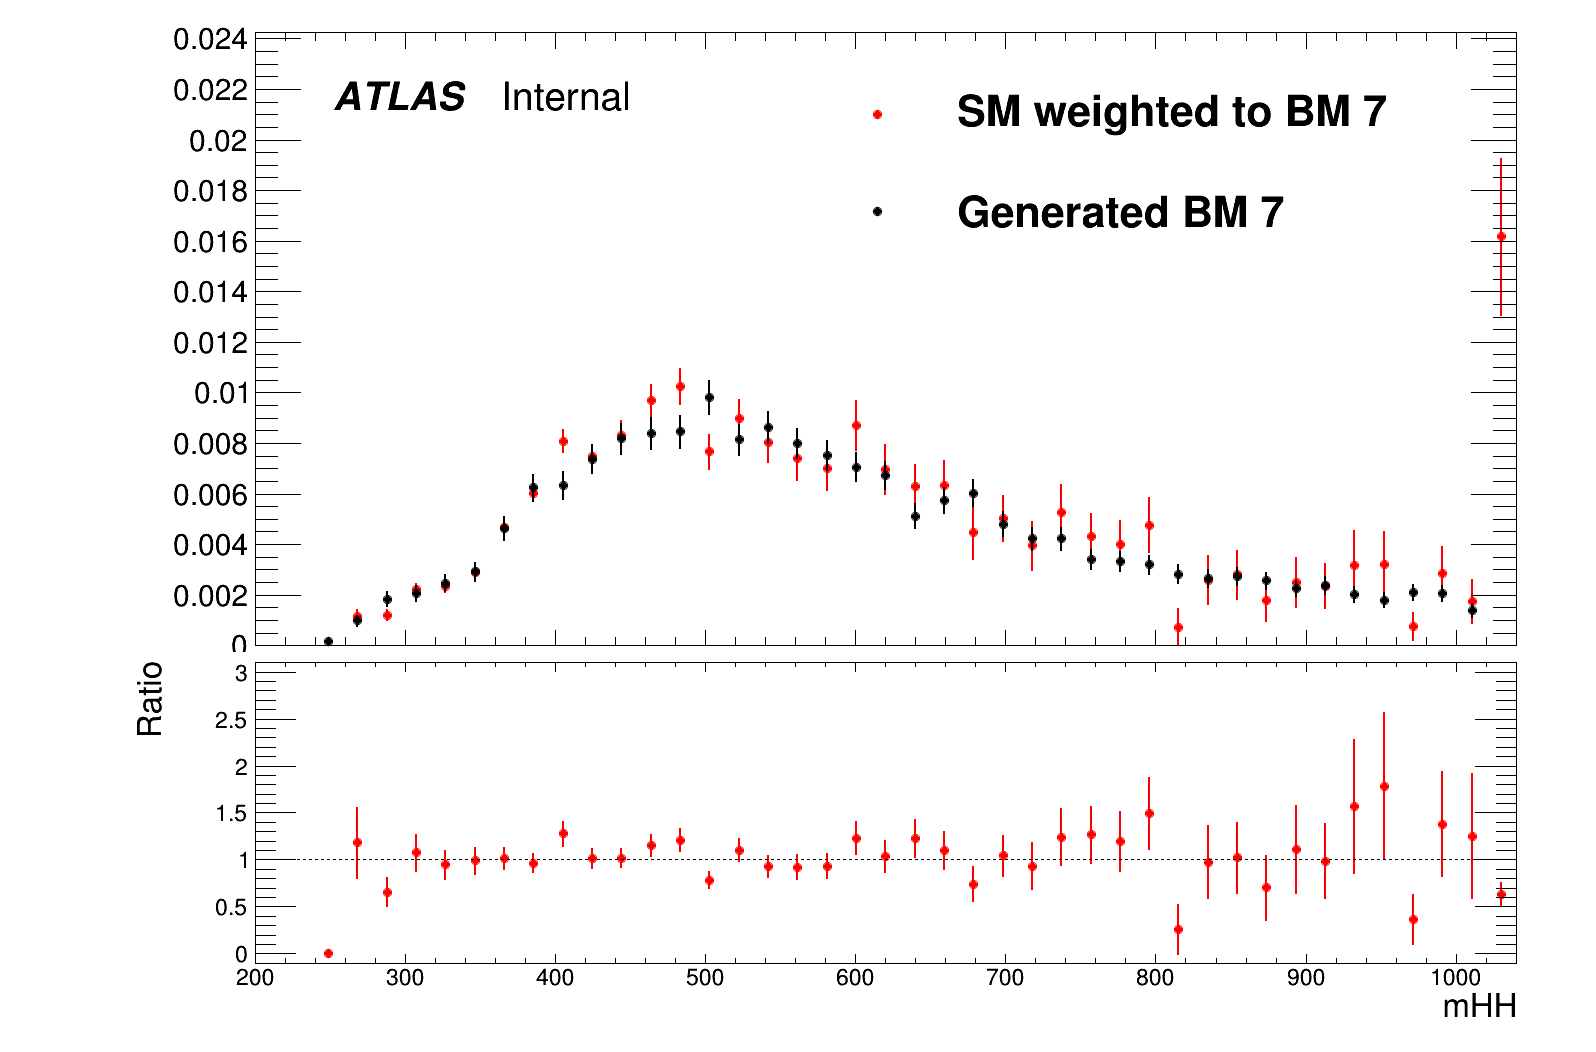
\includegraphics[width=.32\textwidth]{figures/Method_B_all_latest/BM7h_mHH.png}

\end{frame}

\begin{frame}
    \frametitle{SLT $c_{ggHH}$ scan $\Delta R_{\tau\tau}$ shape: weighted SM vs generated BM}

    \begin{figure}
    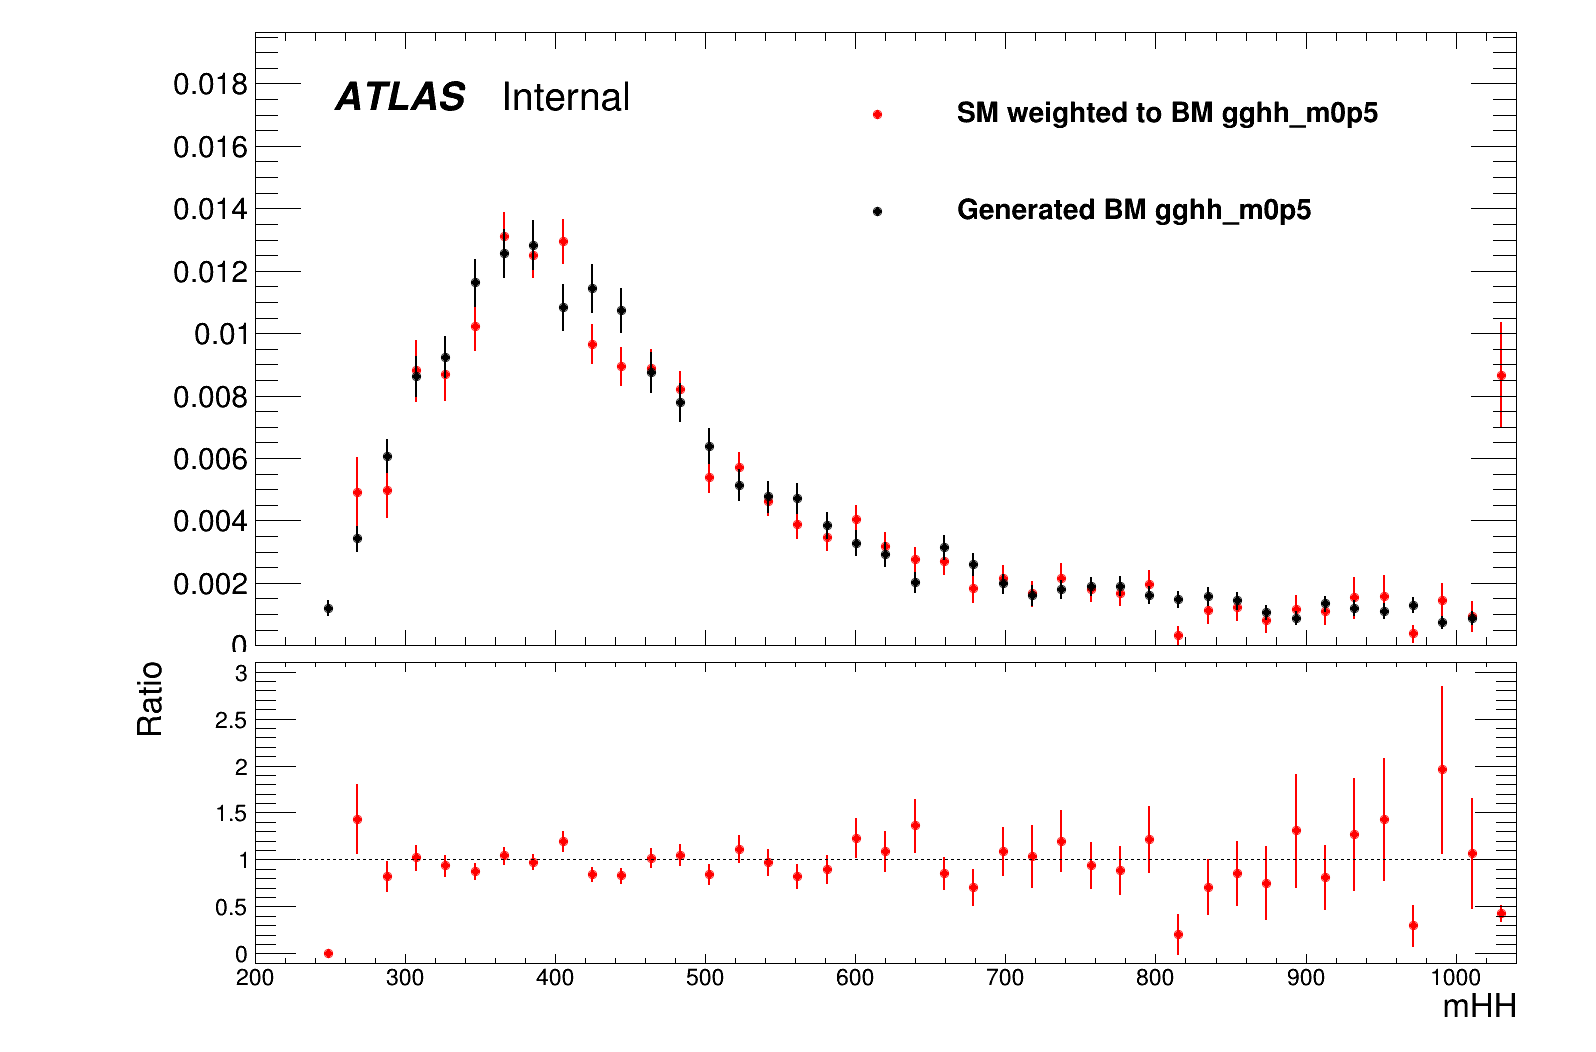
\includegraphics[width=.32\textwidth]{figures/Method_B_all_latest/BMgghh_m0p5h_mHH.png}
    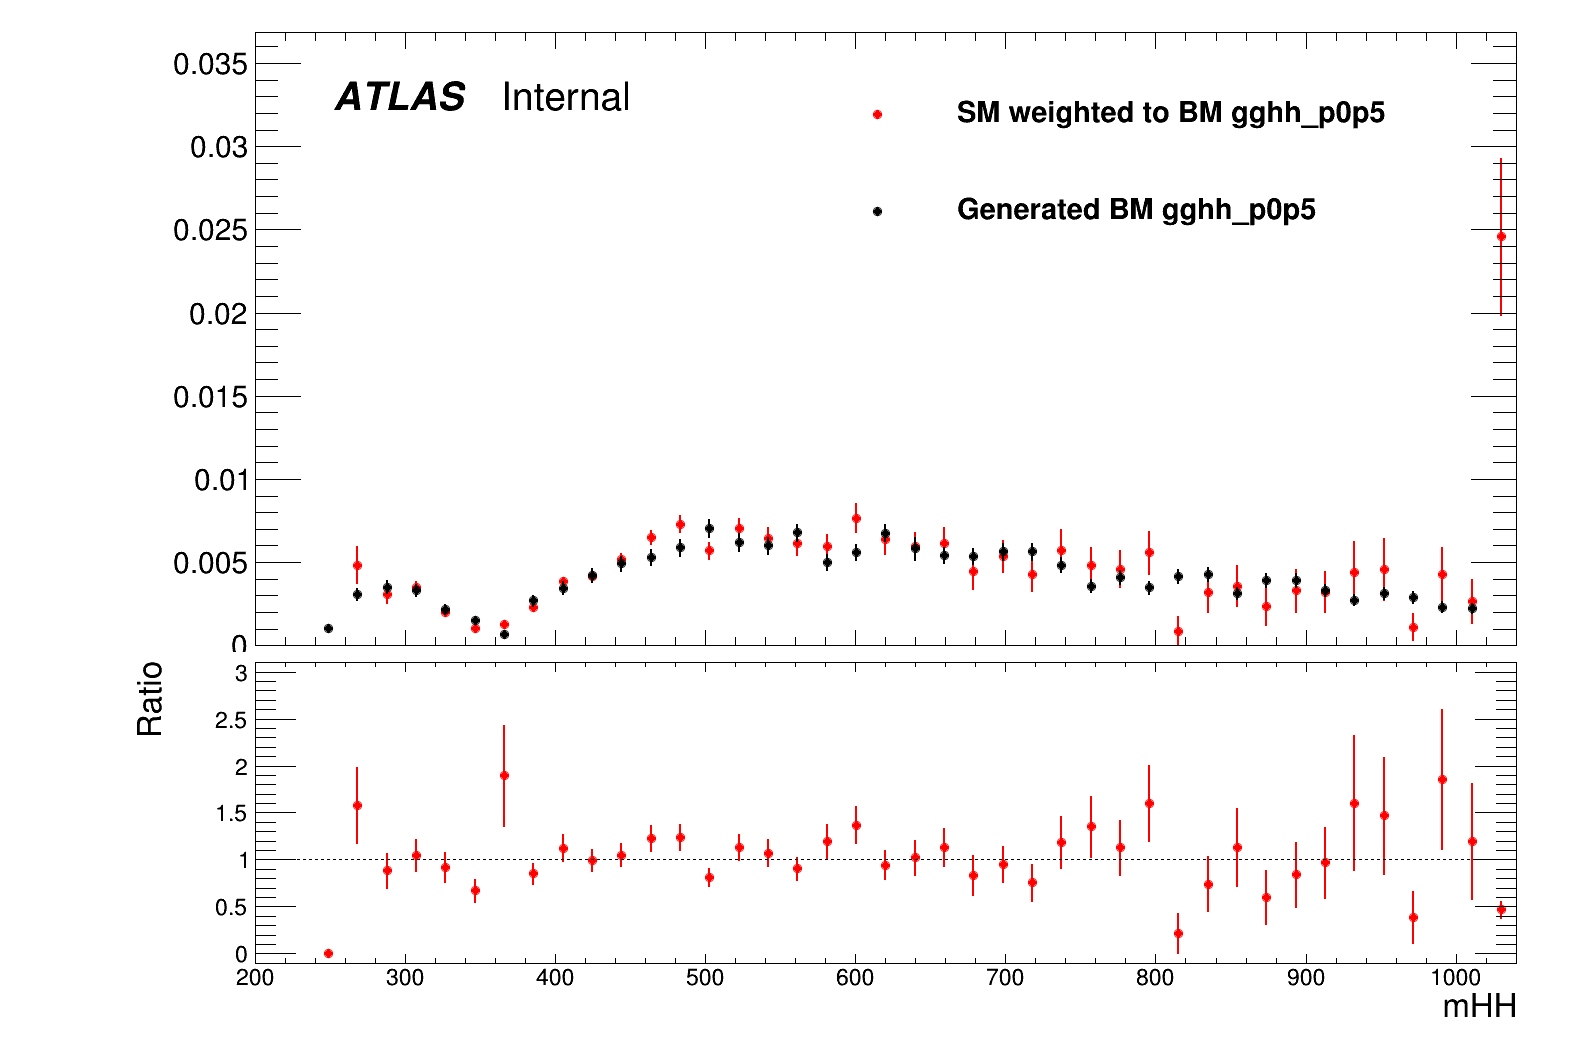
\includegraphics[width=.32\textwidth]{figures/Method_B_all_latest/BMgghh_p0p5h_mHH.png}
    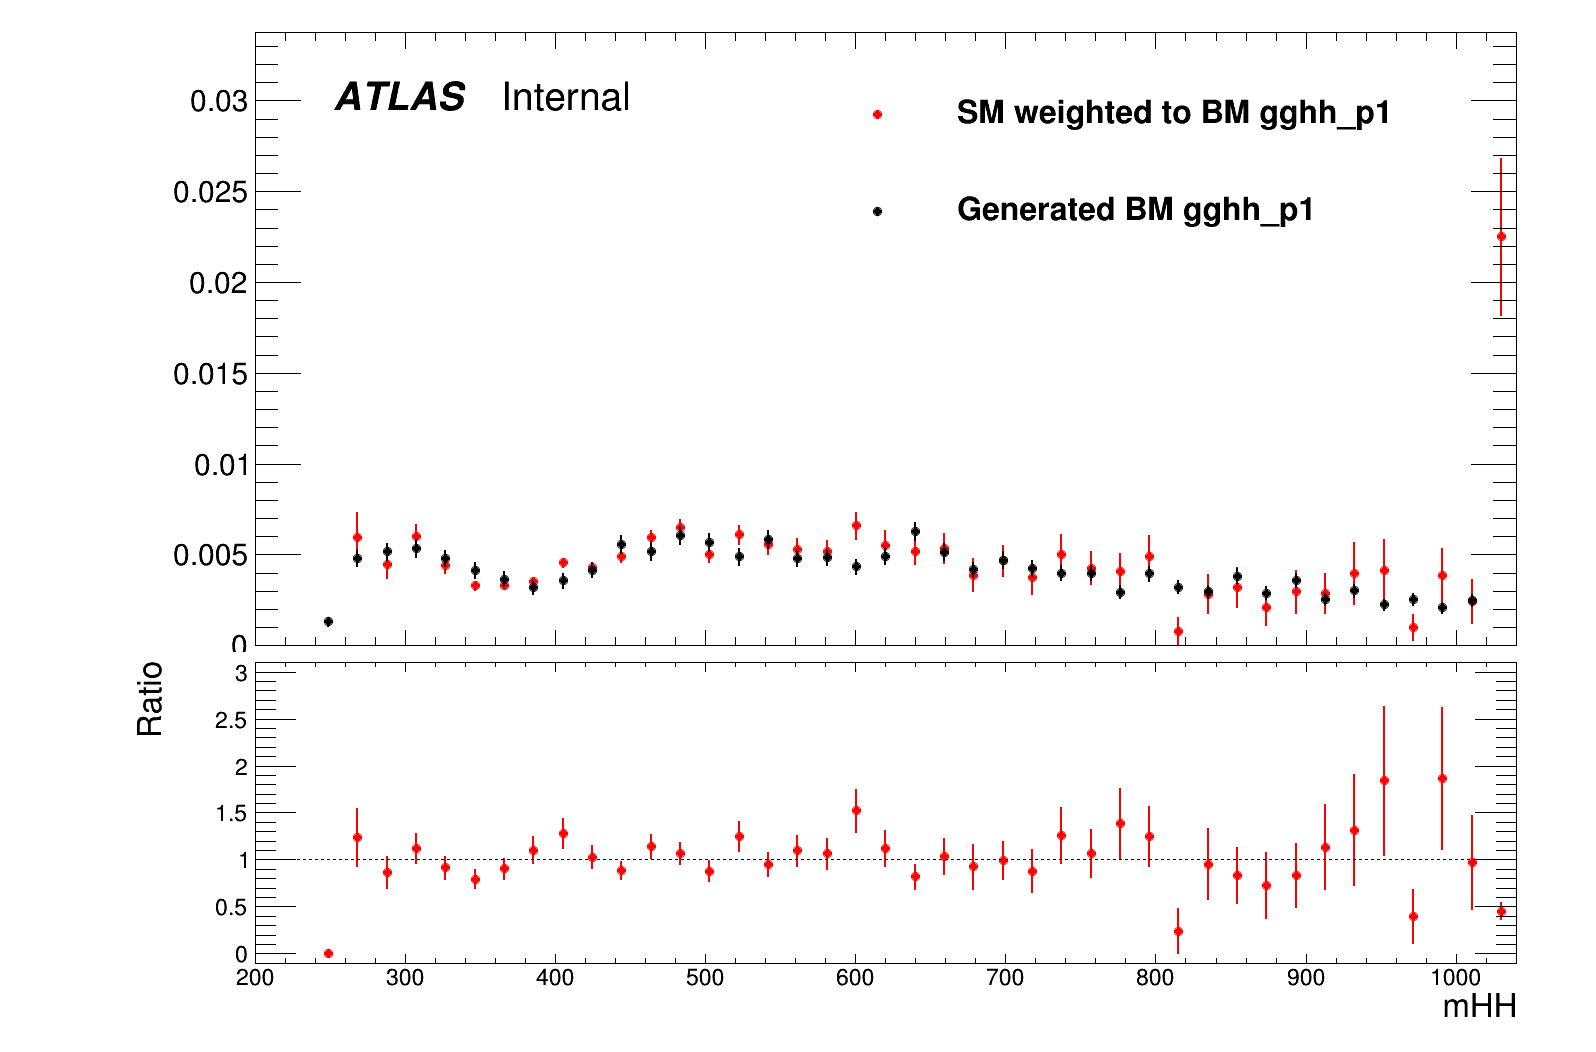
\includegraphics[width=.32\textwidth]{figures/Method_B_all_latest/BMgghh_p1h_mHH.png}
    $c_{ggHH} = -0.5$ \hspace{5em} $c_{ggHH} = 0.5$\hspace{5em} $c_{ggHH} = 1.0$
    \end{figure}


\end{frame}     

\begin{frame}
    \frametitle{SLT $c_{ttHH}$ scan $\Delta R_{\tau\tau}$ shape: weighted SM vs generated BM}
\begin{figure}
    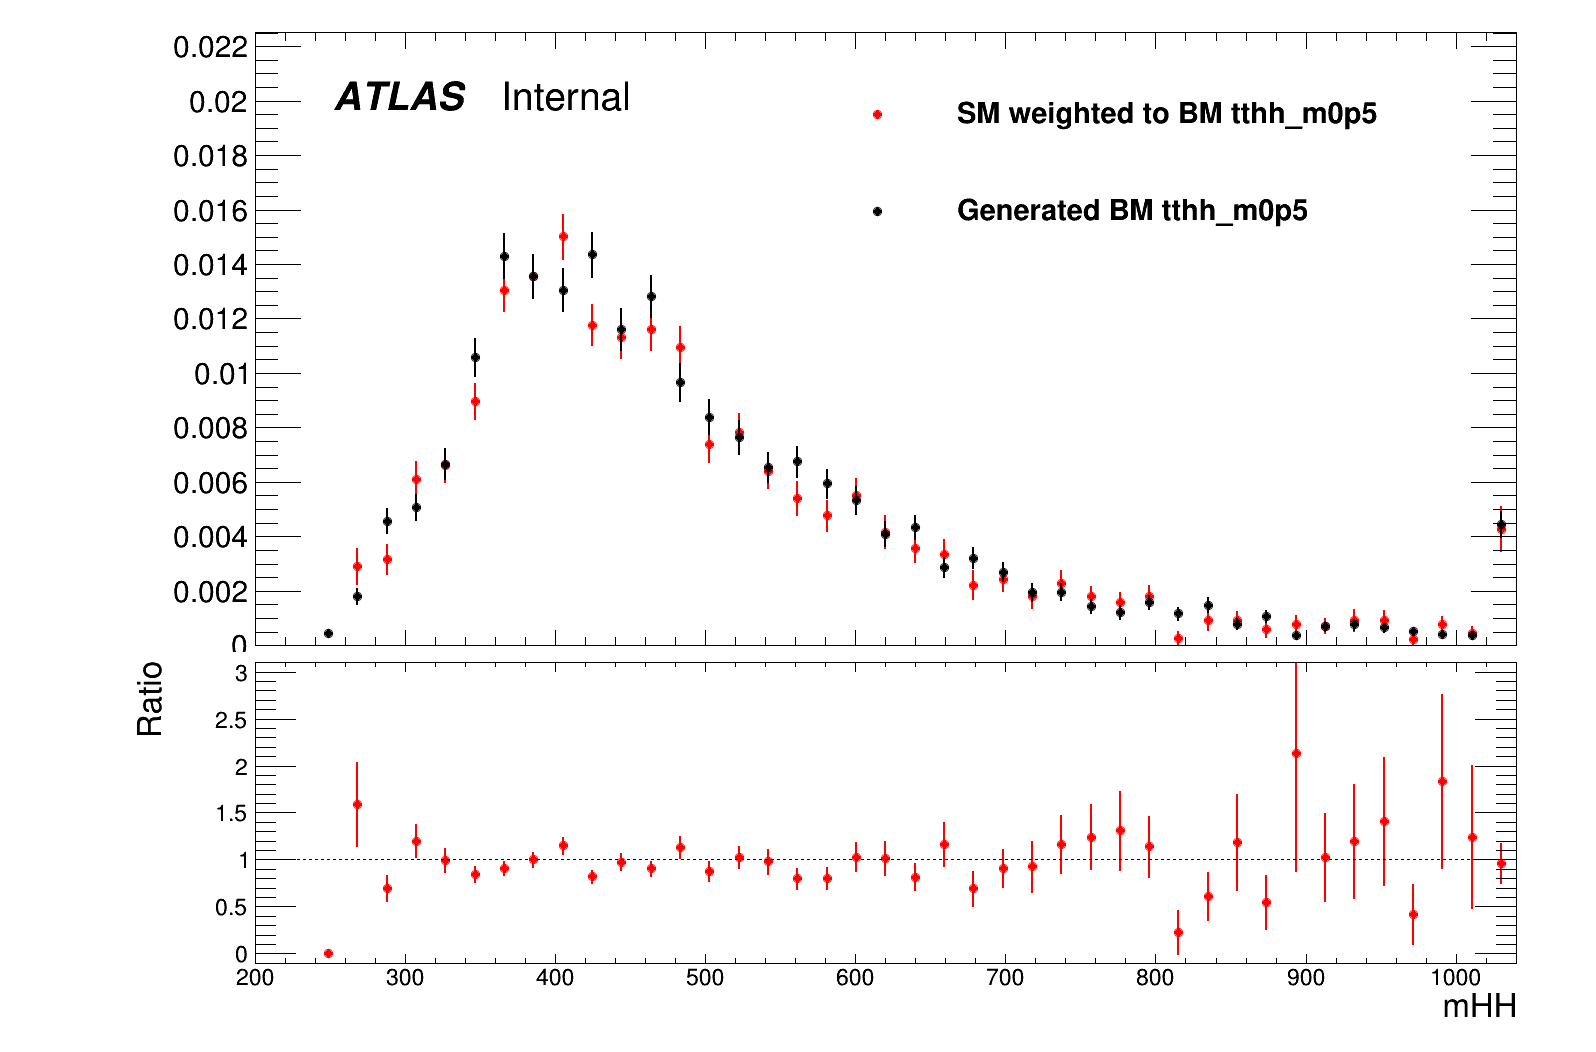
\includegraphics[width=.32\textwidth]{figures/Method_B_all_latest/BMtthh_m0p5h_mHH.png}
    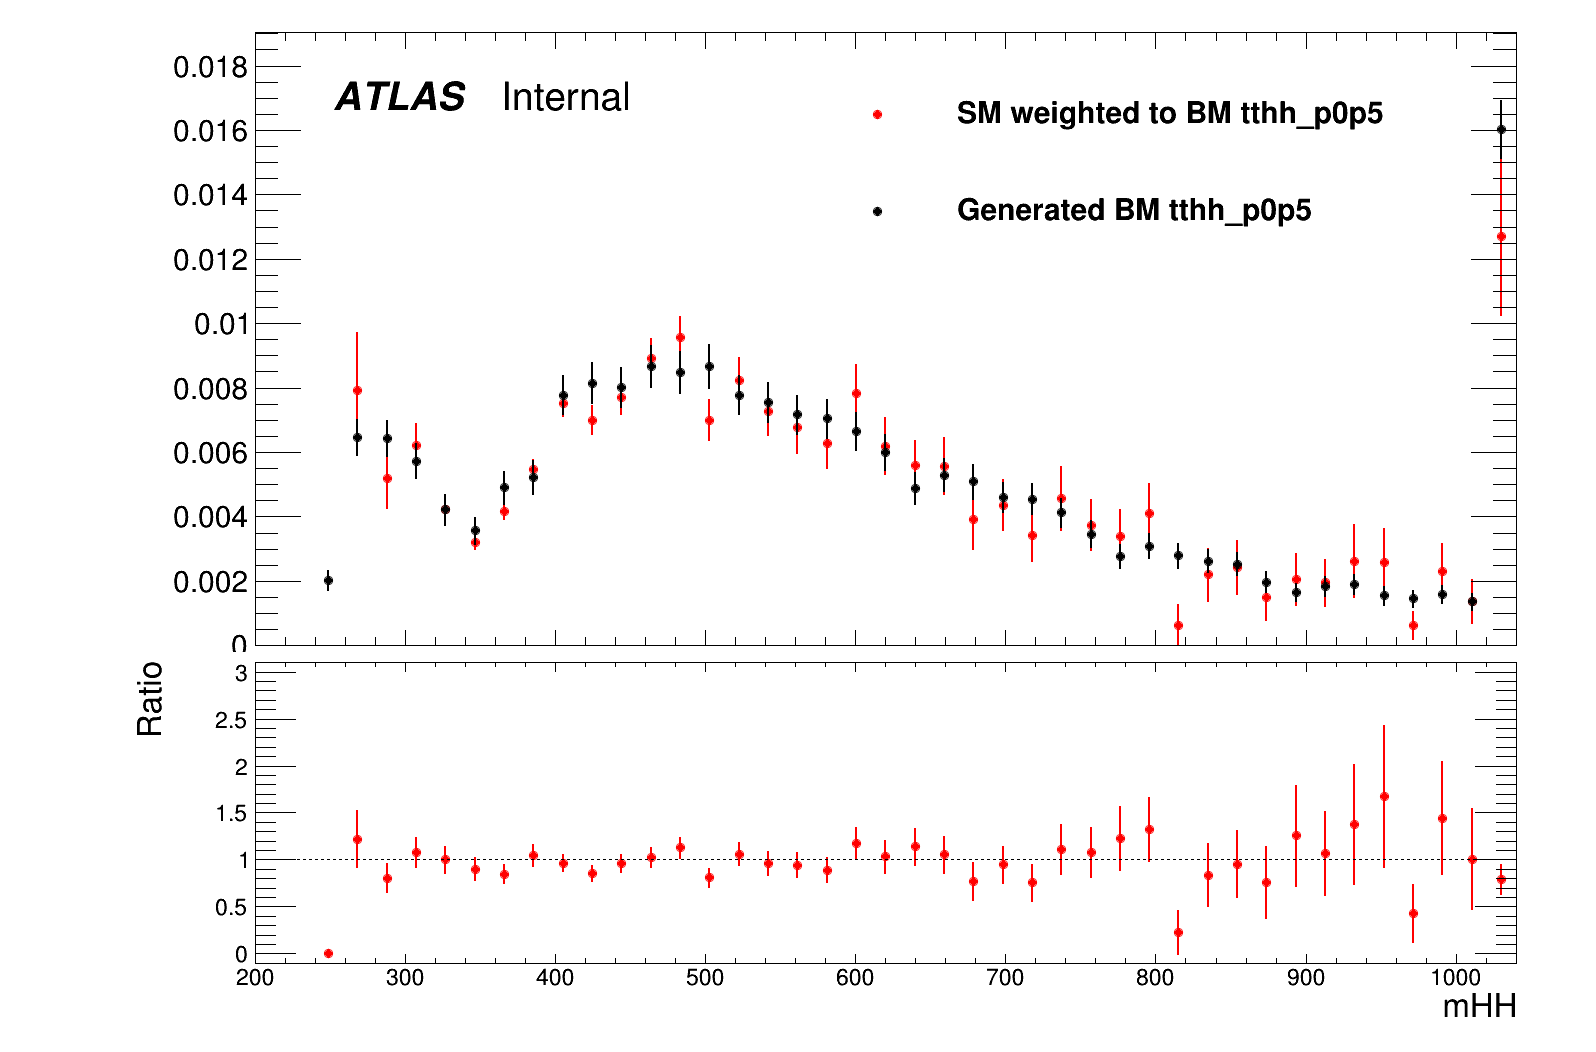
\includegraphics[width=.32\textwidth]{figures/Method_B_all_latest/BMtthh_p0p5h_mHH.png}
    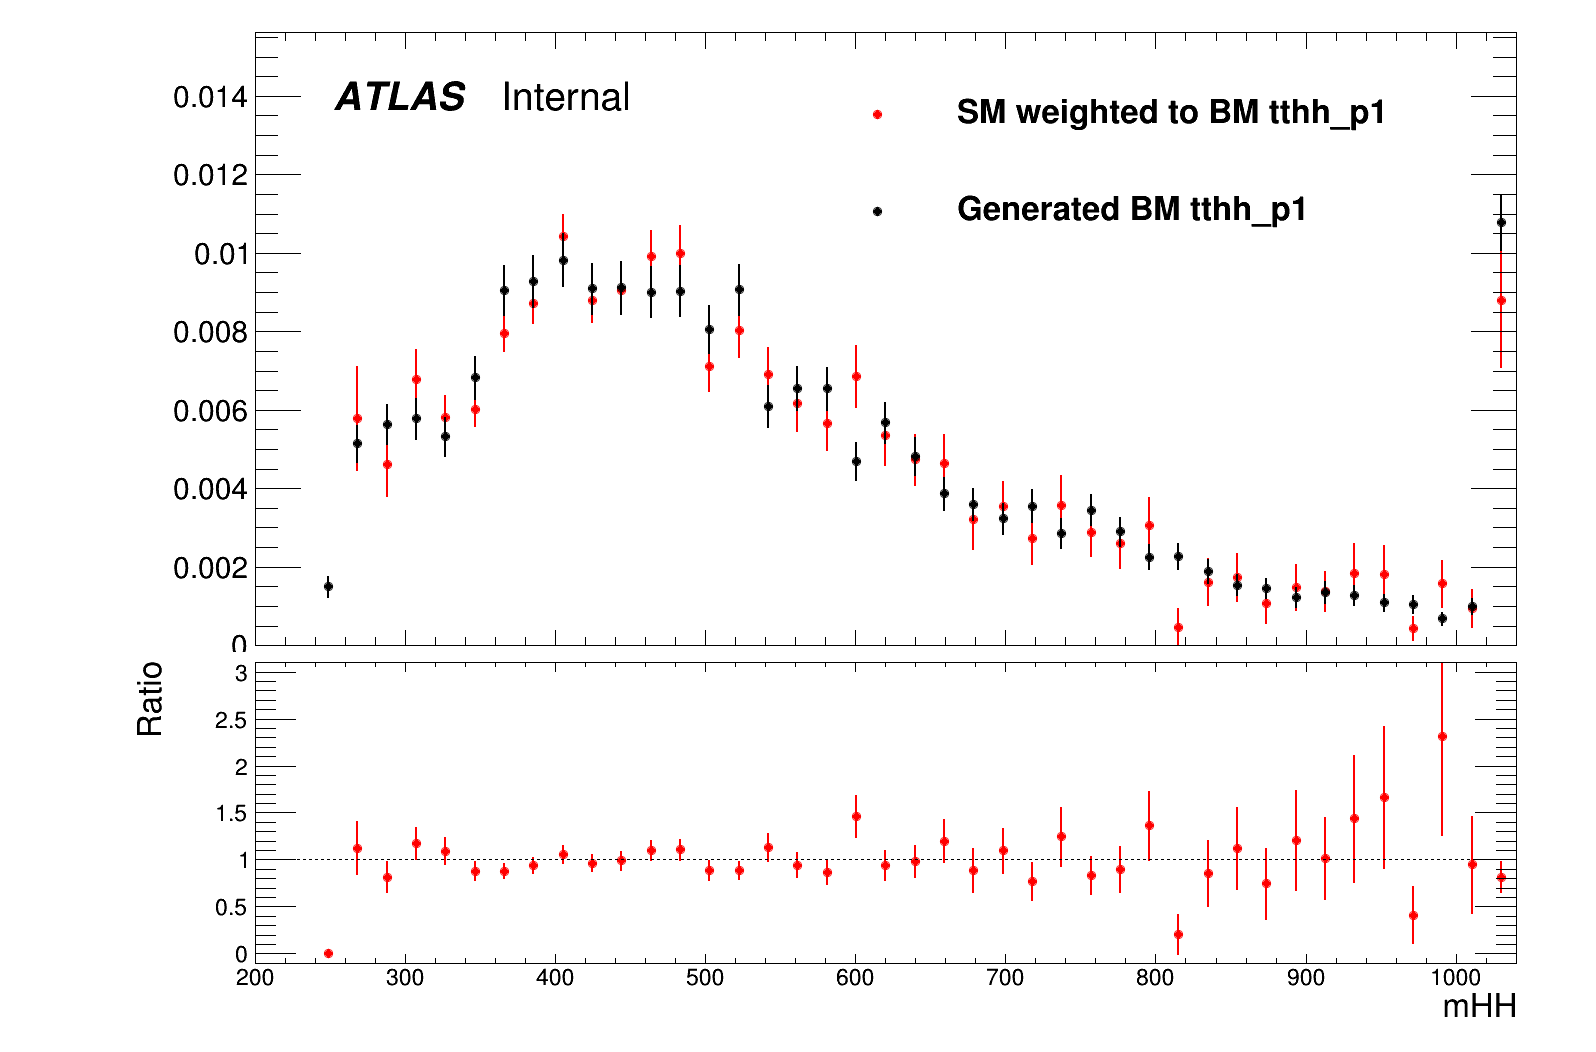
\includegraphics[width=.32\textwidth]{figures/Method_B_all_latest/BMtthh_p1h_mHH.png}
    $c_{ttHH} = -0.5$ \hspace{5em} $c_{ttHH} = 0.5$\hspace{5em} $c_{ttHH} = 1.0$    
\end{figure}

\end{frame}   




\begin{frame}
    \frametitle{LTT BMs $\Delta R_{\tau\tau}$ shape: weighted SM vs generated BM}
\centering  
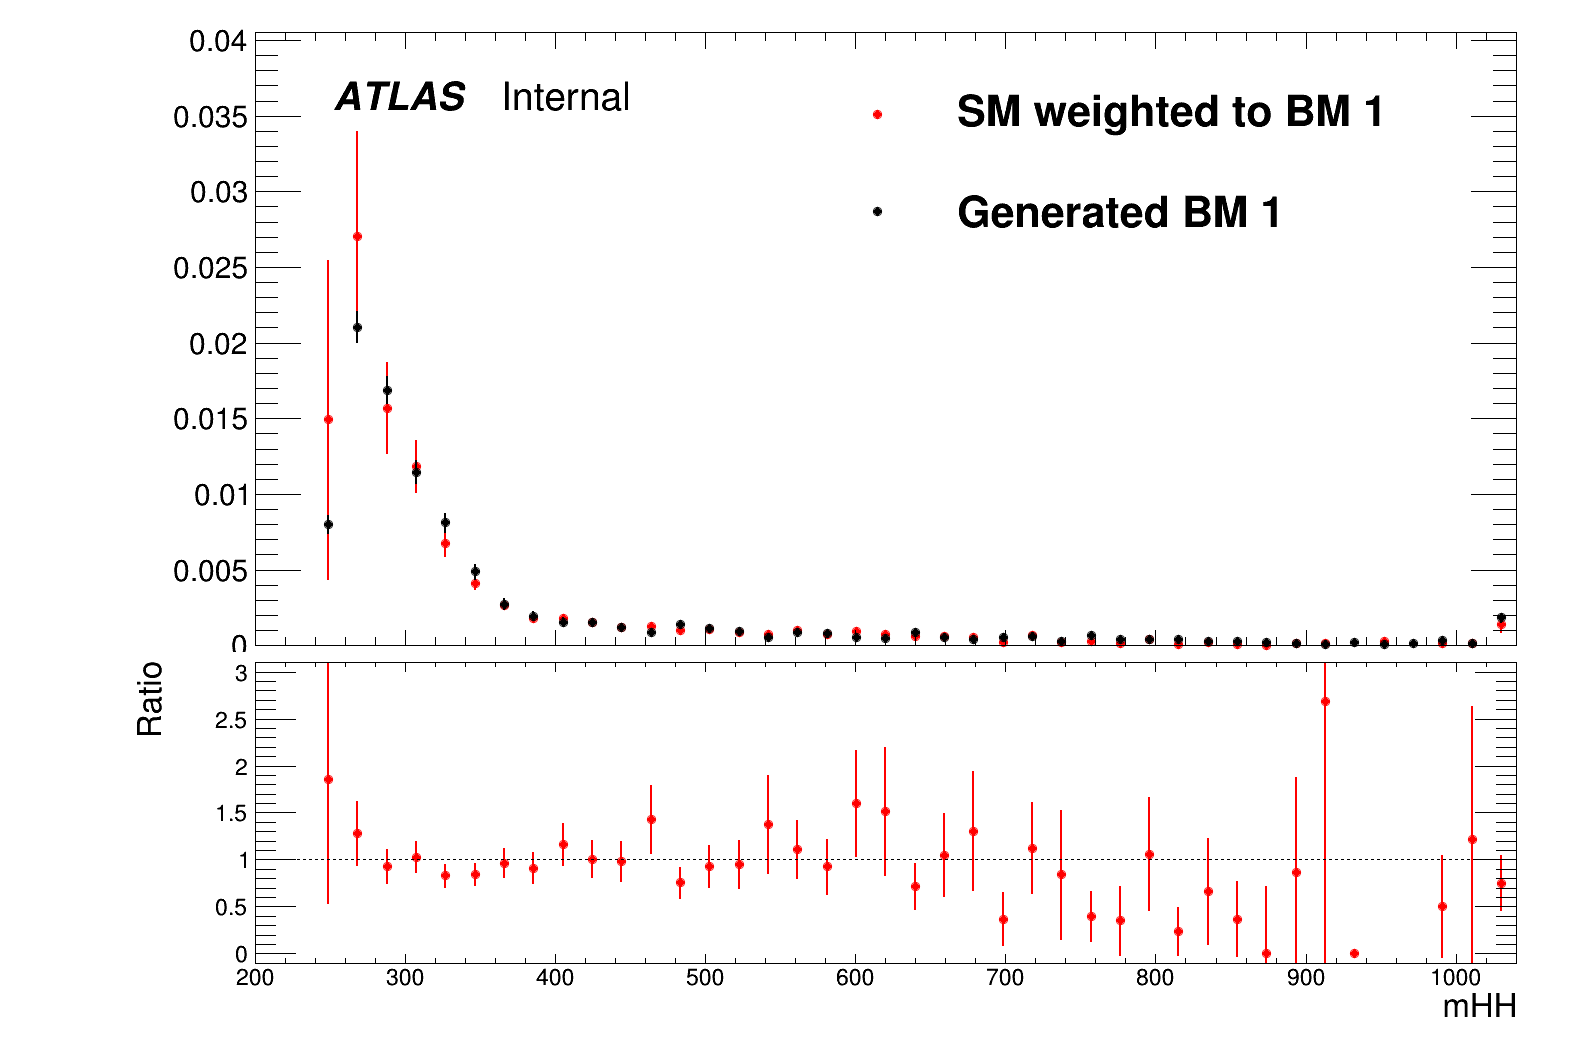
\includegraphics[width=.32\textwidth]{figures/Method_B_all_latest_LTT/BM1h_mHH.png}
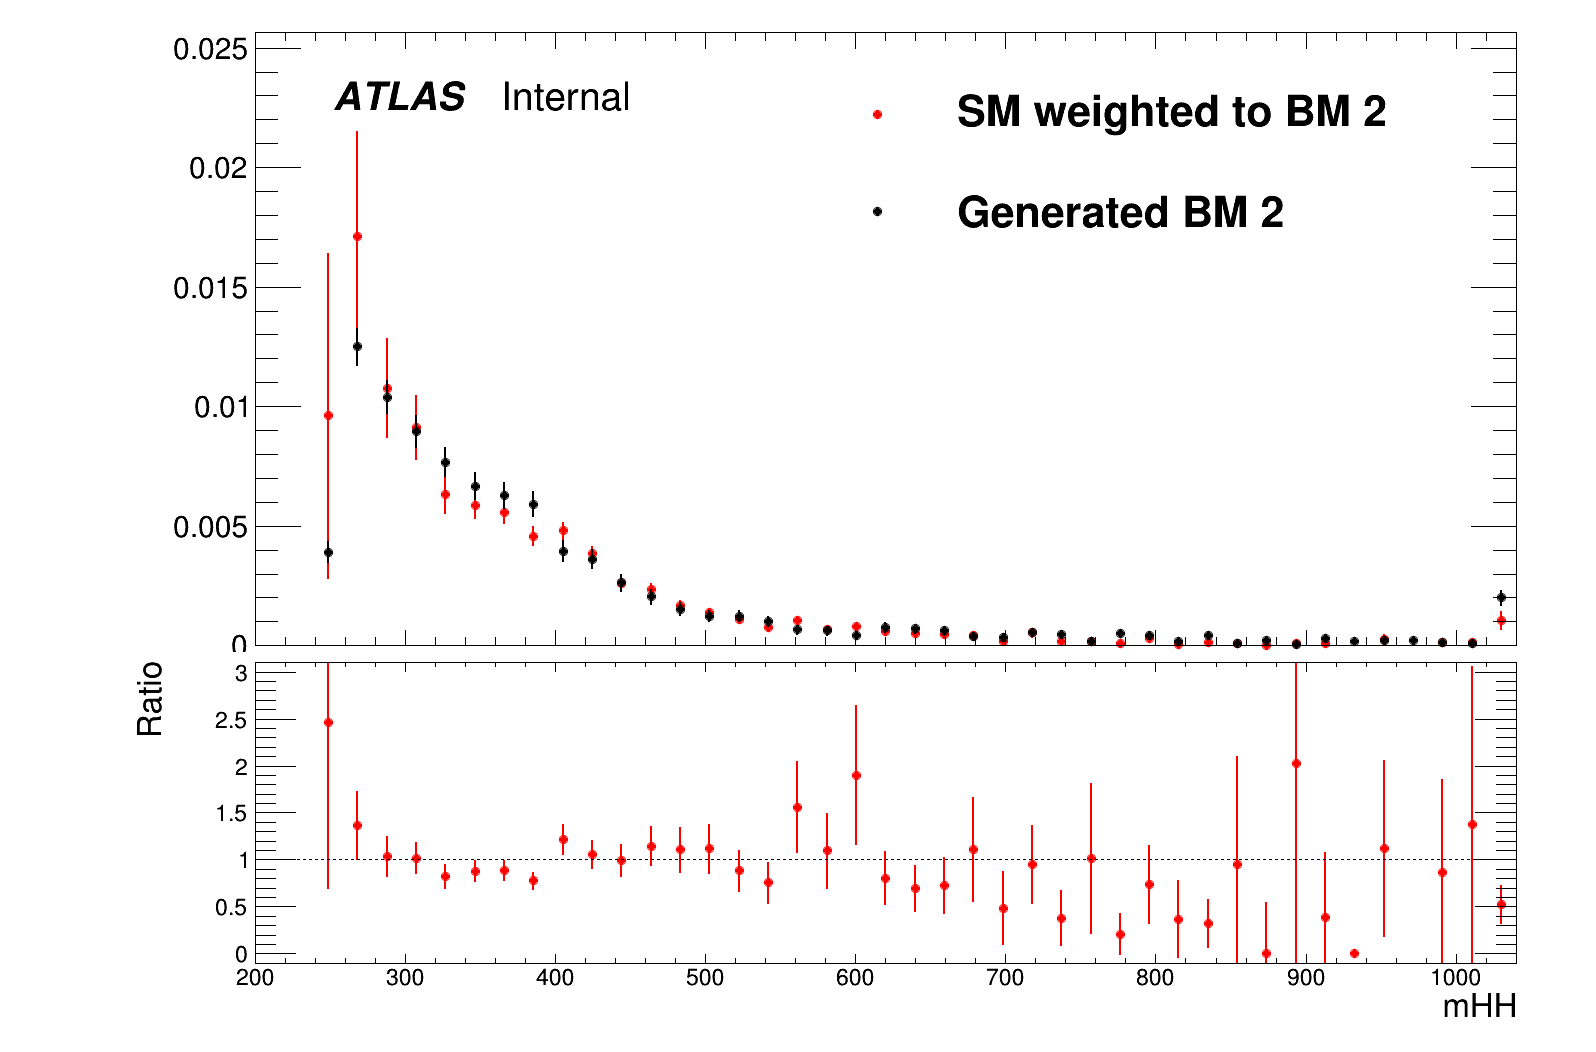
\includegraphics[width=.32\textwidth]{figures/Method_B_all_latest_LTT/BM2h_mHH.png}
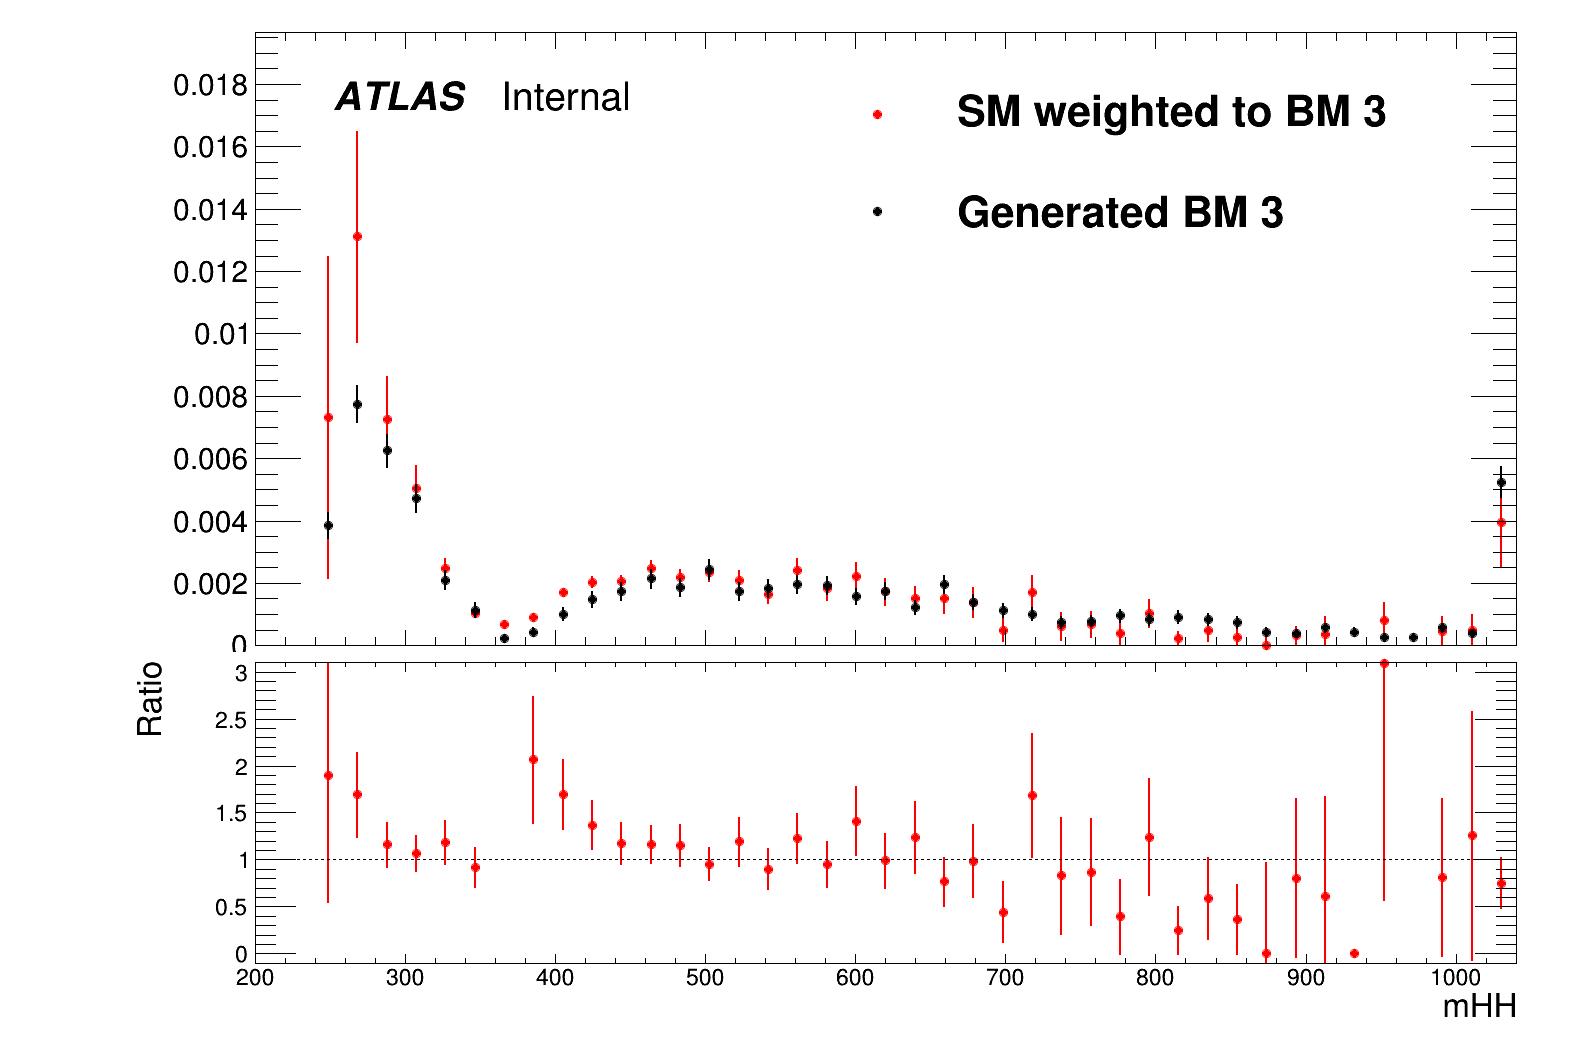
\includegraphics[width=.32\textwidth]{figures/Method_B_all_latest_LTT/BM3h_mHH.png}\\
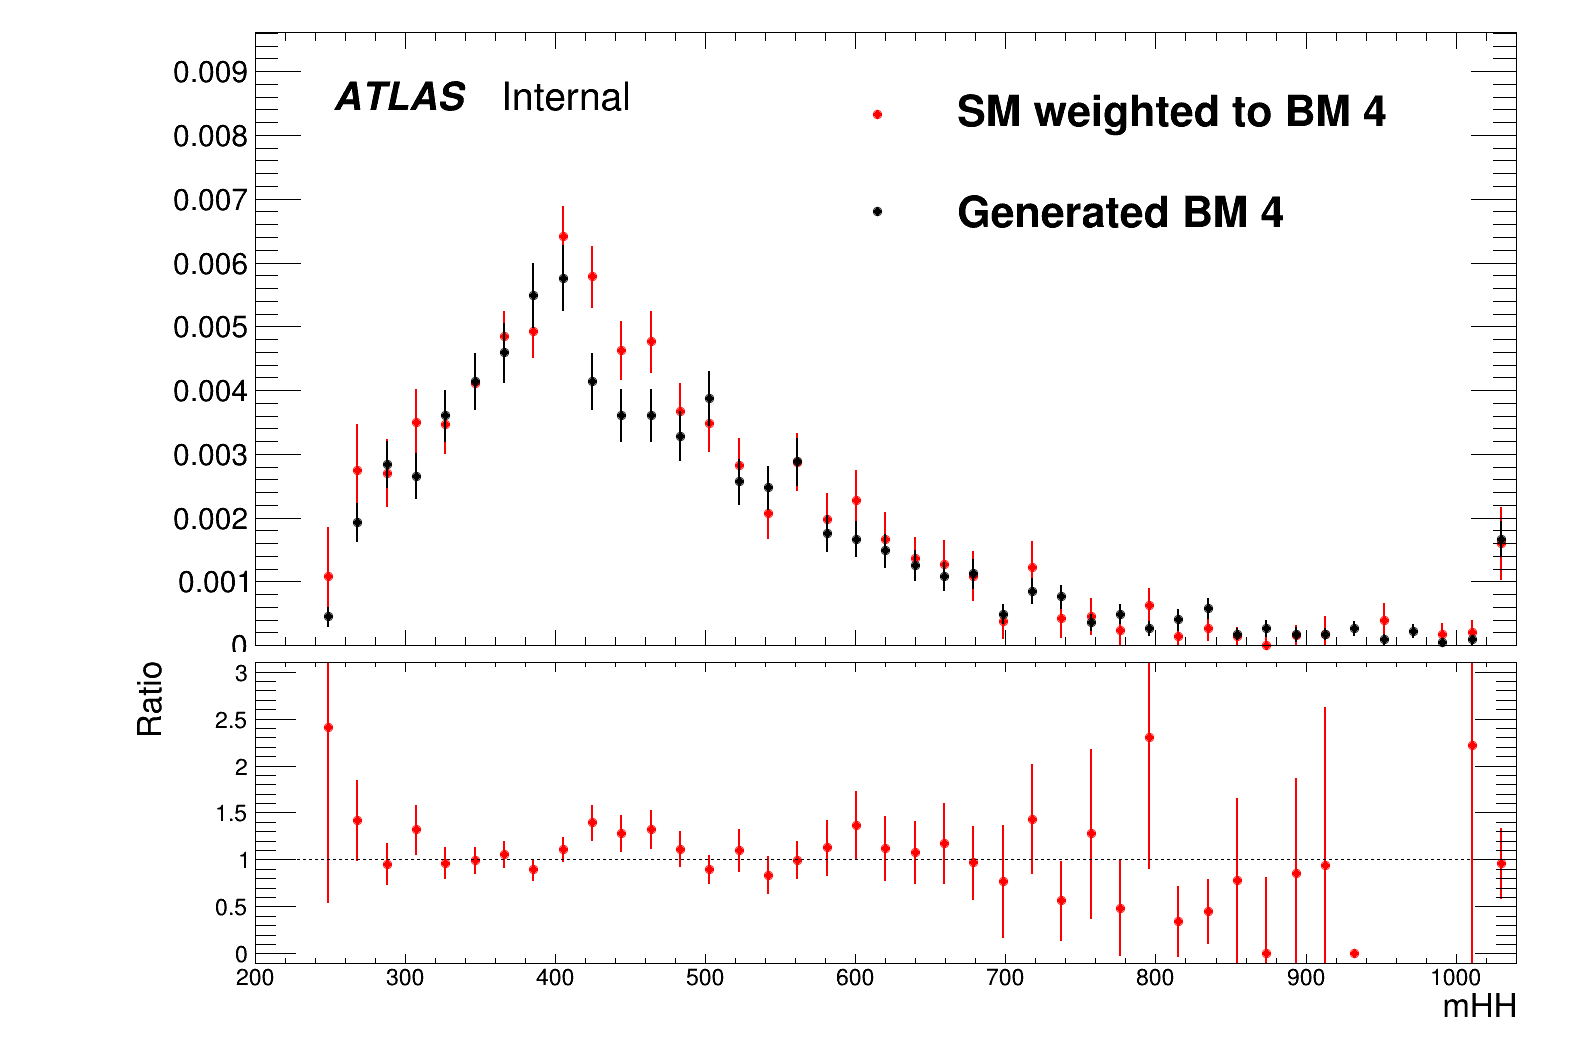
\includegraphics[width=.32\textwidth]{figures/Method_B_all_latest_LTT/BM4h_mHH.png}
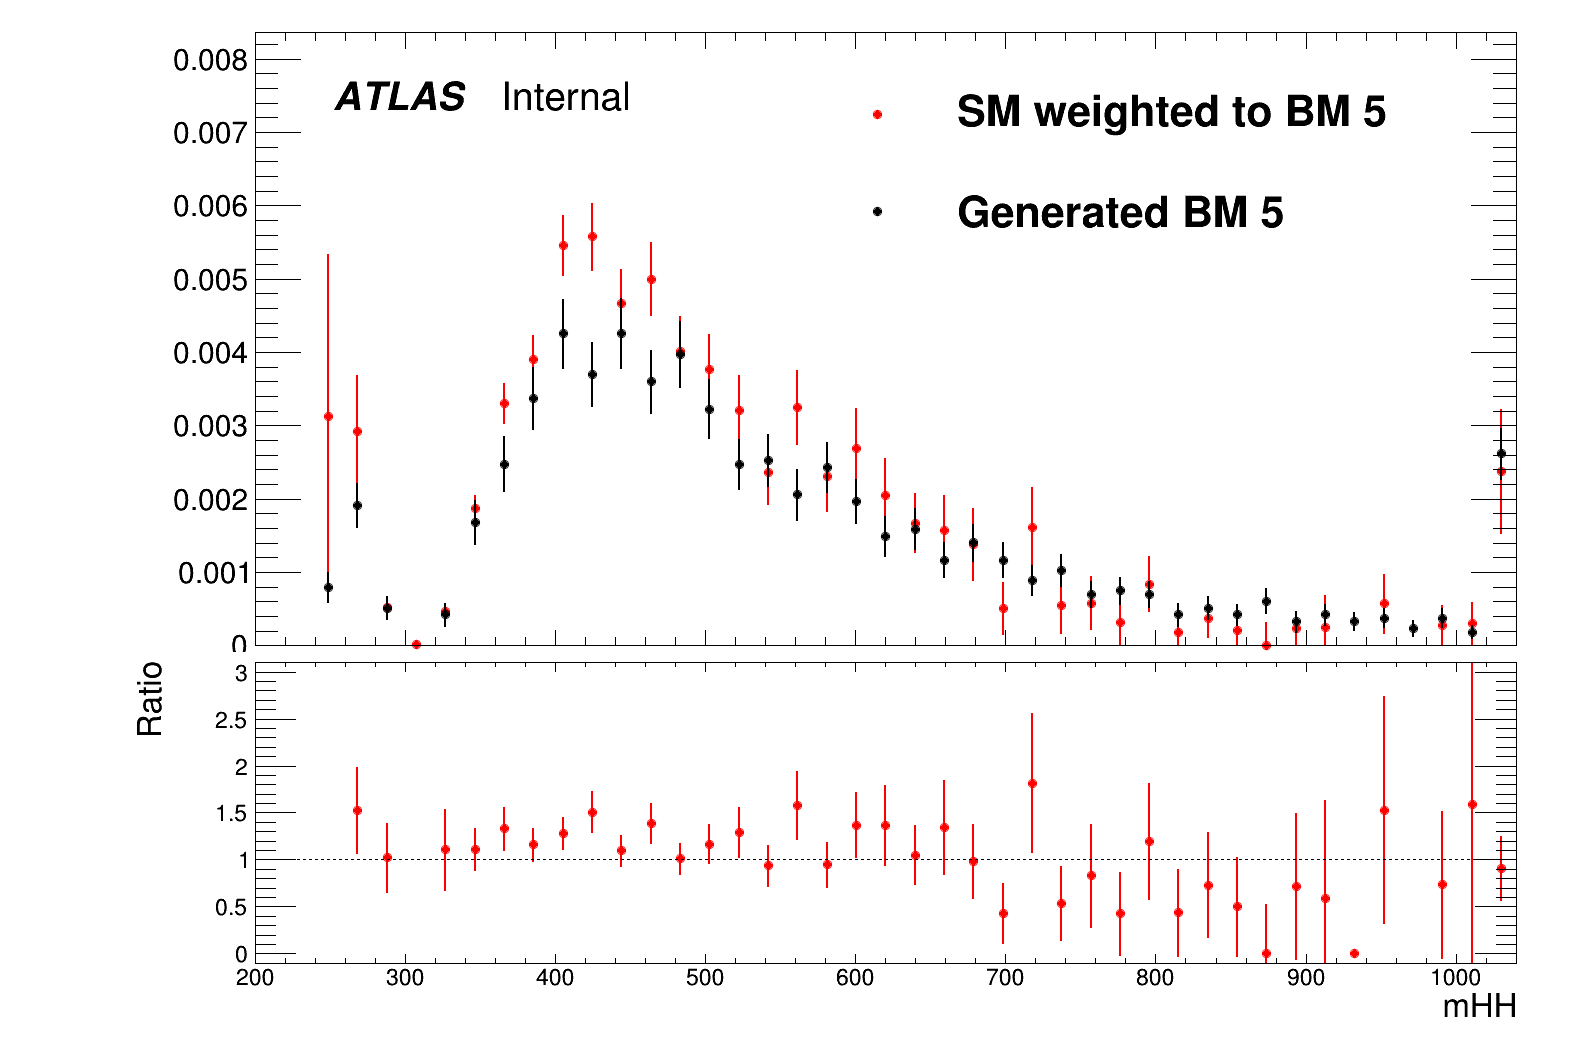
\includegraphics[width=.32\textwidth]{figures/Method_B_all_latest_LTT/BM5h_mHH.png}
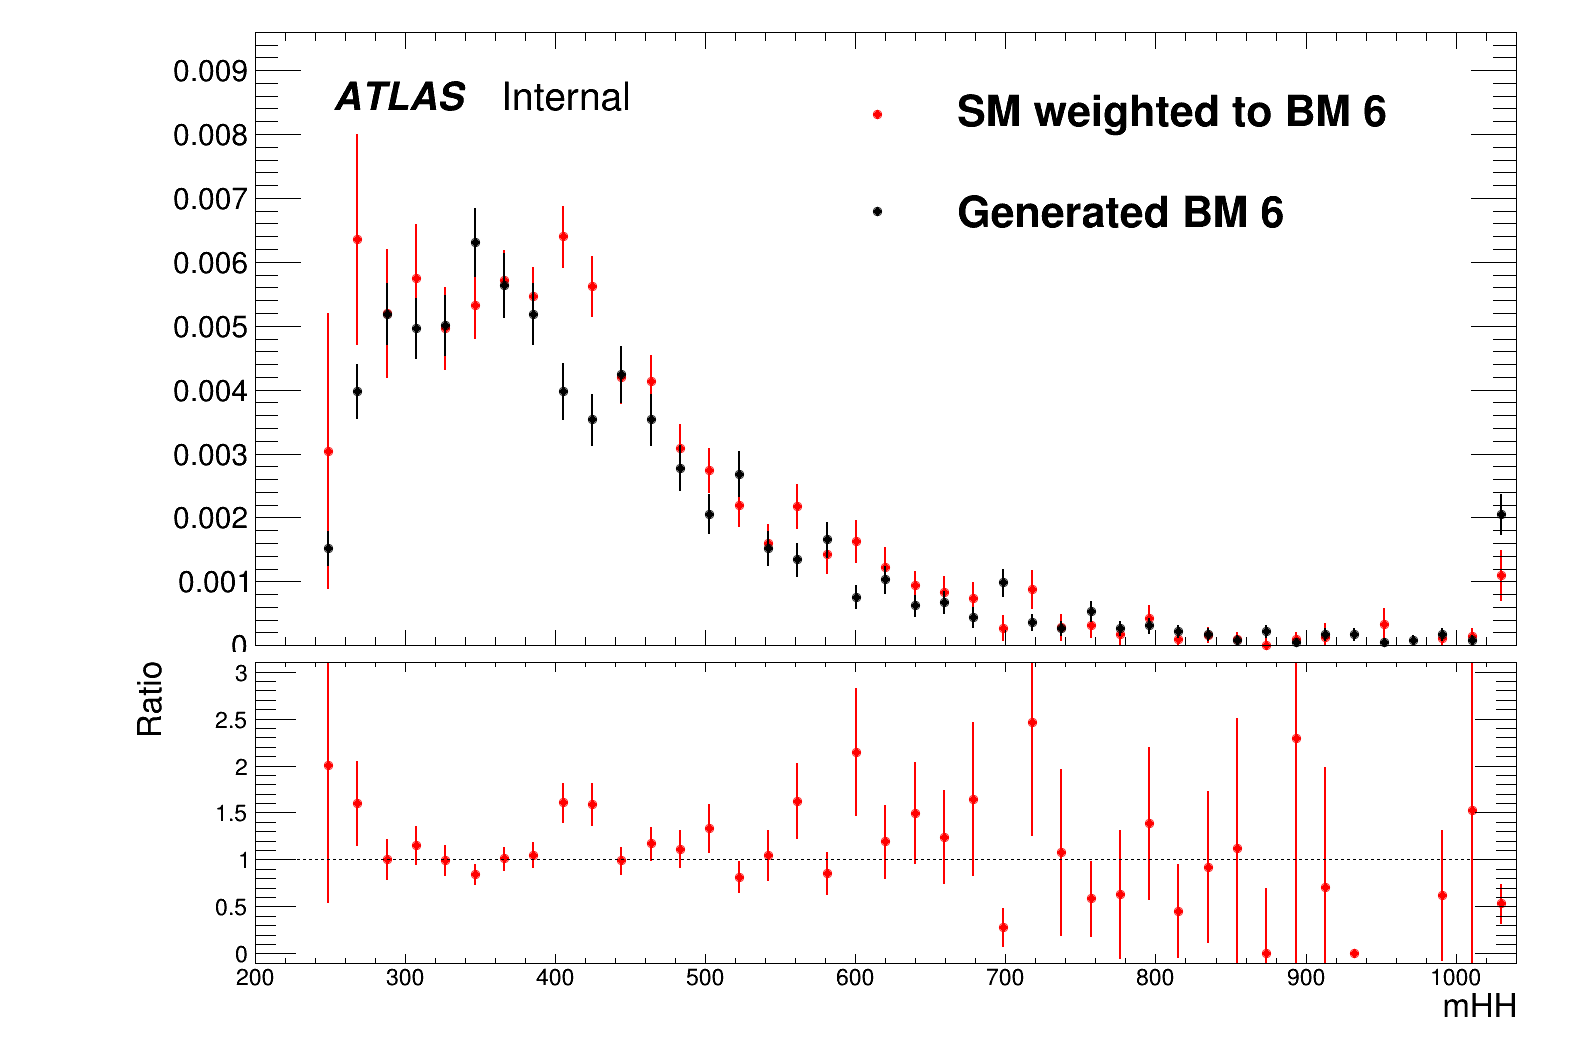
\includegraphics[width=.32\textwidth]{figures/Method_B_all_latest_LTT/BM6h_mHH.png}\\
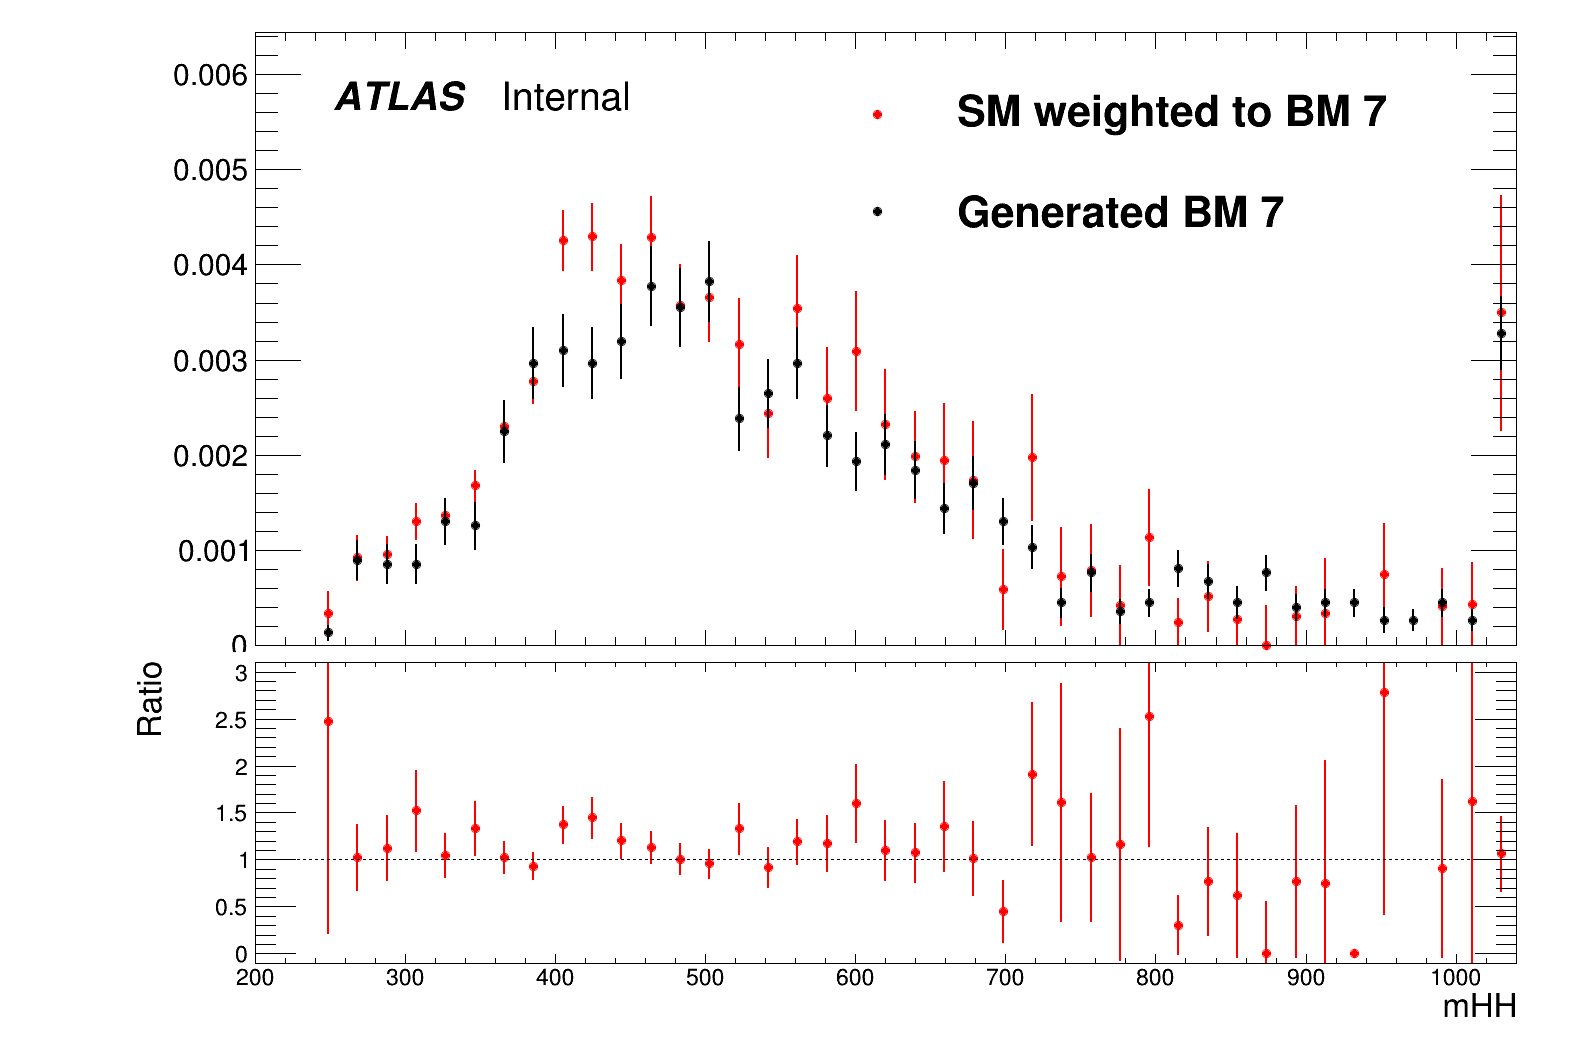
\includegraphics[width=.32\textwidth]{figures/Method_B_all_latest_LTT/BM7h_mHH.png}

\end{frame}


\begin{frame}
\frametitle{LTT $c_{ggHH}$ scan $\Delta R_{\tau\tau}$ shape: weighted SM vs generated BM}

\begin{figure}
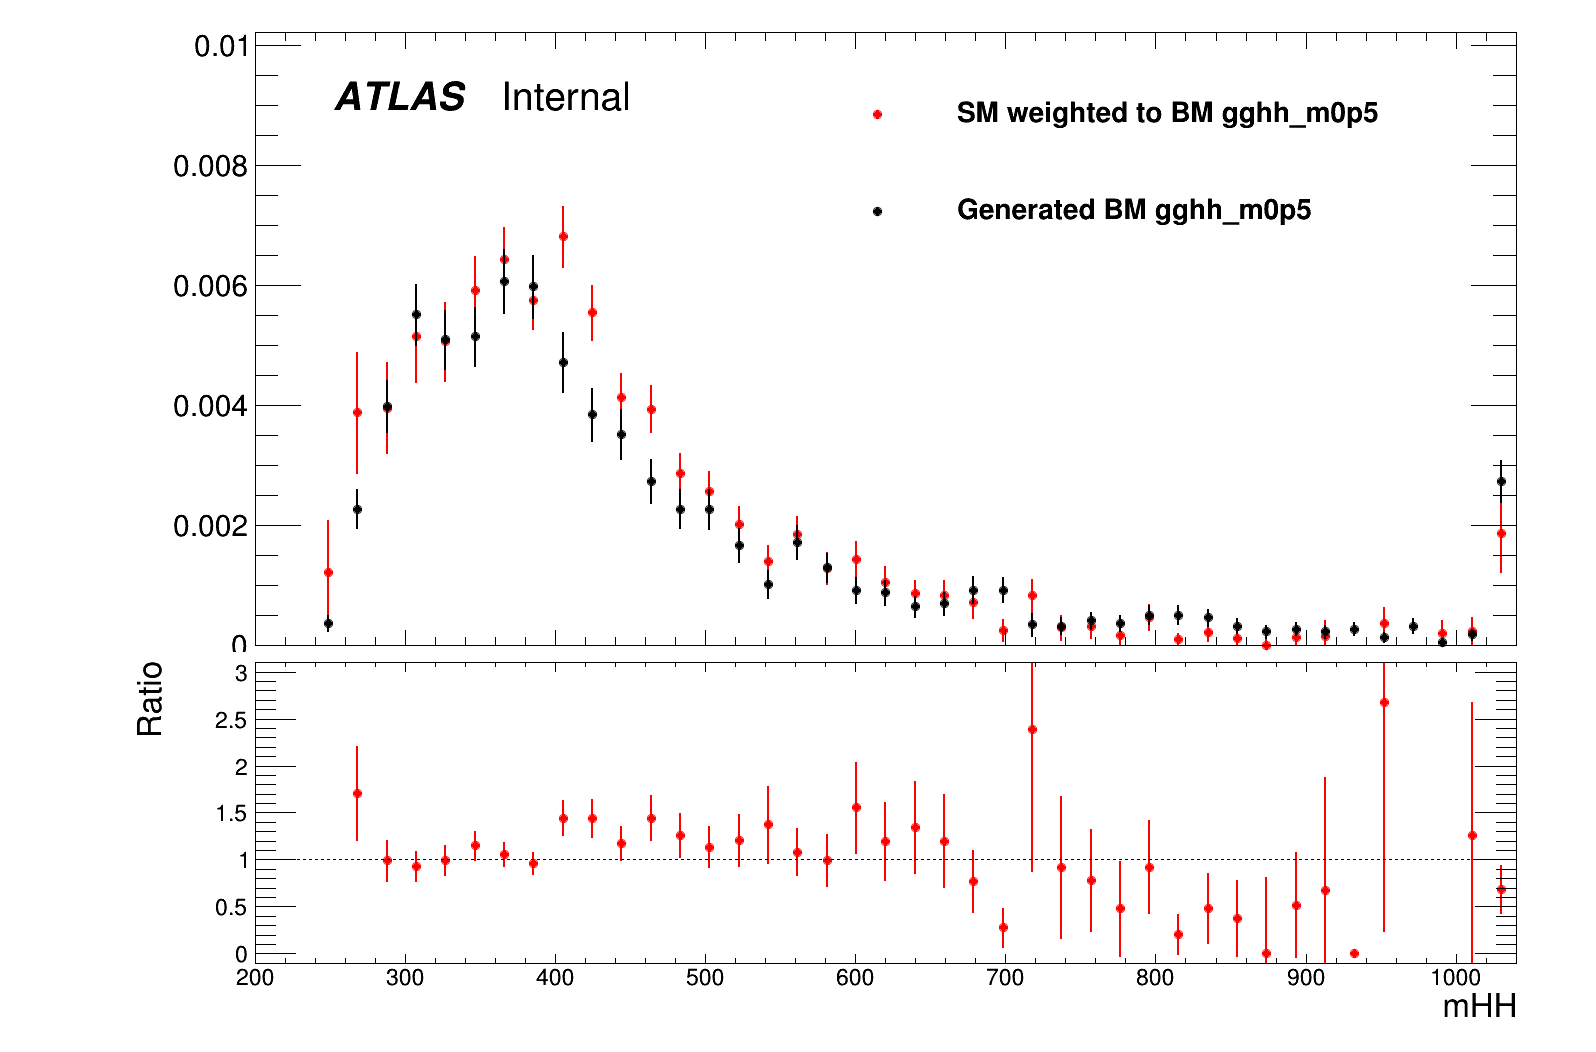
\includegraphics[width=.32\textwidth]{figures/Method_B_all_latest_LTT/BMgghh_m0p5h_mHH.png}
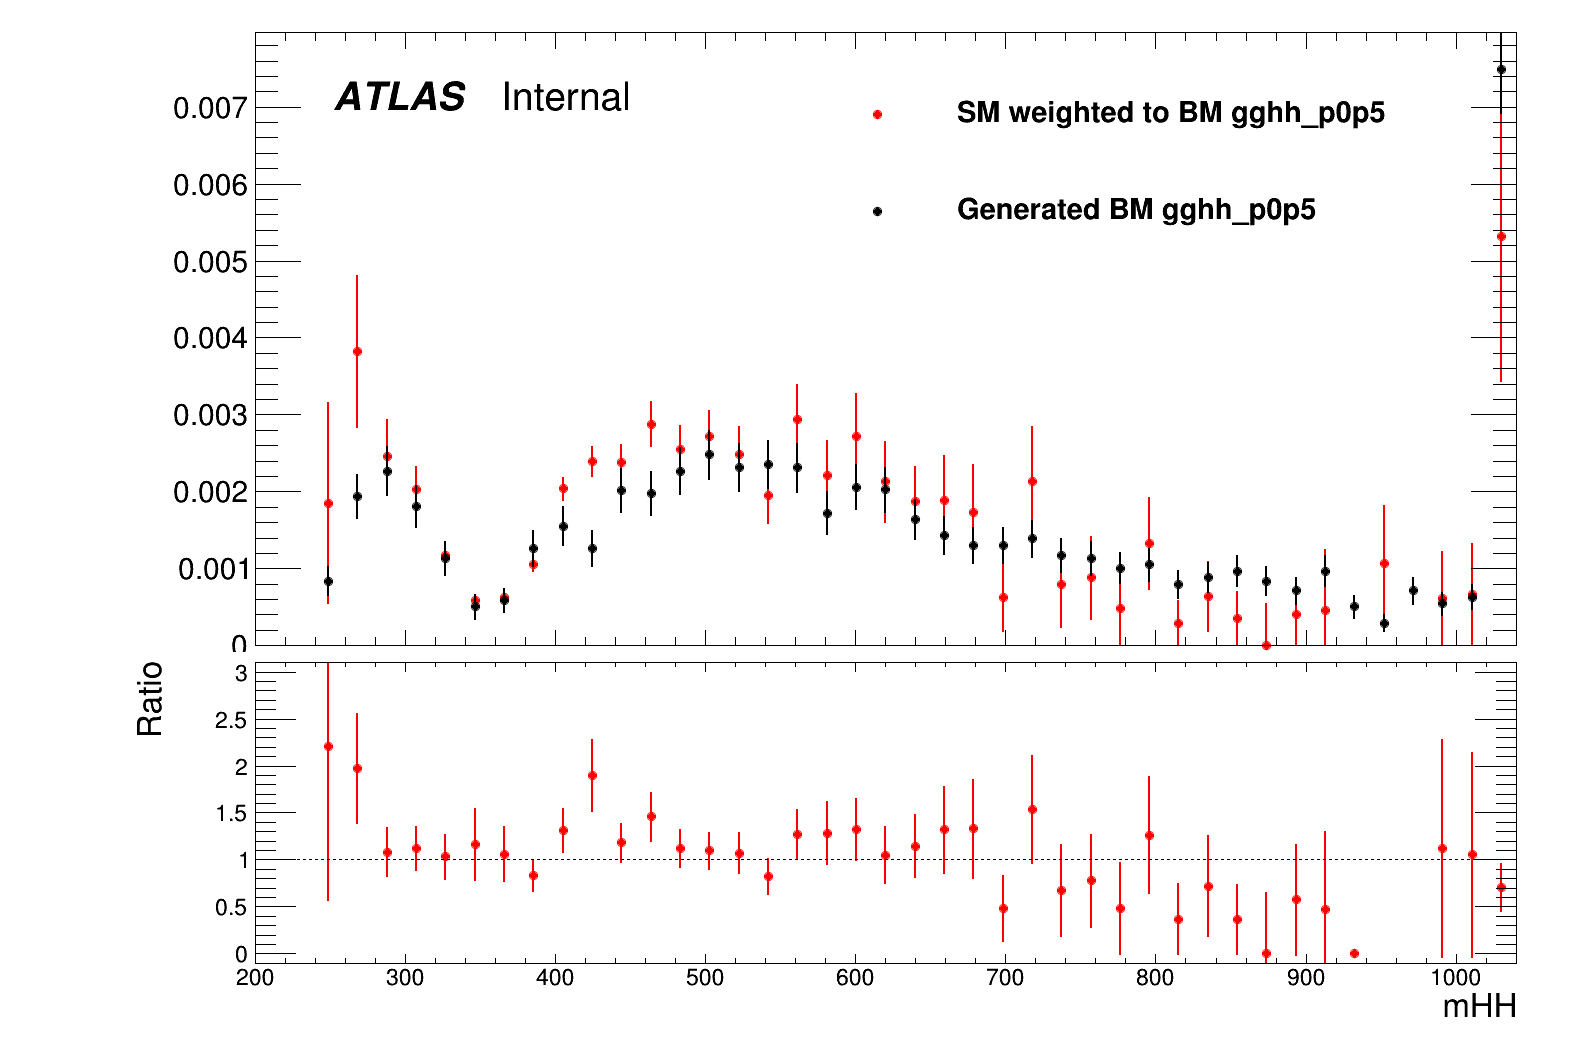
\includegraphics[width=.32\textwidth]{figures/Method_B_all_latest_LTT/BMgghh_p0p5h_mHH.png}
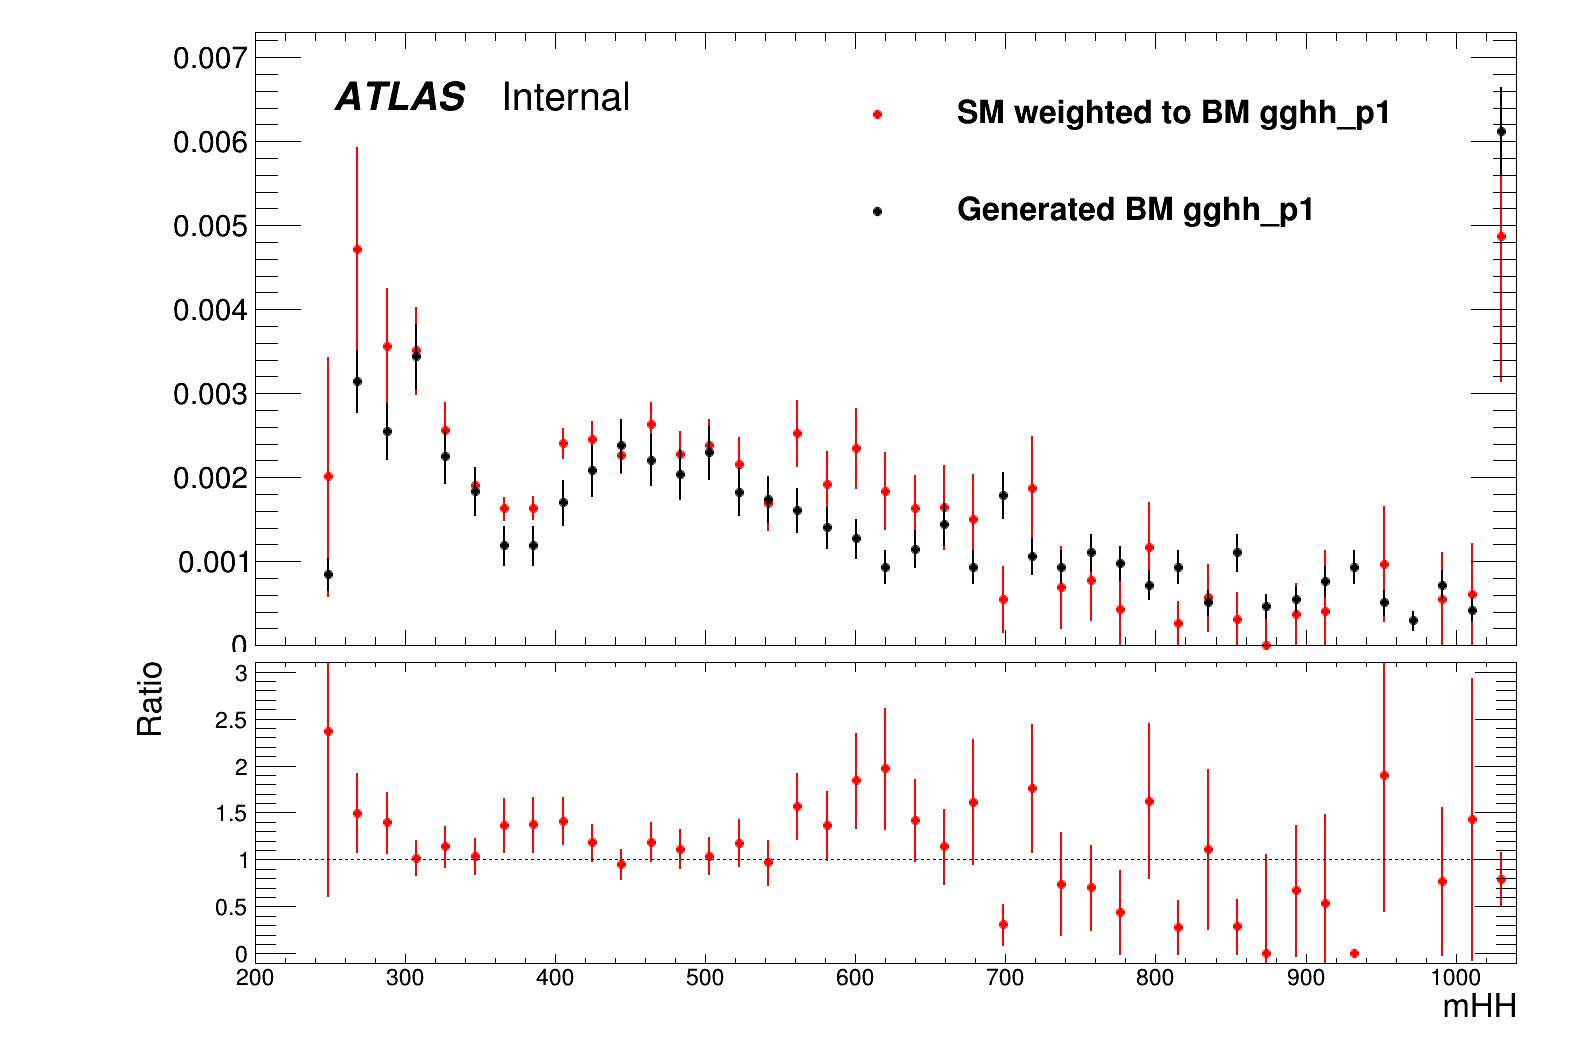
\includegraphics[width=.32\textwidth]{figures/Method_B_all_latest_LTT/BMgghh_p1h_mHH.png}
$c_{ggHH} = -0.5$ \hspace{5em} $c_{ggHH} = 0.5$\hspace{5em} $c_{ggHH} = 1.0$
\end{figure}


\end{frame}     

\begin{frame}
\frametitle{LTT $c_{ttHH}$ scan $\Delta R_{\tau\tau}$ shape: weighted SM vs generated BM}
\begin{figure}
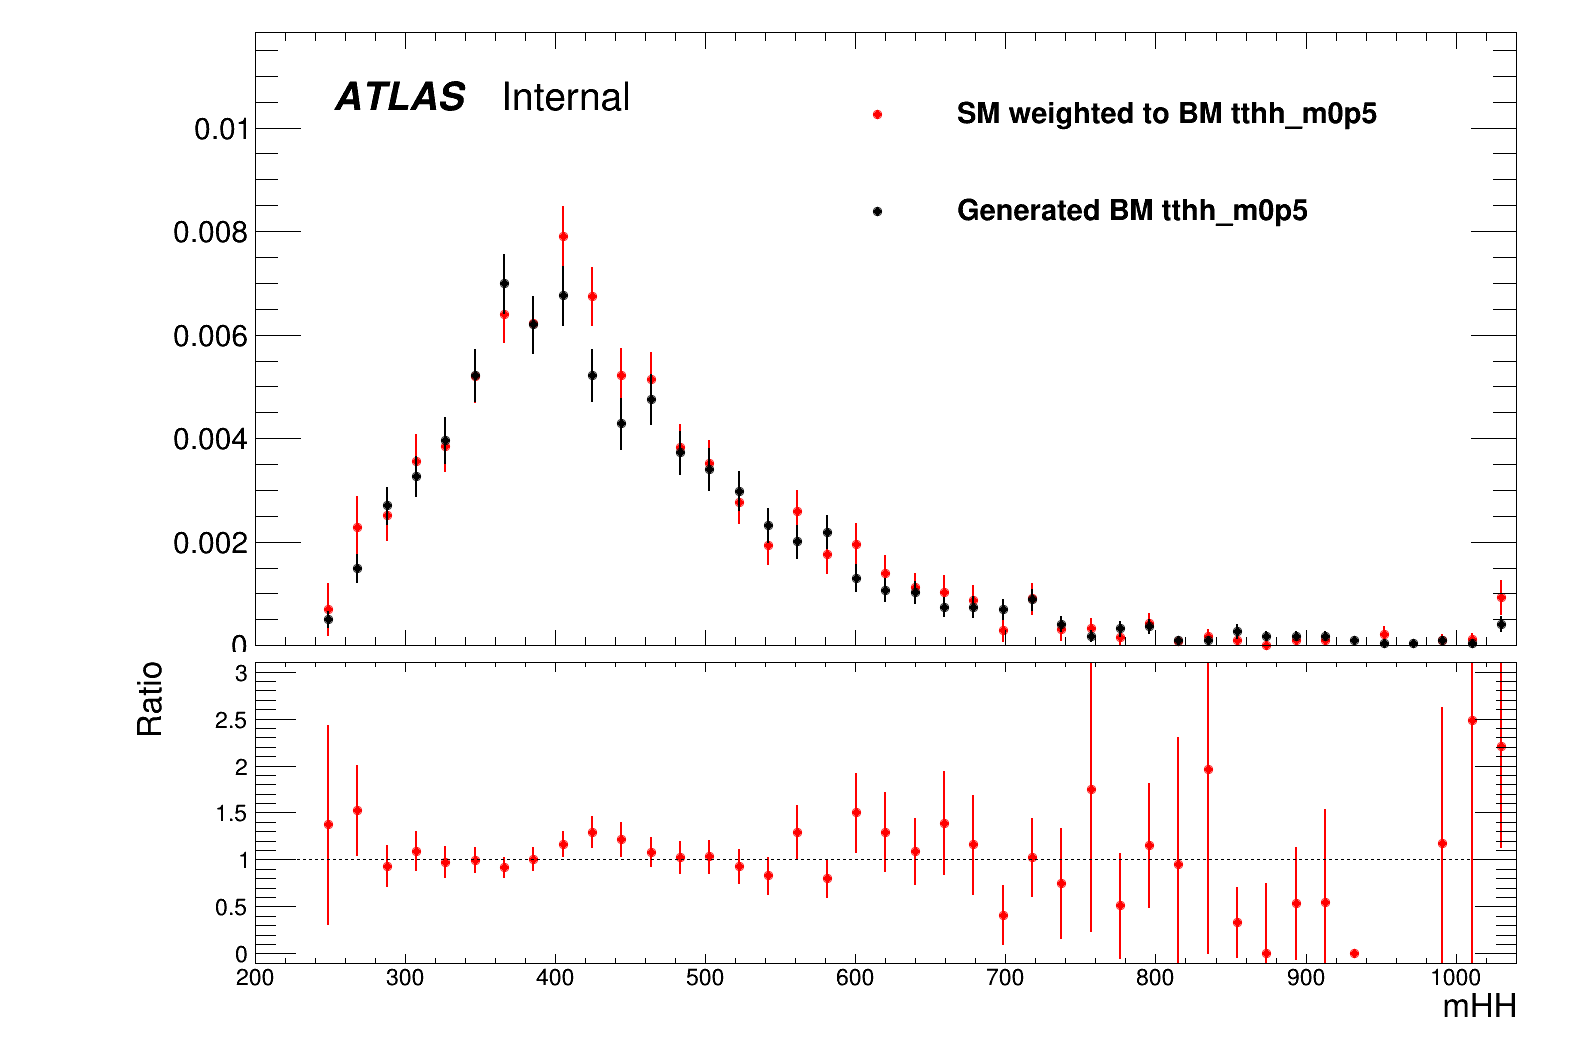
\includegraphics[width=.32\textwidth]{figures/Method_B_all_latest_LTT/BMtthh_m0p5h_mHH.png}
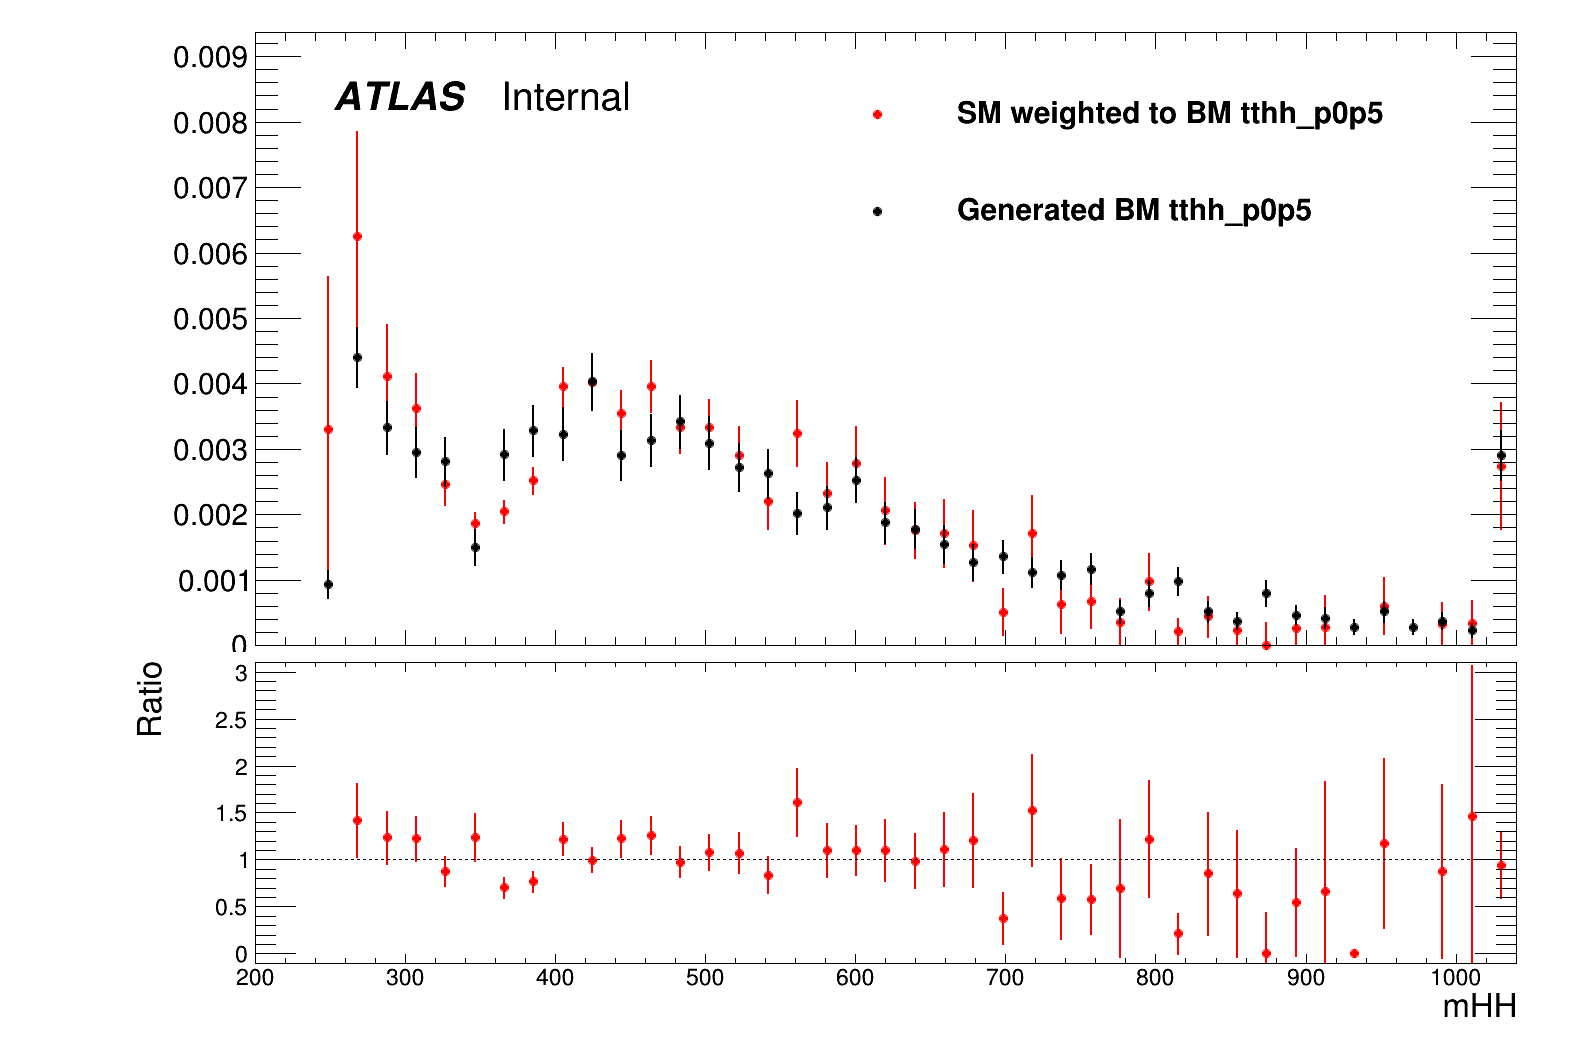
\includegraphics[width=.32\textwidth]{figures/Method_B_all_latest_LTT/BMtthh_p0p5h_mHH.png}
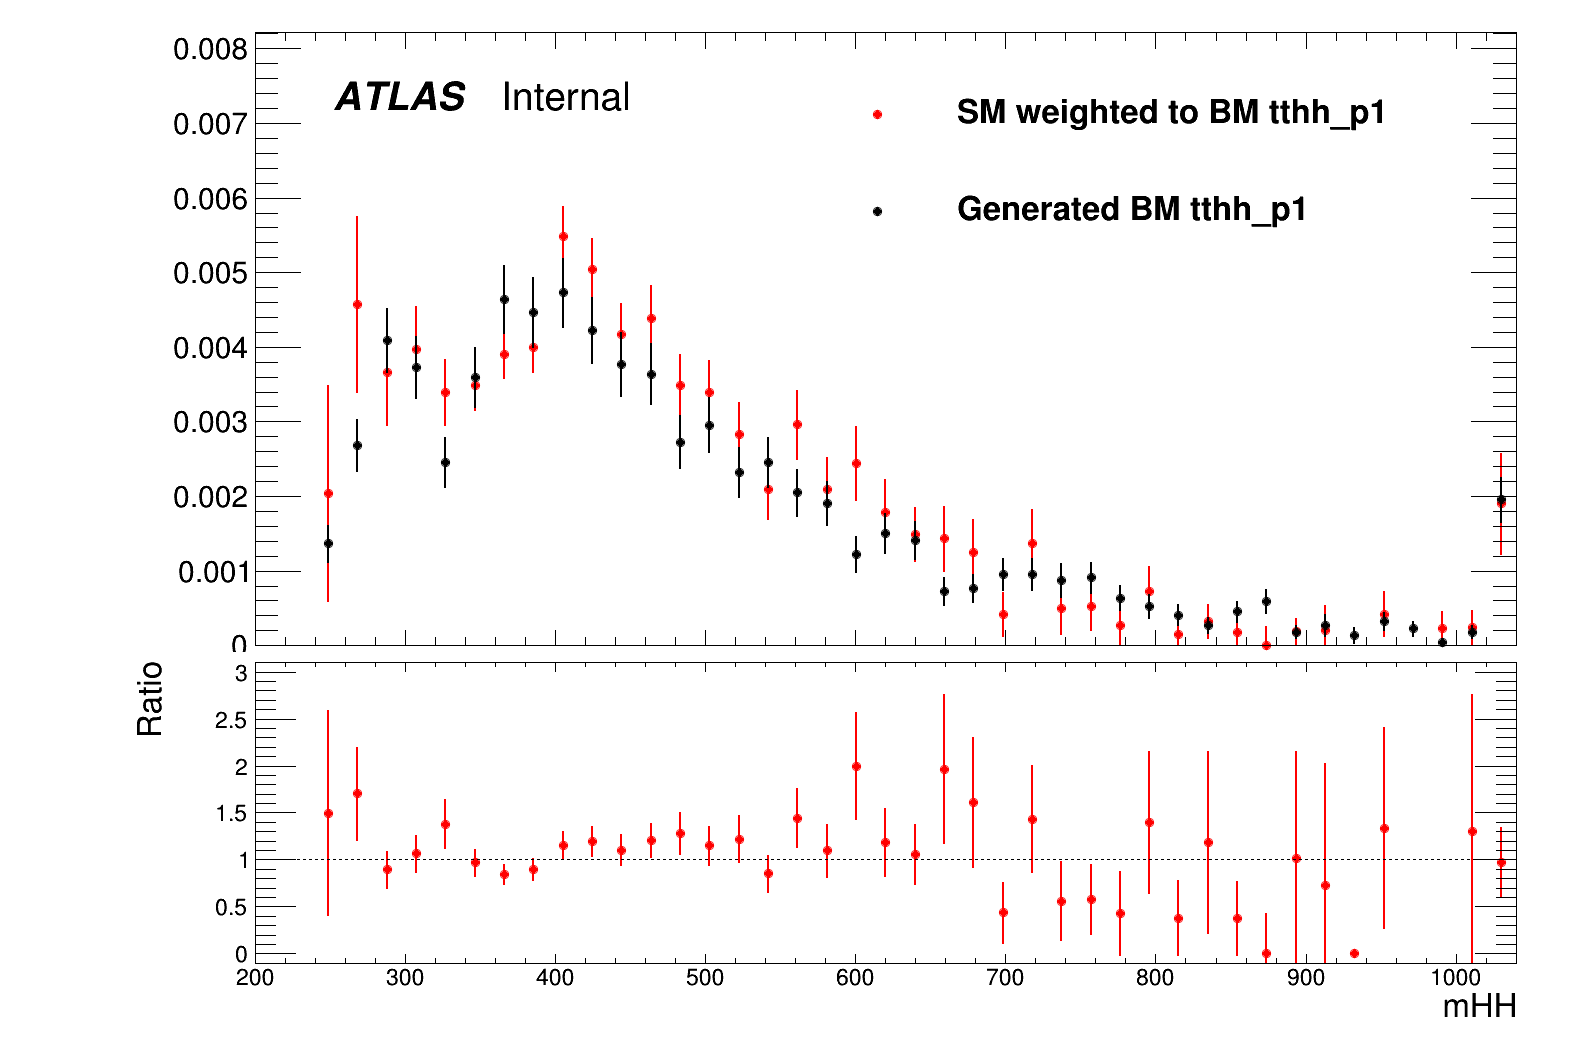
\includegraphics[width=.32\textwidth]{figures/Method_B_all_latest_LTT/BMtthh_p1h_mHH.png}
$c_{ttHH} = -0.5$ \hspace{5em} $c_{ttHH} = 0.5$\hspace{5em} $c_{ttHH} = 1.0$    
\end{figure}

\end{frame}   


\begin{frame}   

\begin{table}
    \begin{tabular}{l | l | l|}
    BM points (parameter values)   & SLT & LTT \\
        \hline
        \hline
       gghh:-0.5& 0.92 $\pm$ 0.03 & 1.11 $\pm$ 0.04 \\
       gghh:1.0& 0.9 $\pm$ 0.04 & 1.09 $\pm$ 0.06 \\
       gghh:0.5& 0.9 $\pm$ 0.04 & 1.04 $\pm$ 0.06 \\
       tthh:0.5& 0.96 $\pm$ 0.03 & 1.06 $\pm$ 0.06 \\
       tthh:-0.5& 0.96 $\pm$ 0.02 & 1.07 $\pm$ 0.04 \\
       tthh:1.0& 0.98 $\pm$ 0.03 & 1.1 $\pm$ 0.05 \\
        BM1& 0.85 $\pm$ 0.06 & 1.08 $\pm$ 0.13 \\
        BM2& 0.87 $\pm$ 0.04 & 1.06 $\pm$ 0.09 \\
        BM3& 0.9 $\pm$ 0.04 & 1.14 $\pm$ 0.09 \\
        BM4& 0.98 $\pm$ 0.03 & 1.08 $\pm$ 0.04 \\
        BM5& 0.92 $\pm$ 0.03 & 1.17 $\pm$ 0.05 \\
        BM6& 0.97 $\pm$ 0.03 & 1.14 $\pm$ 0.05 \\
        BM7& 0.99 $\pm$ 0.03 & 1.12 $\pm$ 0.05 \\
    \end{tabular}
    \caption{yield ratios: weighted SM divided by generated BMs}
    \end{table}

\end{frame}   


\begin{frame}
    \frametitle{Conclusion}
    \begin{itemize}
    \item No significant shape dependence
    \item assigning the difference from 1 of the yields ratios as the uncertainty
    \end{itemize}
\end{frame} 


\begin{frame}
    \frametitle{Bkp: SLT BMs $\Delta R_{\tau\tau}$ shape: weighted SM vs generated BM}
\centering  
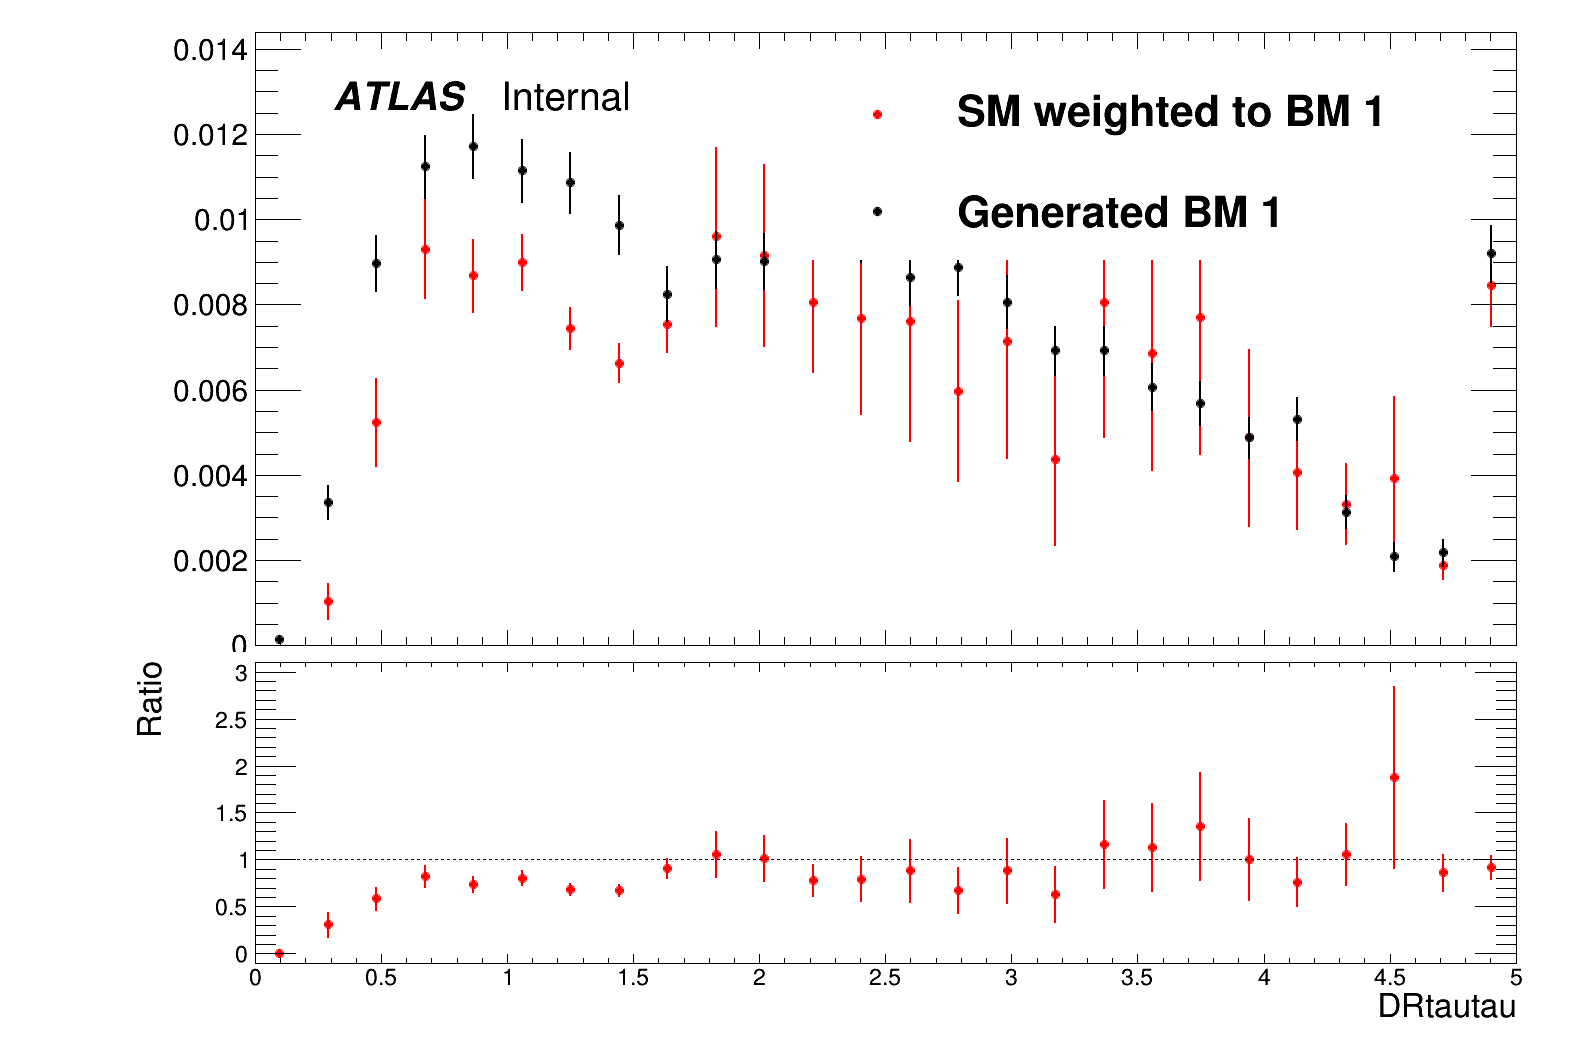
\includegraphics[width=.32\textwidth]{figures/Method_B_all_latest/BM1h_DRtautau.png}
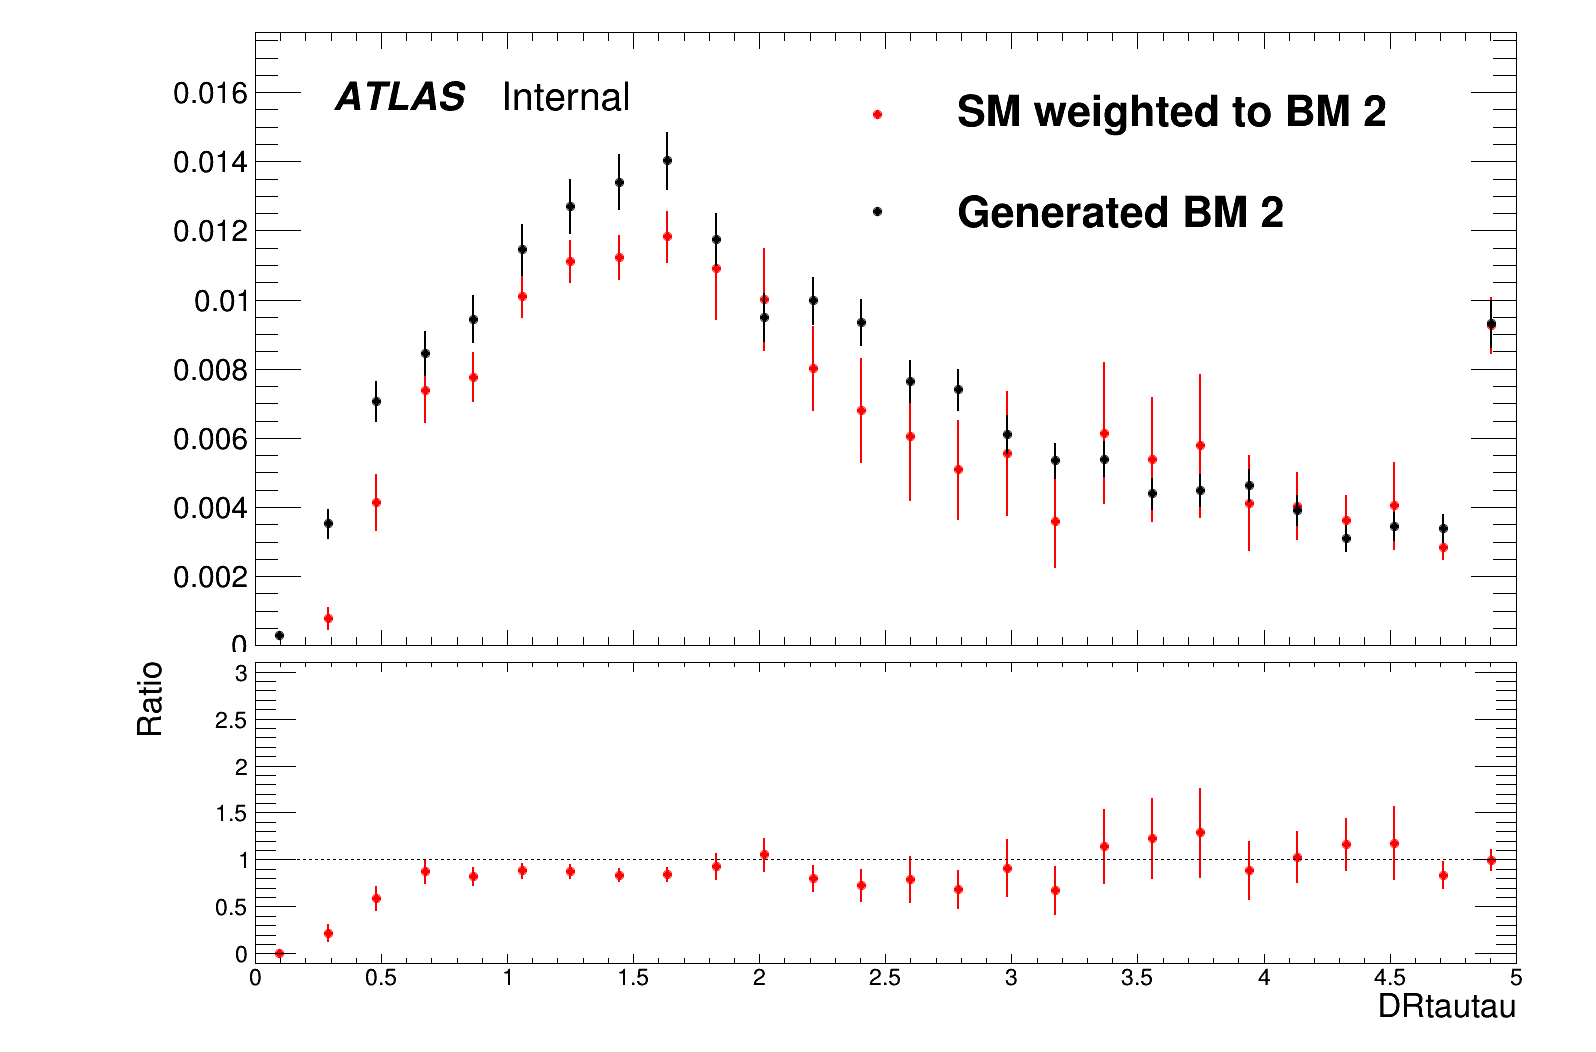
\includegraphics[width=.32\textwidth]{figures/Method_B_all_latest/BM2h_DRtautau.png}
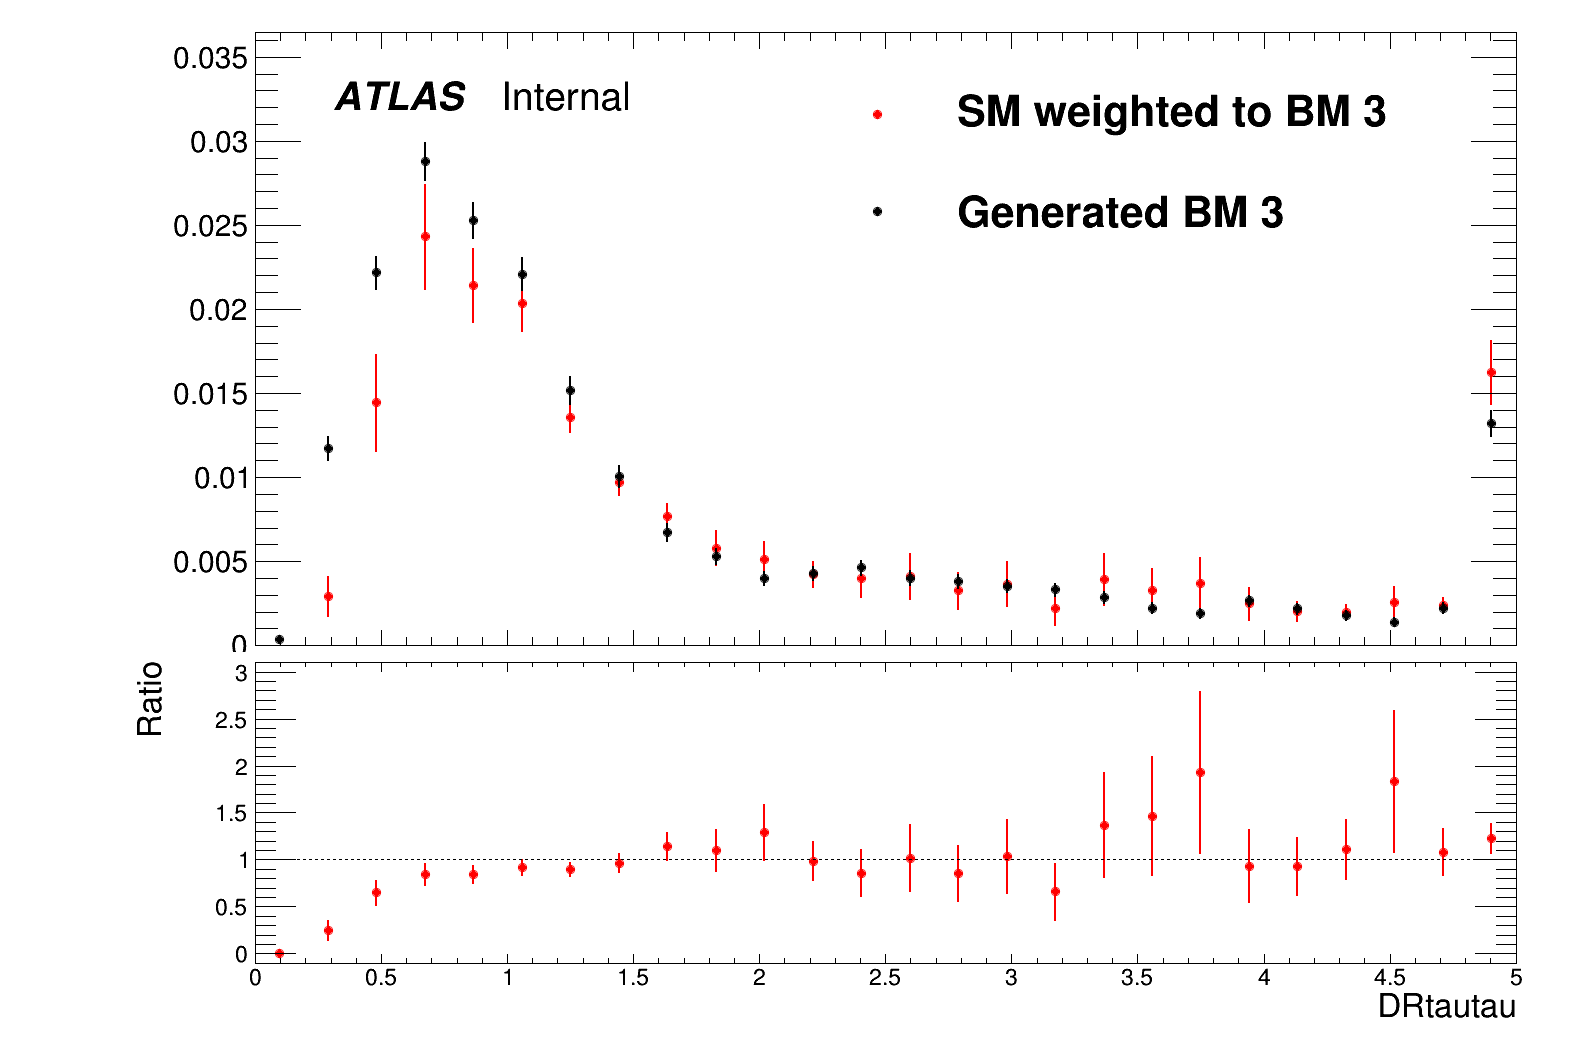
\includegraphics[width=.32\textwidth]{figures/Method_B_all_latest/BM3h_DRtautau.png}\\
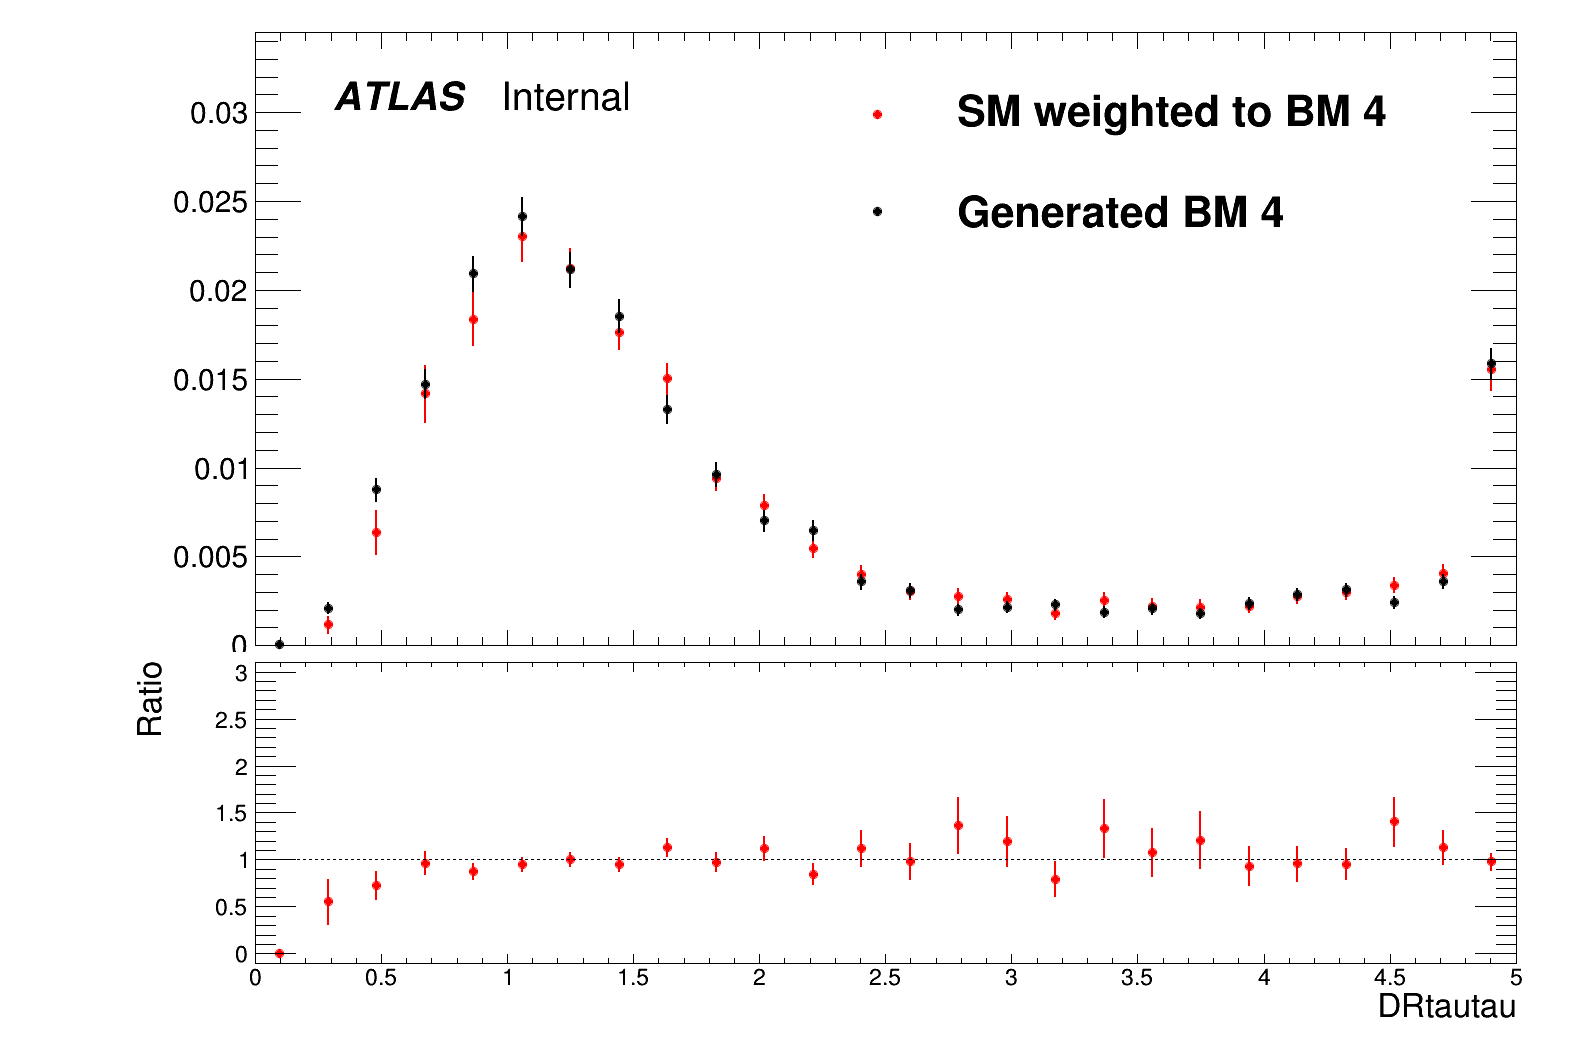
\includegraphics[width=.32\textwidth]{figures/Method_B_all_latest/BM4h_DRtautau.png}
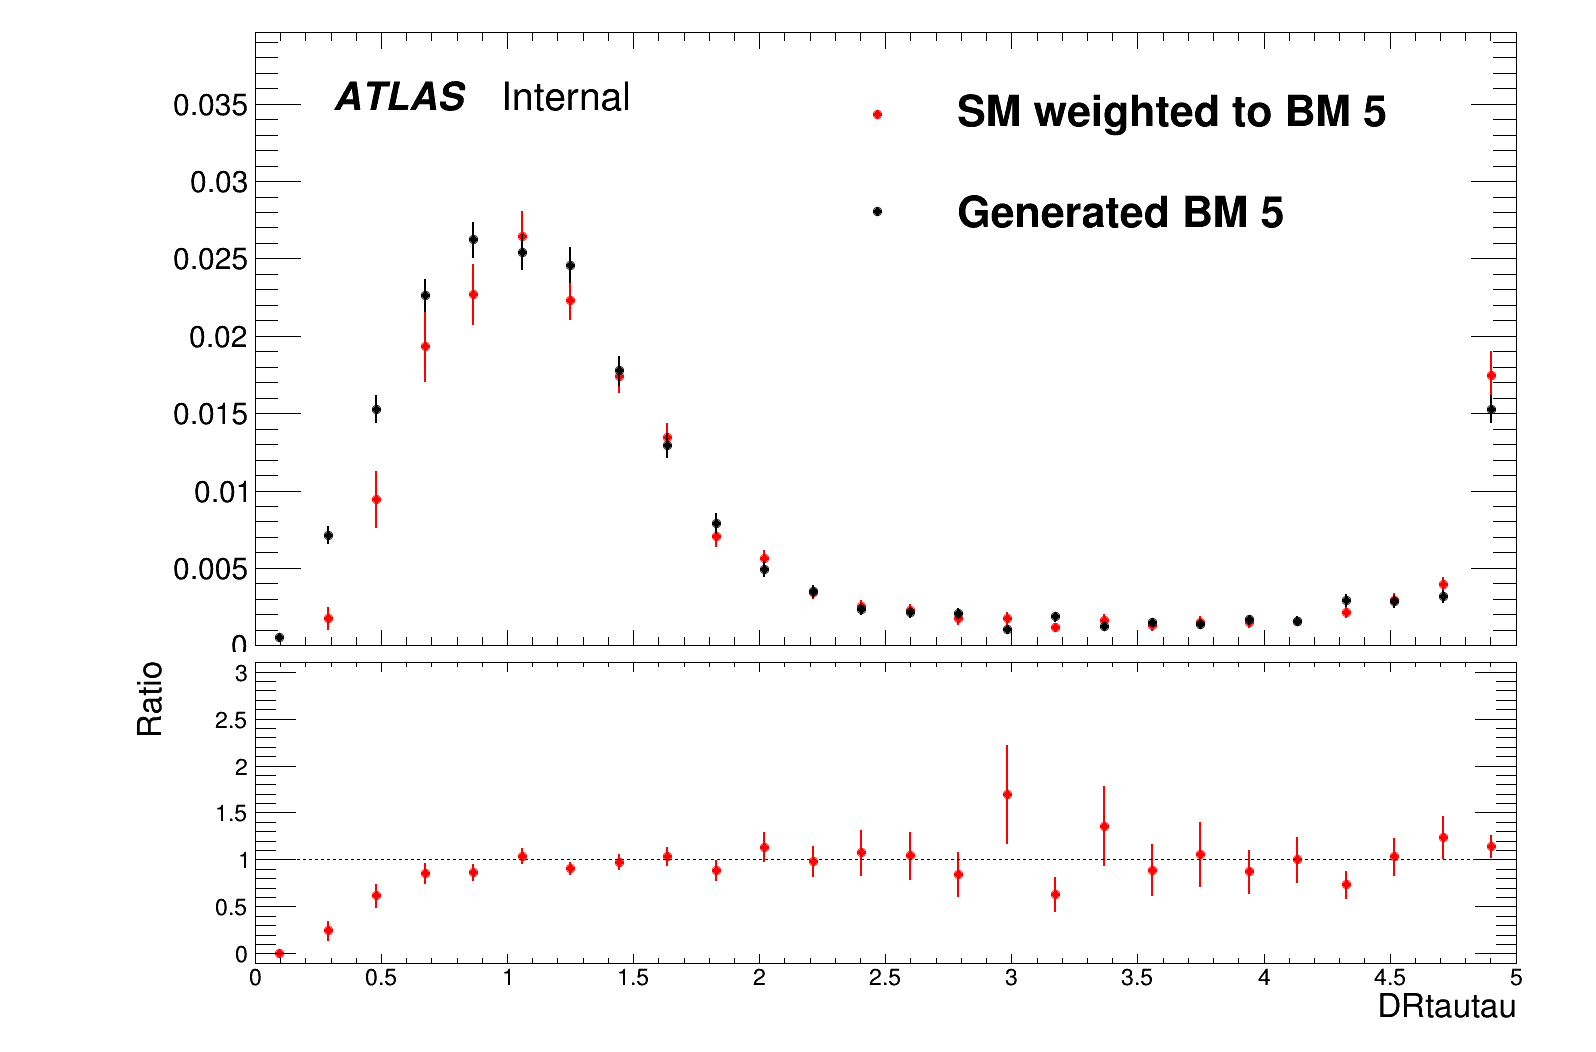
\includegraphics[width=.32\textwidth]{figures/Method_B_all_latest/BM5h_DRtautau.png}
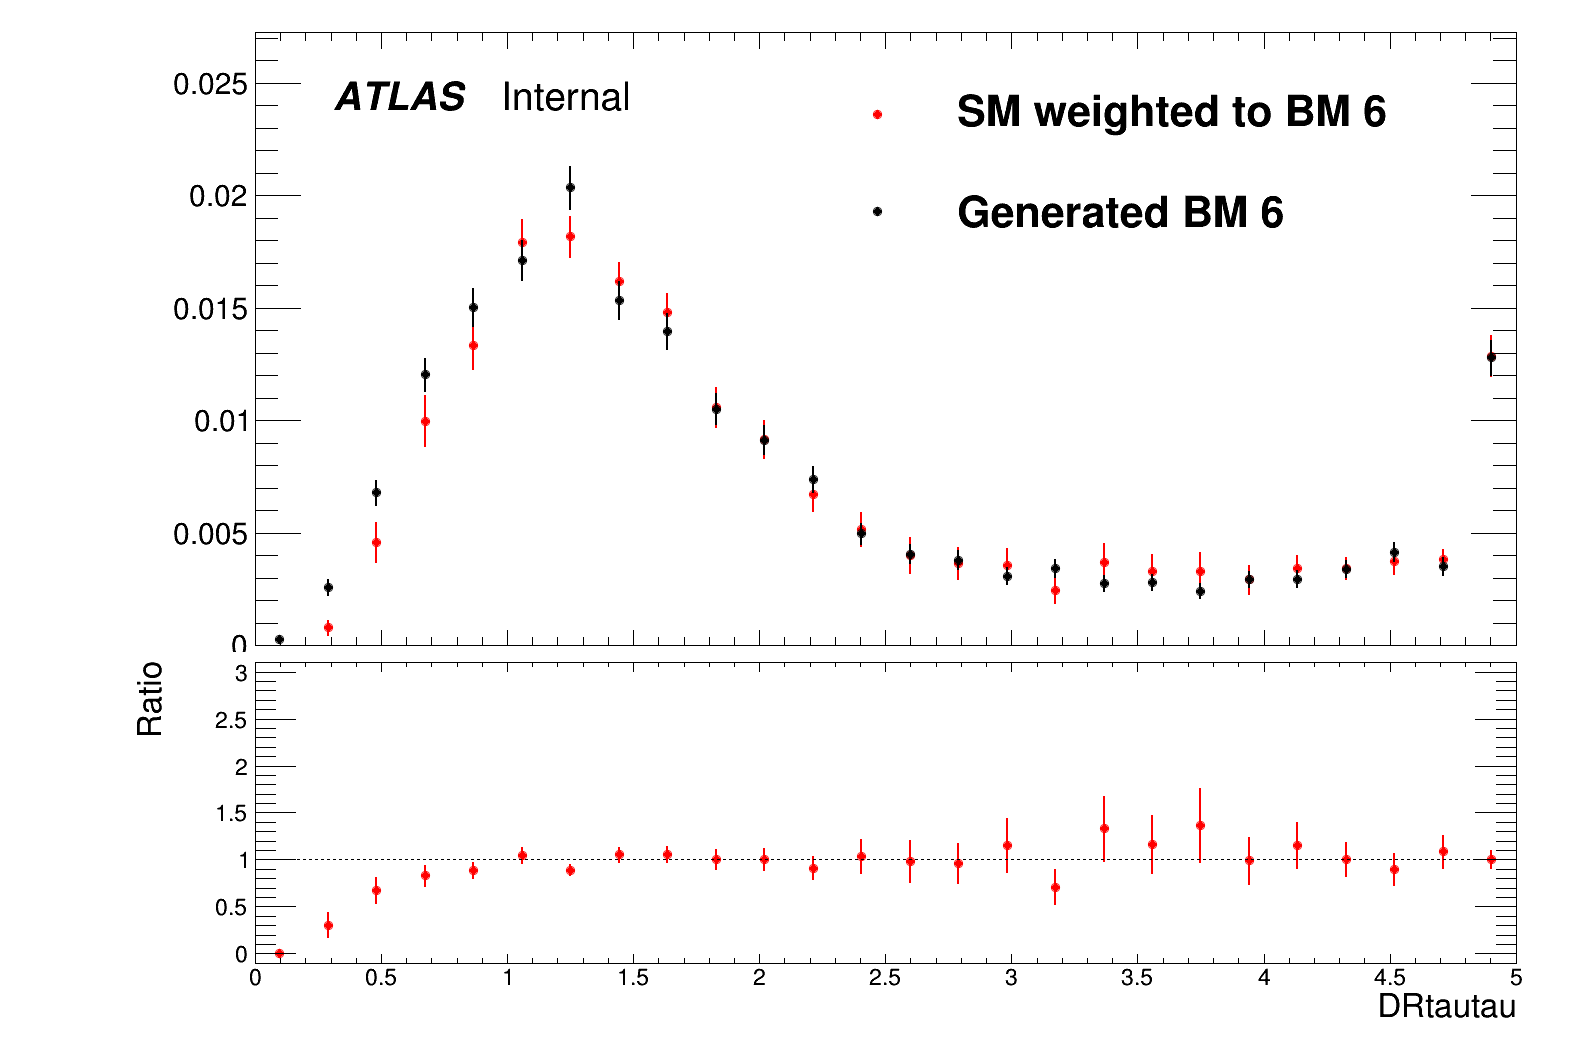
\includegraphics[width=.32\textwidth]{figures/Method_B_all_latest/BM6h_DRtautau.png}\\
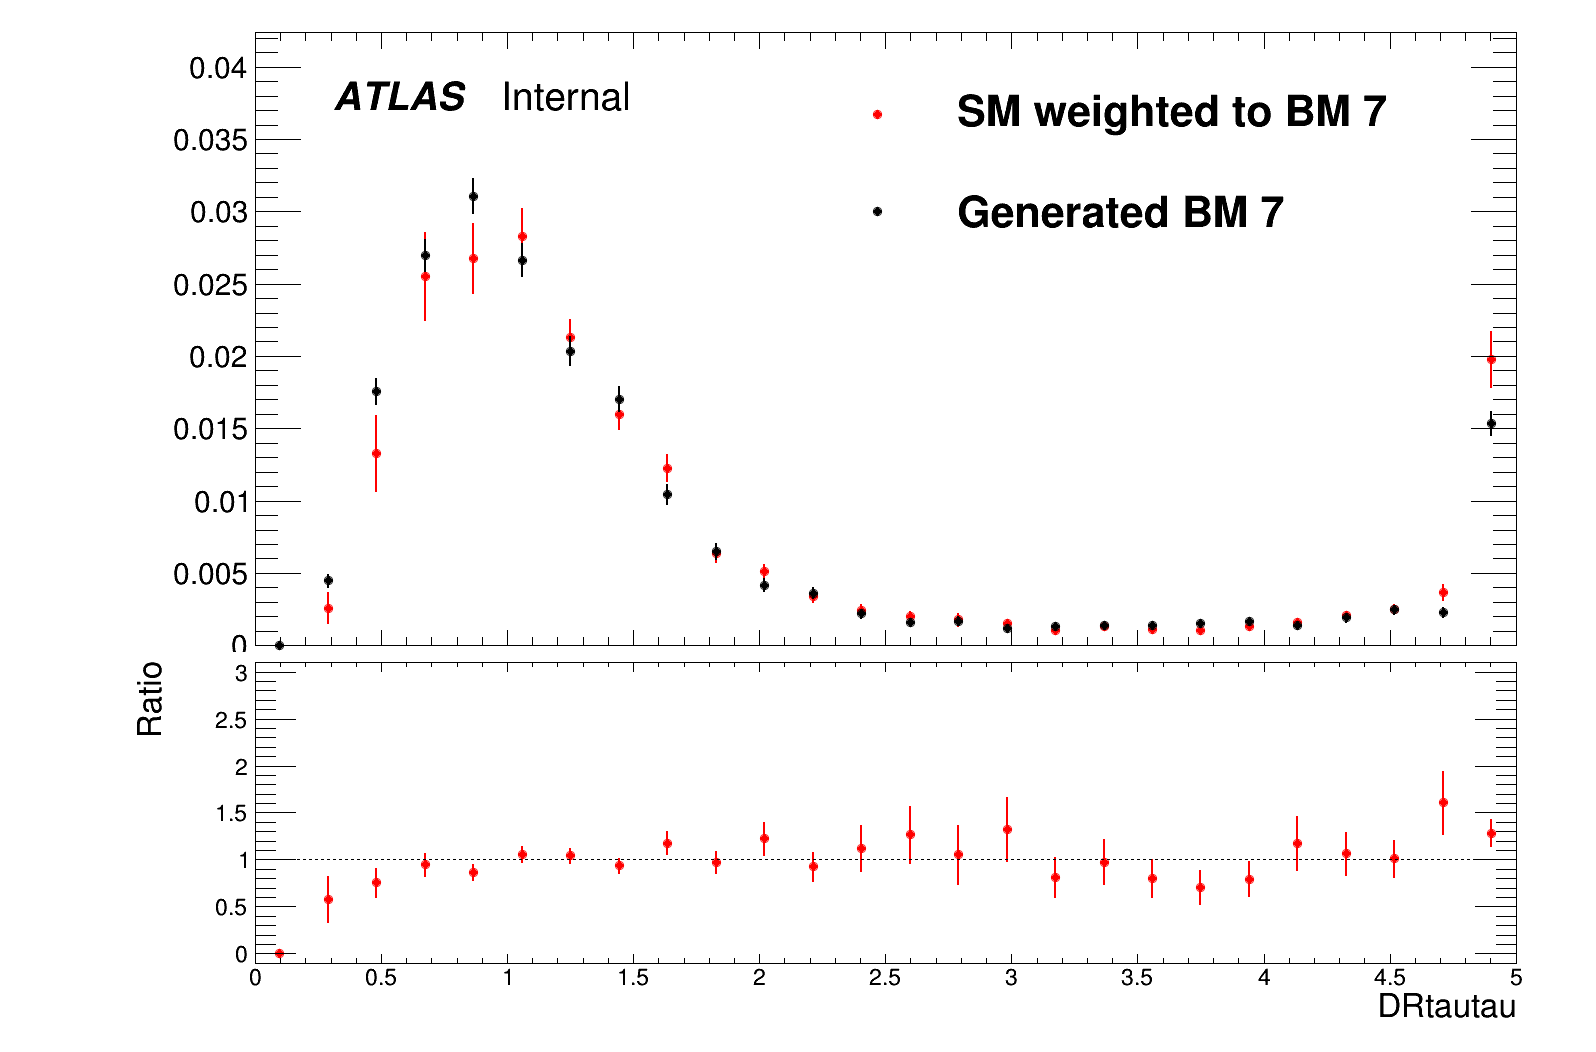
\includegraphics[width=.32\textwidth]{figures/Method_B_all_latest/BM7h_DRtautau.png}

\end{frame}

\begin{frame}
    \frametitle{Bkp: SLT $c_{ggHH}$ scan $\Delta R_{\tau\tau}$ shape: weighted SM vs generated BM}

    \begin{figure}
    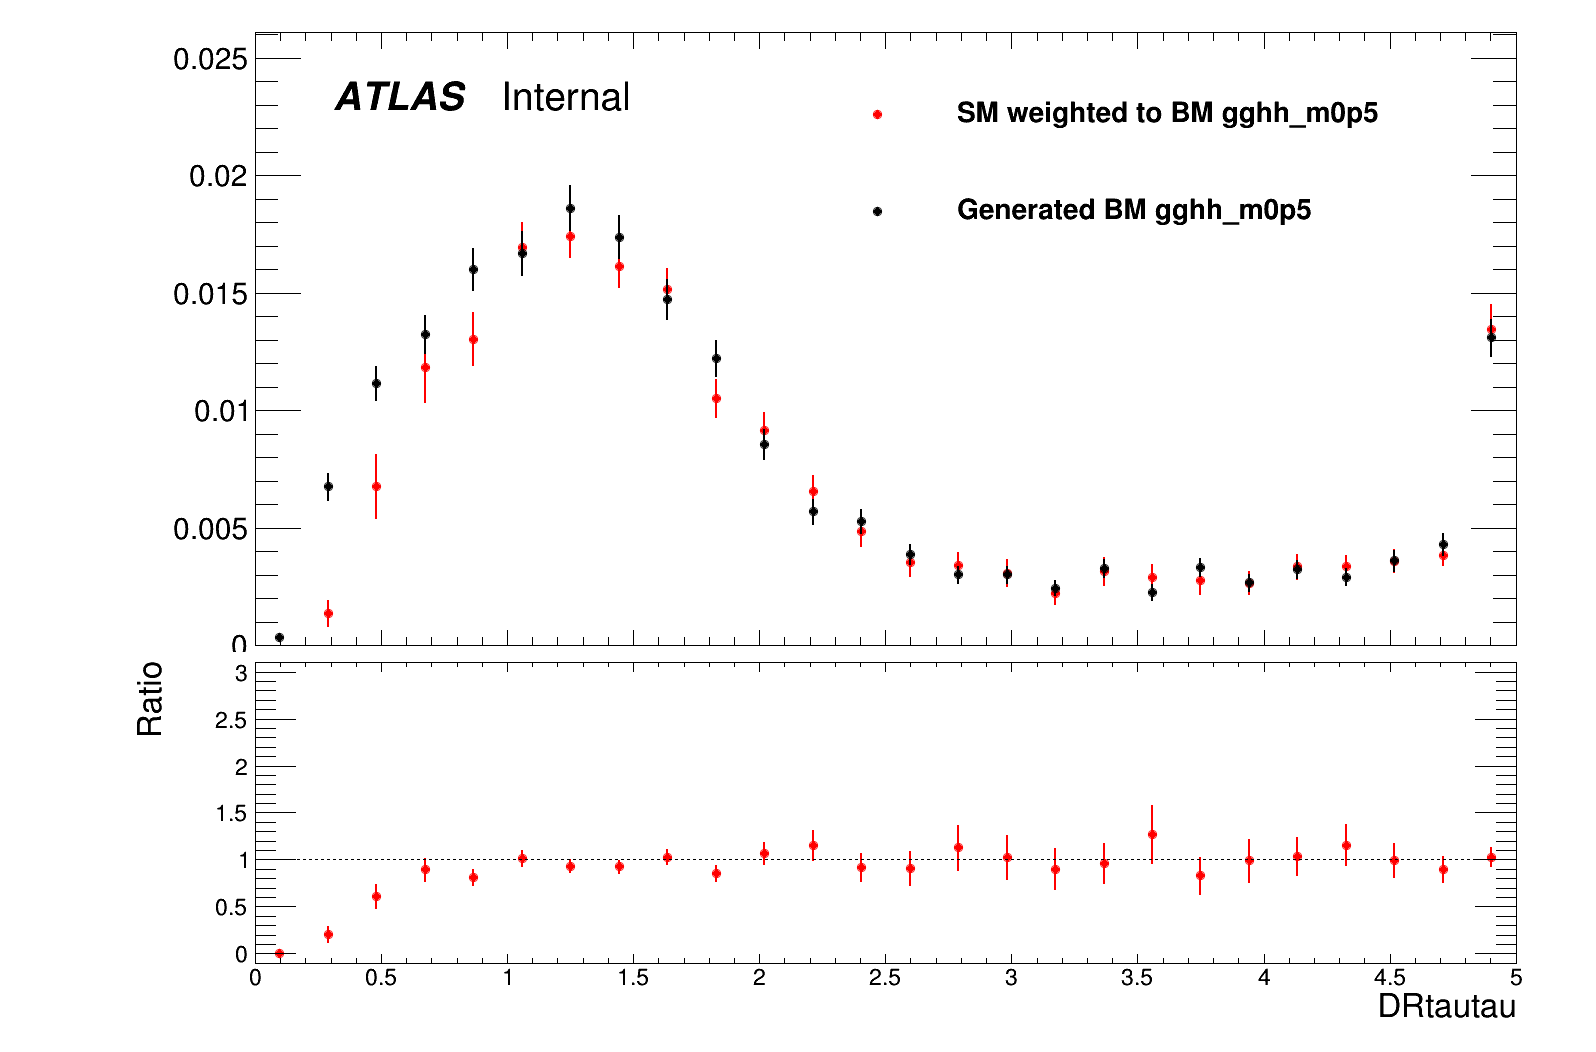
\includegraphics[width=.32\textwidth]{figures/Method_B_all_latest/BMgghh_m0p5h_DRtautau.png}
    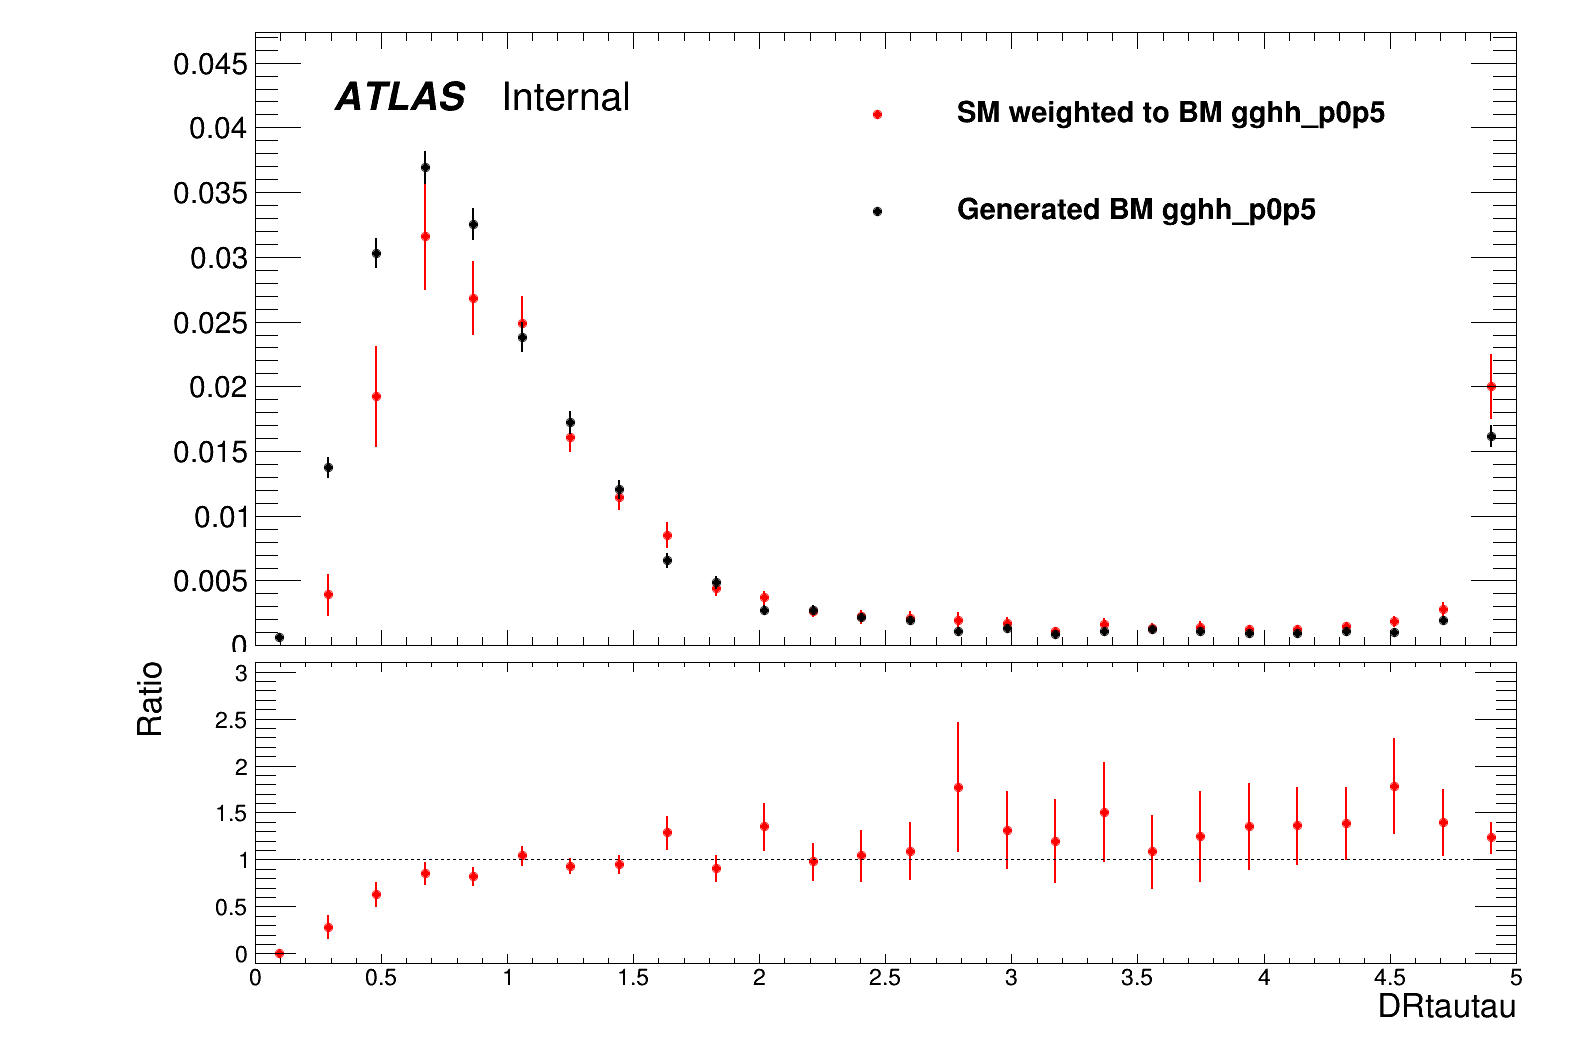
\includegraphics[width=.32\textwidth]{figures/Method_B_all_latest/BMgghh_p0p5h_DRtautau.png}
    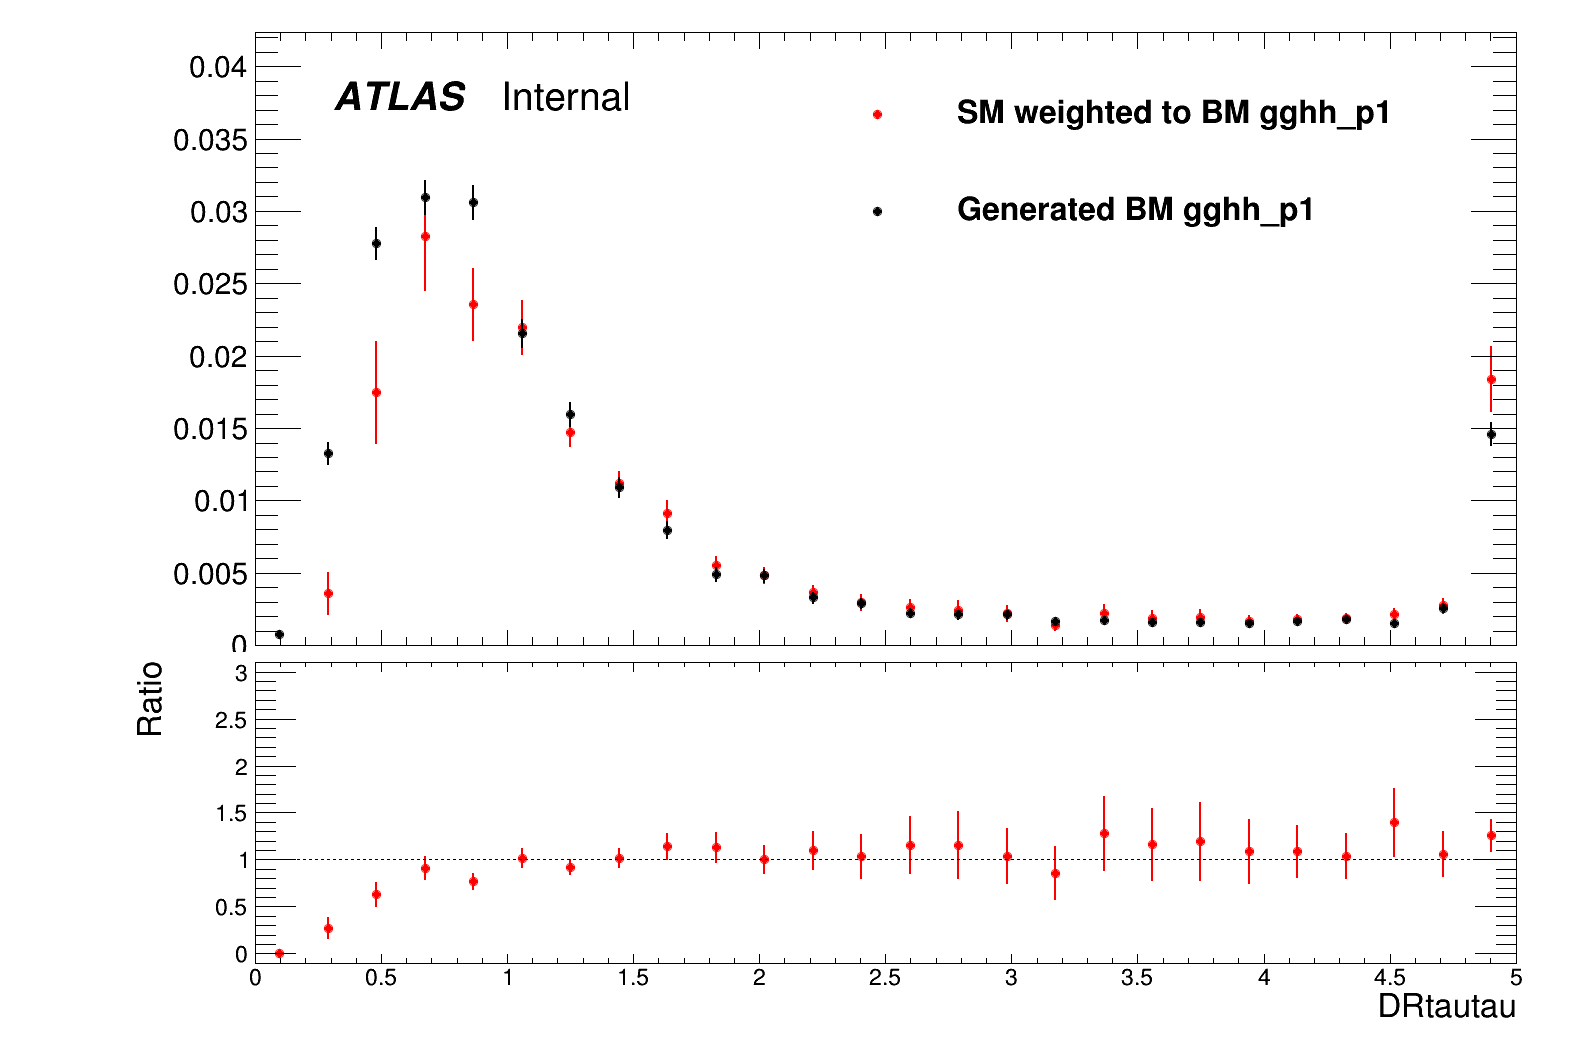
\includegraphics[width=.32\textwidth]{figures/Method_B_all_latest/BMgghh_p1h_DRtautau.png}
    $c_{ggHH} = -0.5$ \hspace{5em} $c_{ggHH} = 0.5$\hspace{5em} $c_{ggHH} = 1.0$
    \end{figure}


\end{frame}     

\begin{frame}
    \frametitle{Bkp: SLT $c_{ttHH}$ scan $\Delta R_{\tau\tau}$ shape: weighted SM vs generated BM}
\begin{figure}
    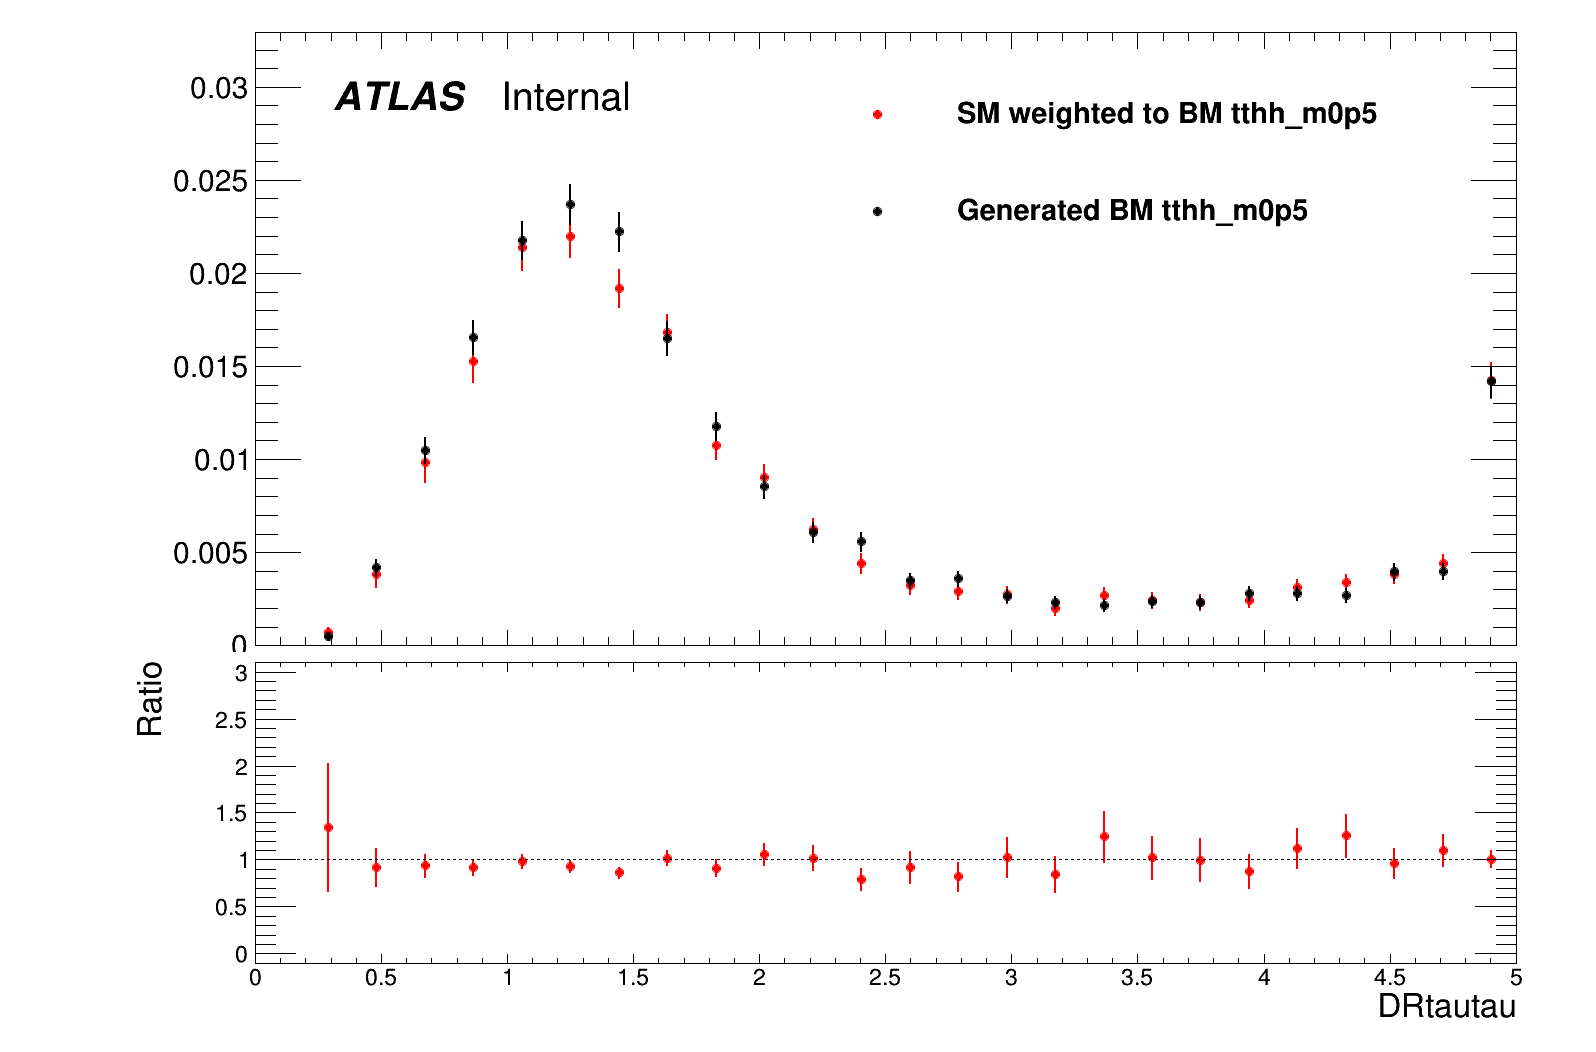
\includegraphics[width=.32\textwidth]{figures/Method_B_all_latest/BMtthh_m0p5h_DRtautau.png}
    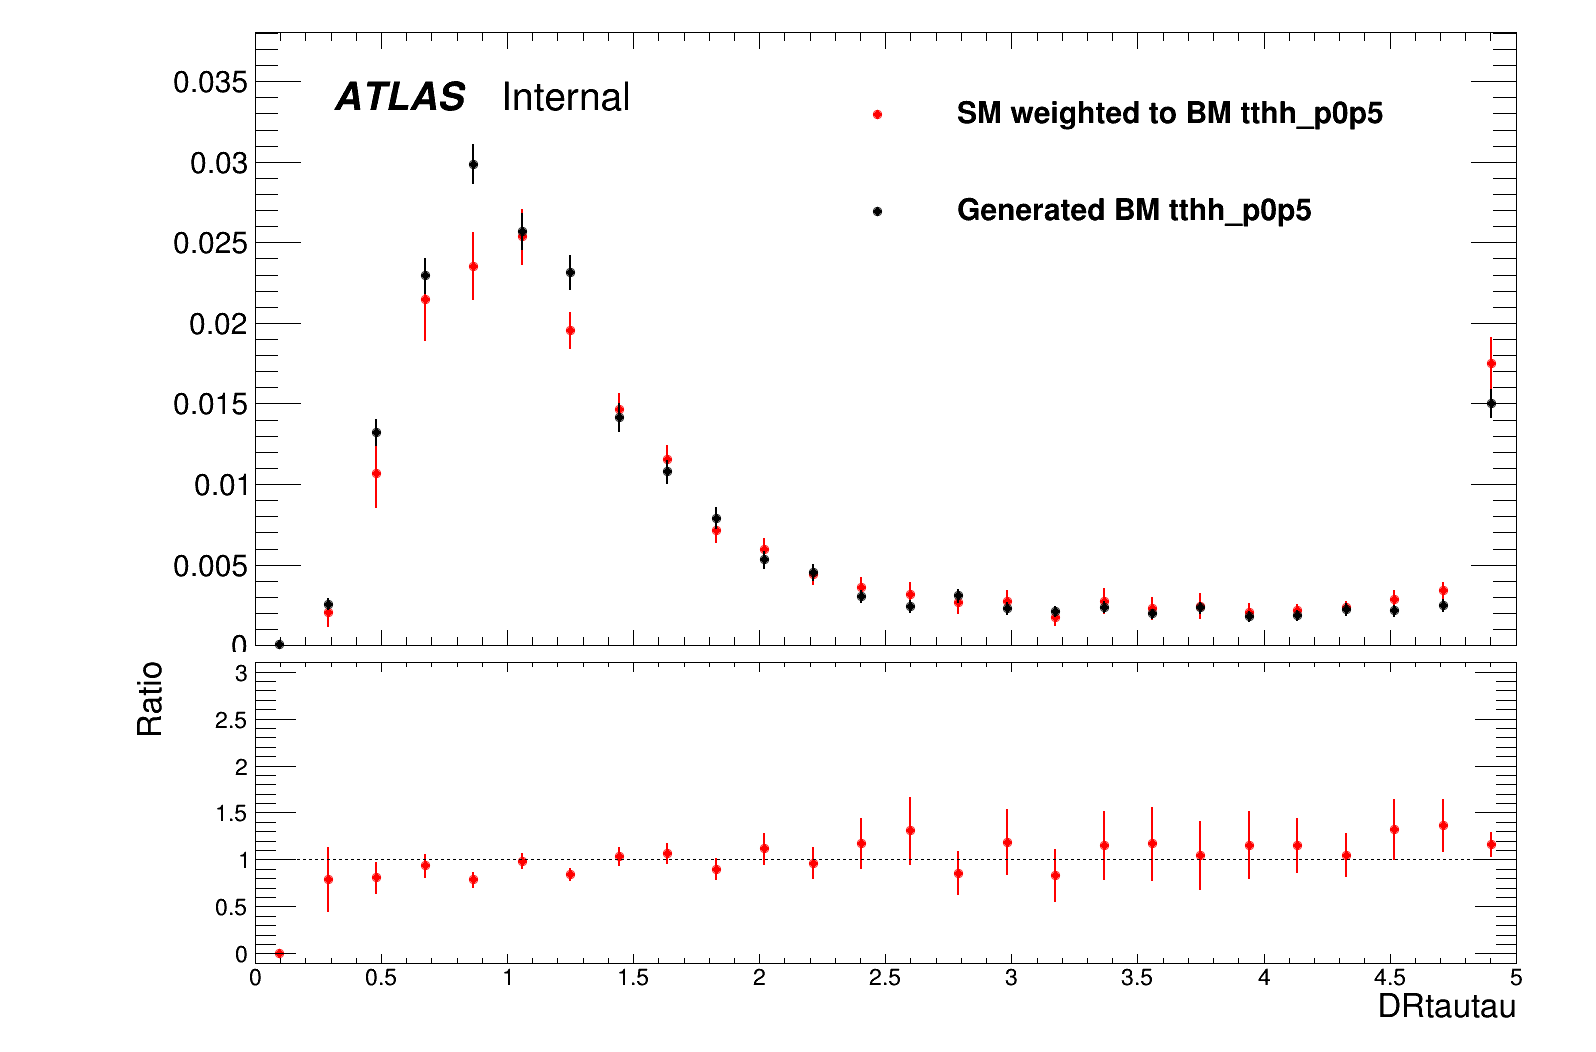
\includegraphics[width=.32\textwidth]{figures/Method_B_all_latest/BMtthh_p0p5h_DRtautau.png}
    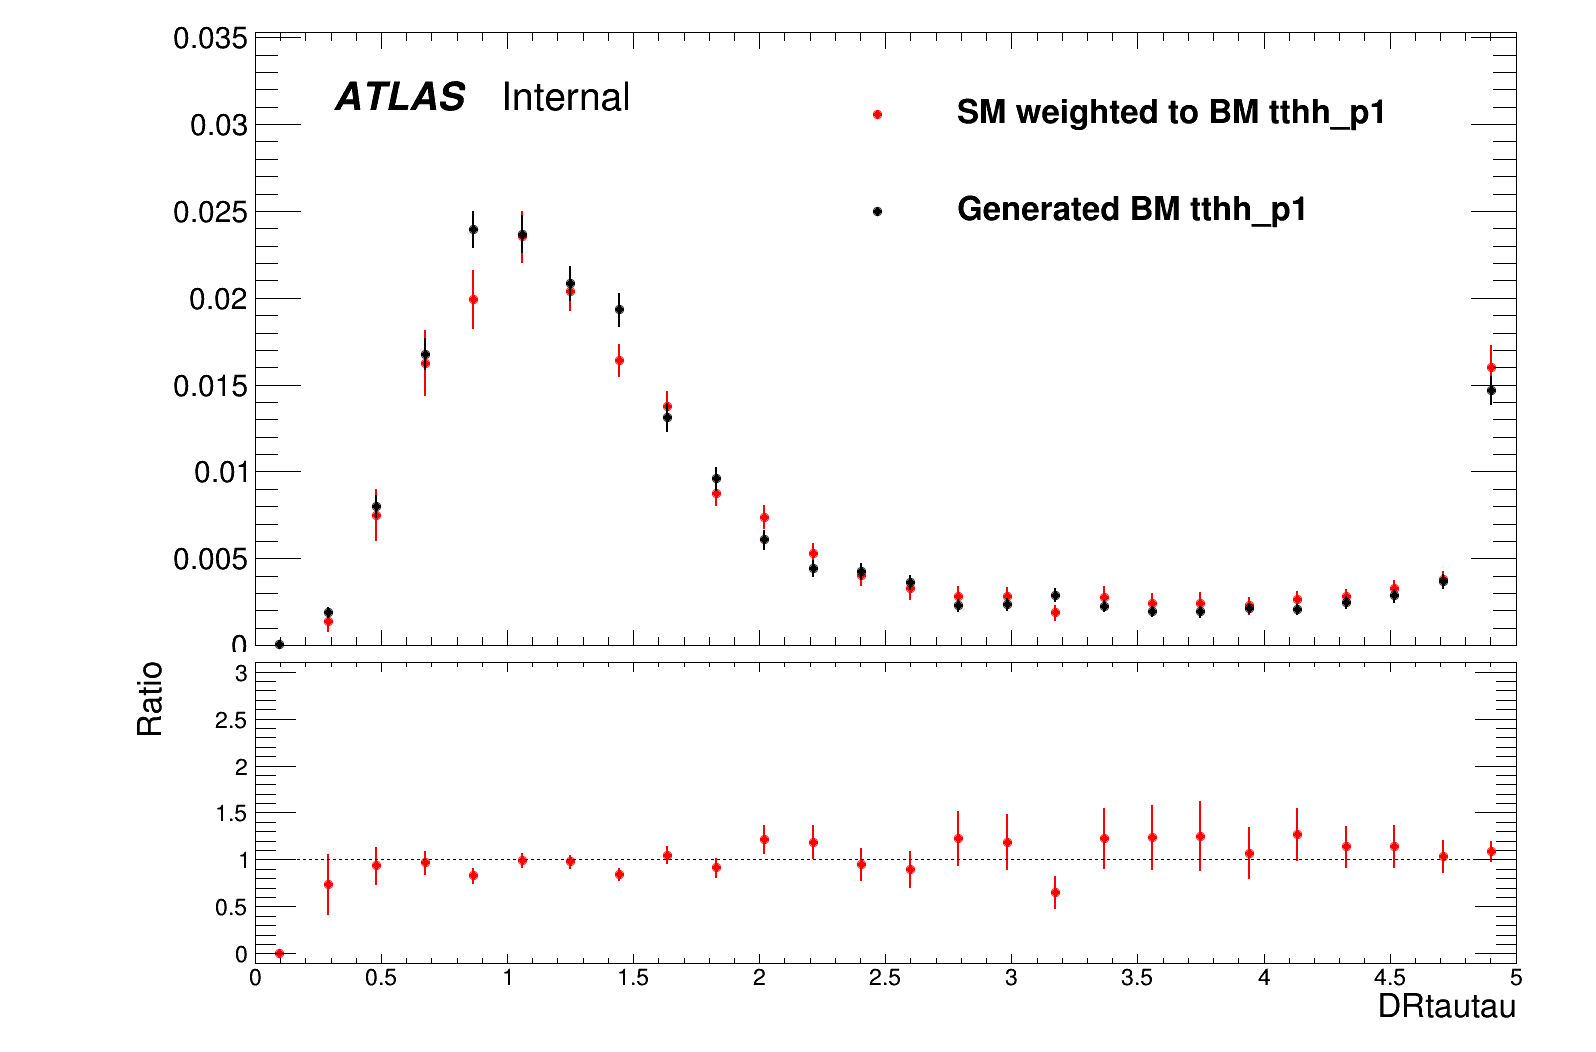
\includegraphics[width=.32\textwidth]{figures/Method_B_all_latest/BMtthh_p1h_DRtautau.png}
    $c_{ttHH} = -0.5$ \hspace{5em} $c_{ttHH} = 0.5$\hspace{5em} $c_{ttHH} = 1.0$    
\end{figure}

\end{frame}   




\begin{frame}
    \frametitle{Bkp: LTT BMs $\Delta R_{\tau\tau}$ shape: weighted SM vs generated BM}
\centering  
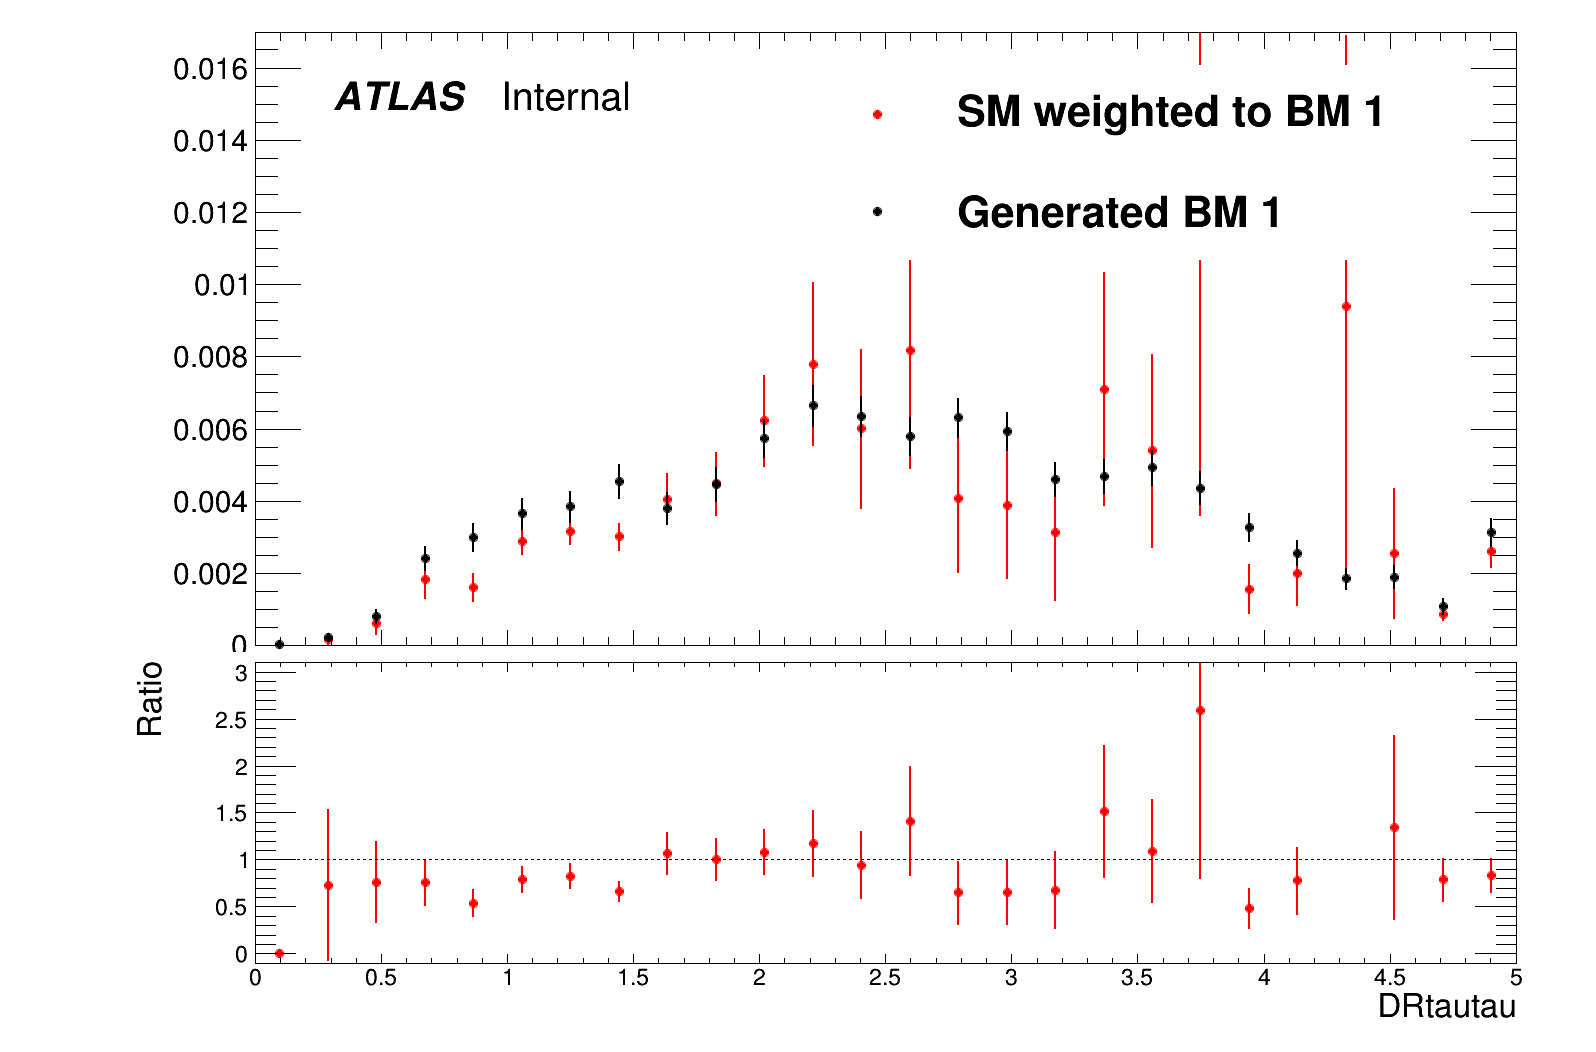
\includegraphics[width=.32\textwidth]{figures/Method_B_all_latest_LTT/BM1h_DRtautau.png}
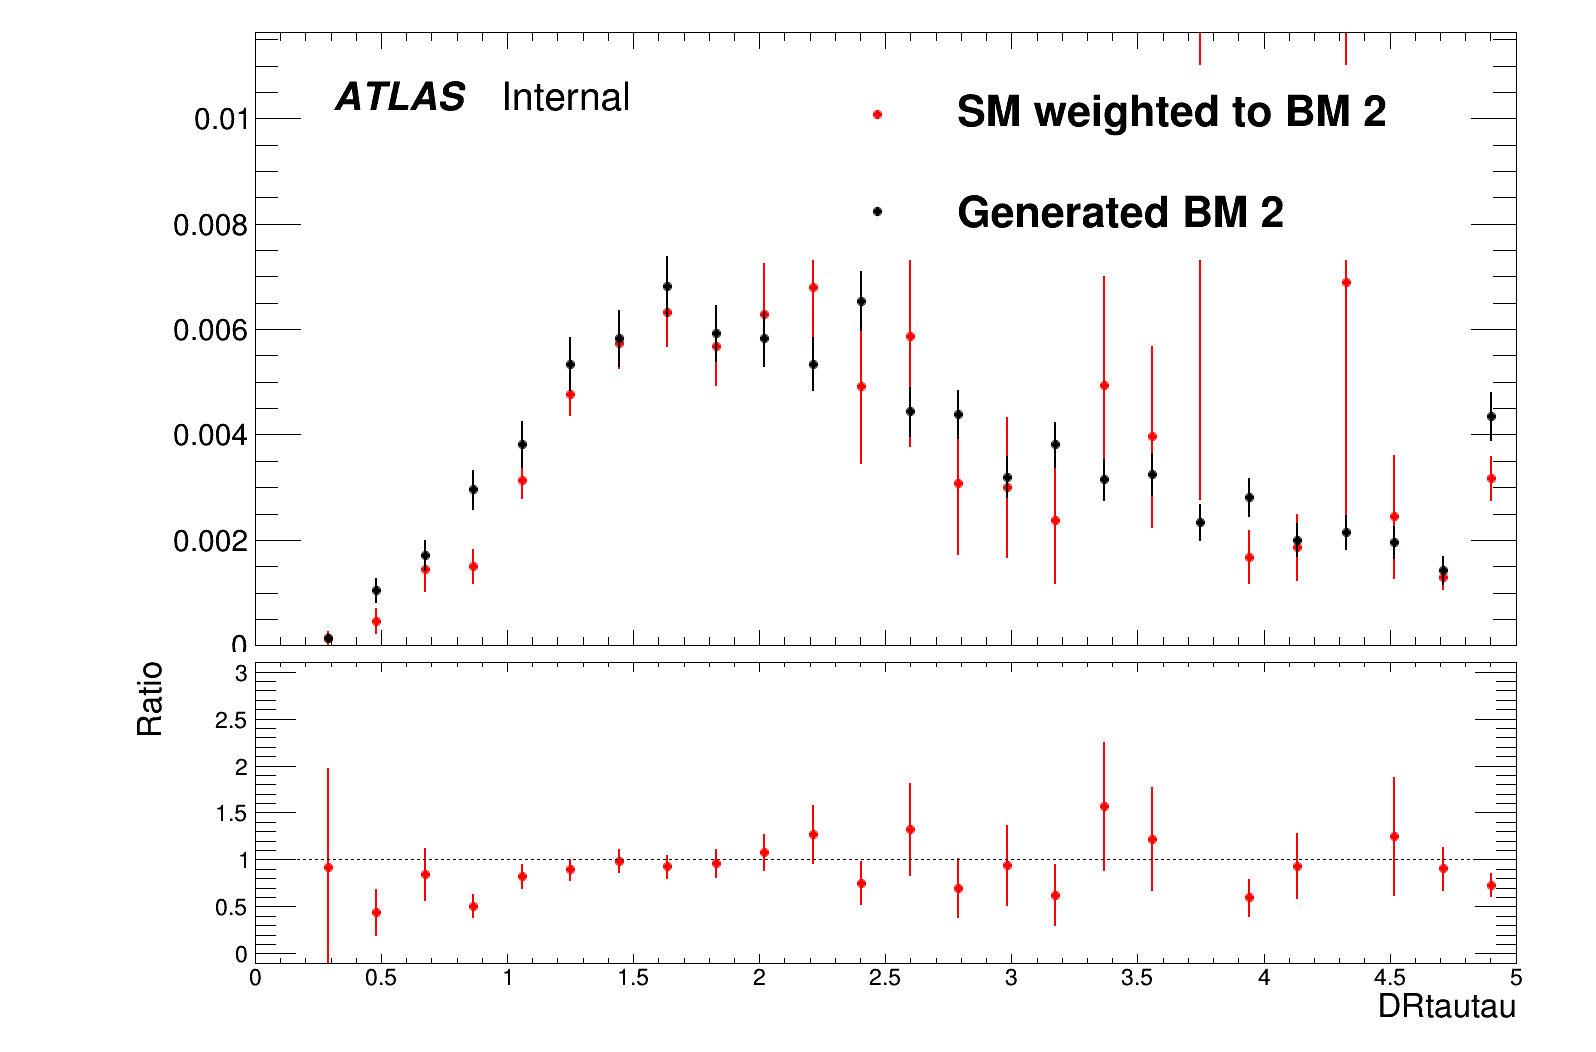
\includegraphics[width=.32\textwidth]{figures/Method_B_all_latest_LTT/BM2h_DRtautau.png}
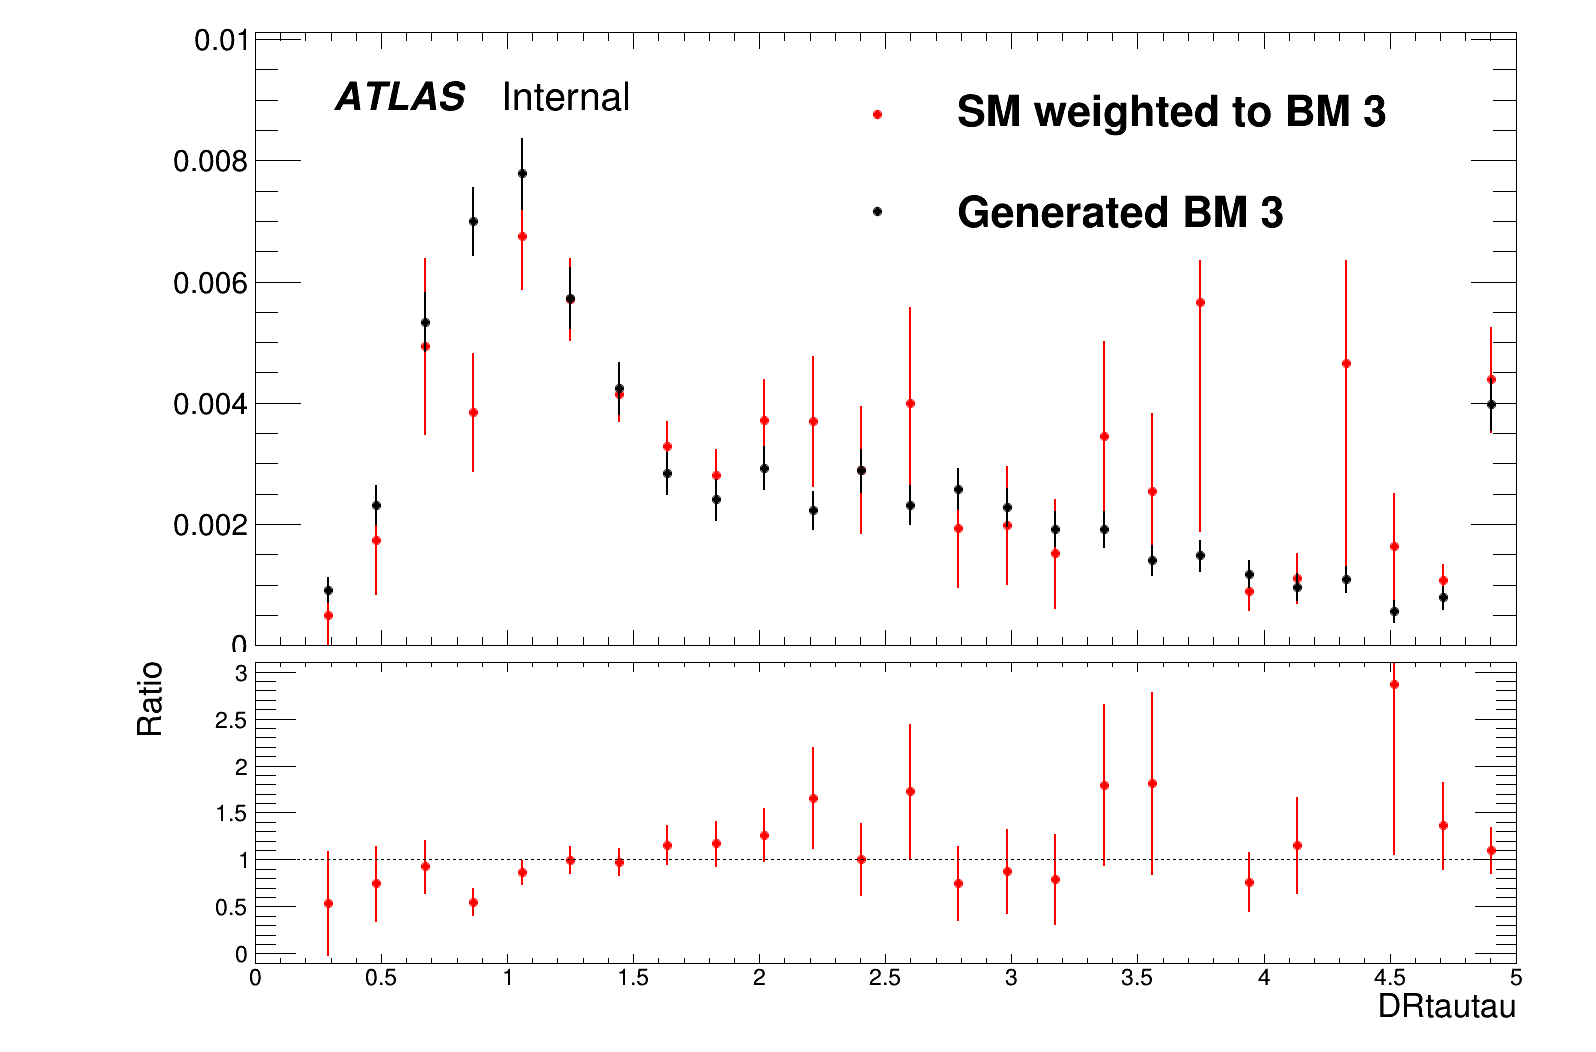
\includegraphics[width=.32\textwidth]{figures/Method_B_all_latest_LTT/BM3h_DRtautau.png}\\
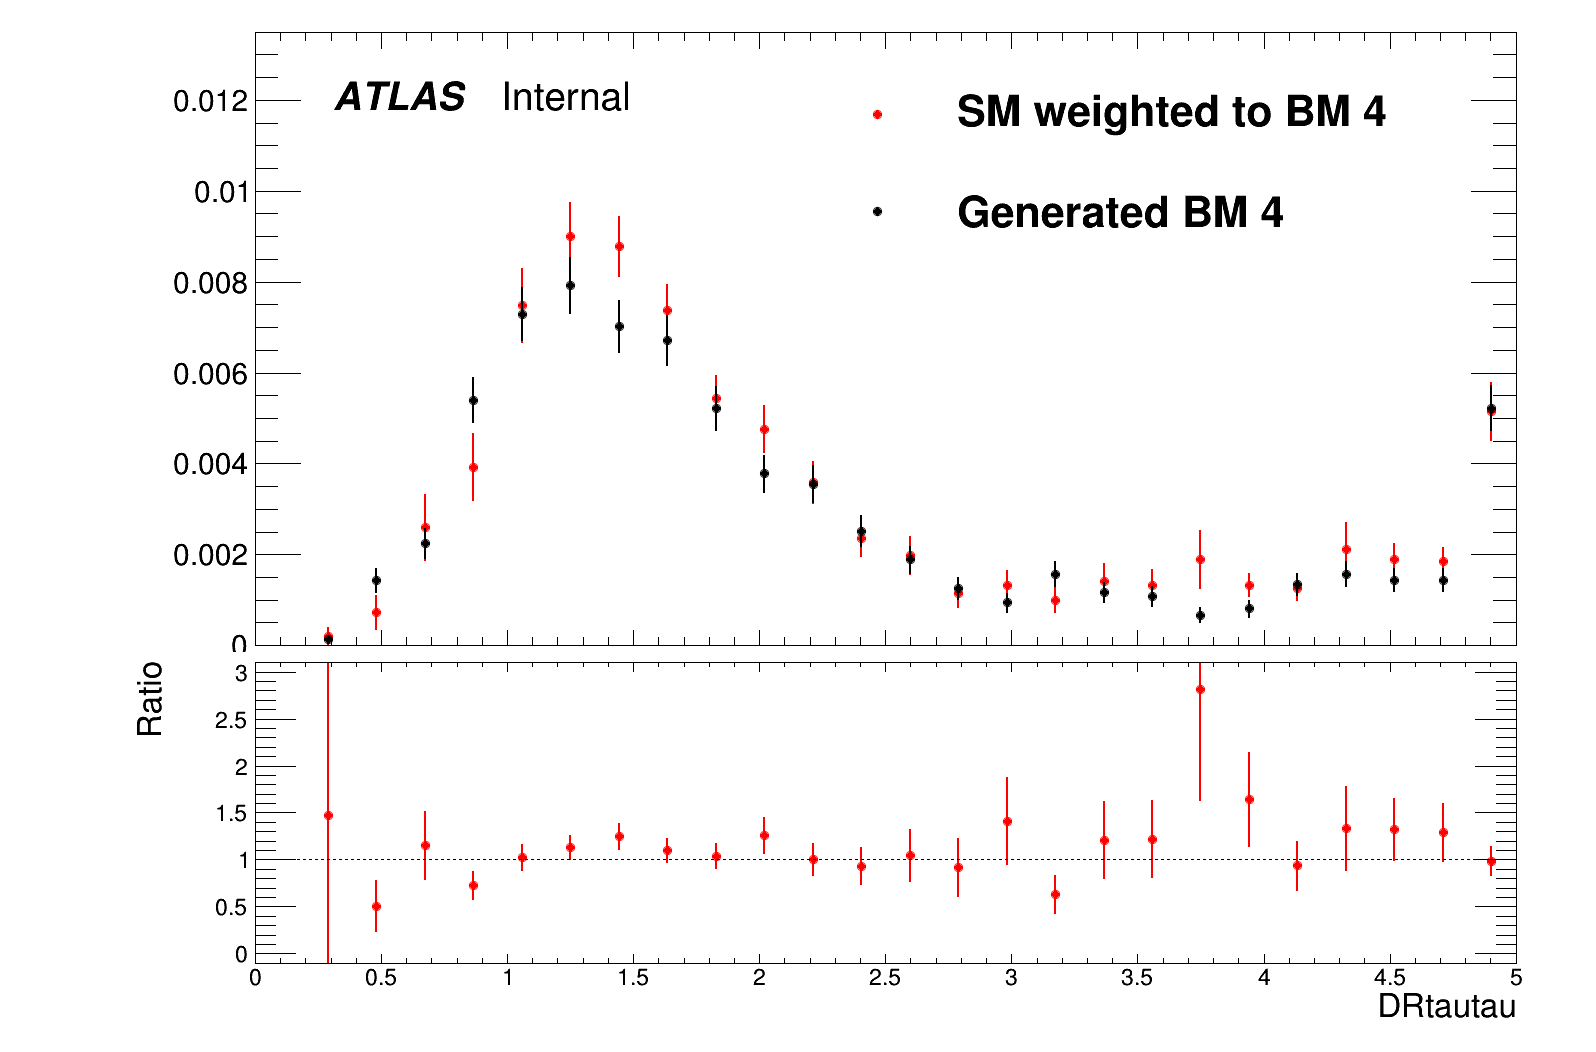
\includegraphics[width=.32\textwidth]{figures/Method_B_all_latest_LTT/BM4h_DRtautau.png}
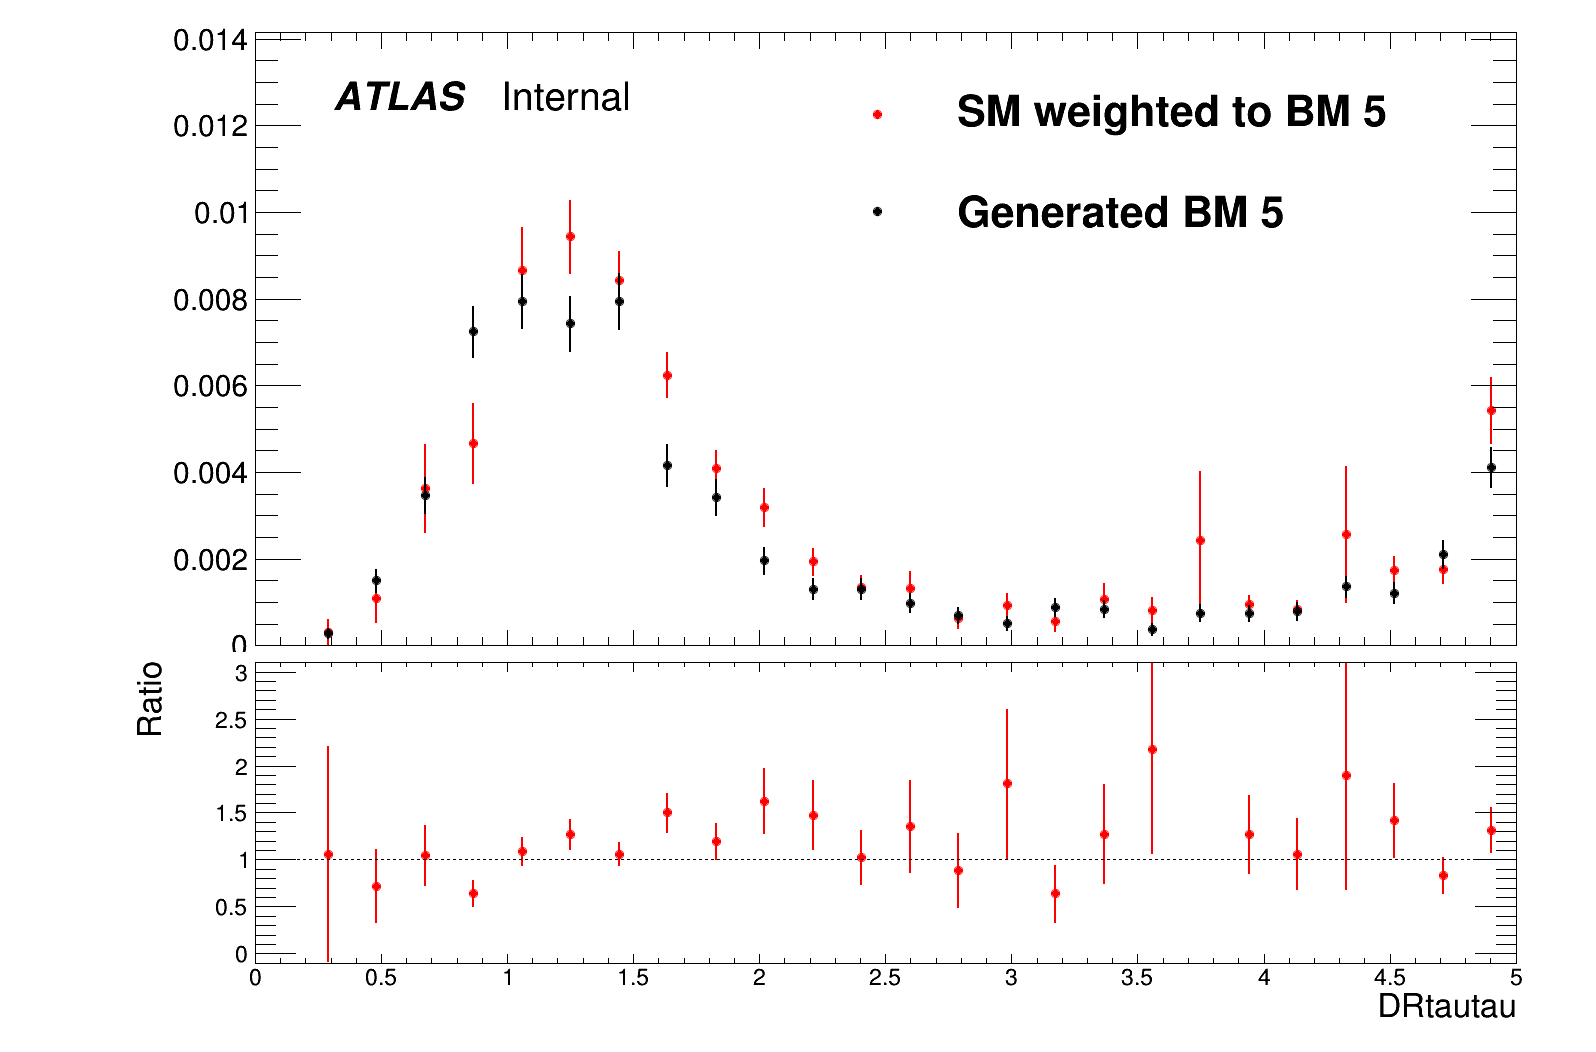
\includegraphics[width=.32\textwidth]{figures/Method_B_all_latest_LTT/BM5h_DRtautau.png}
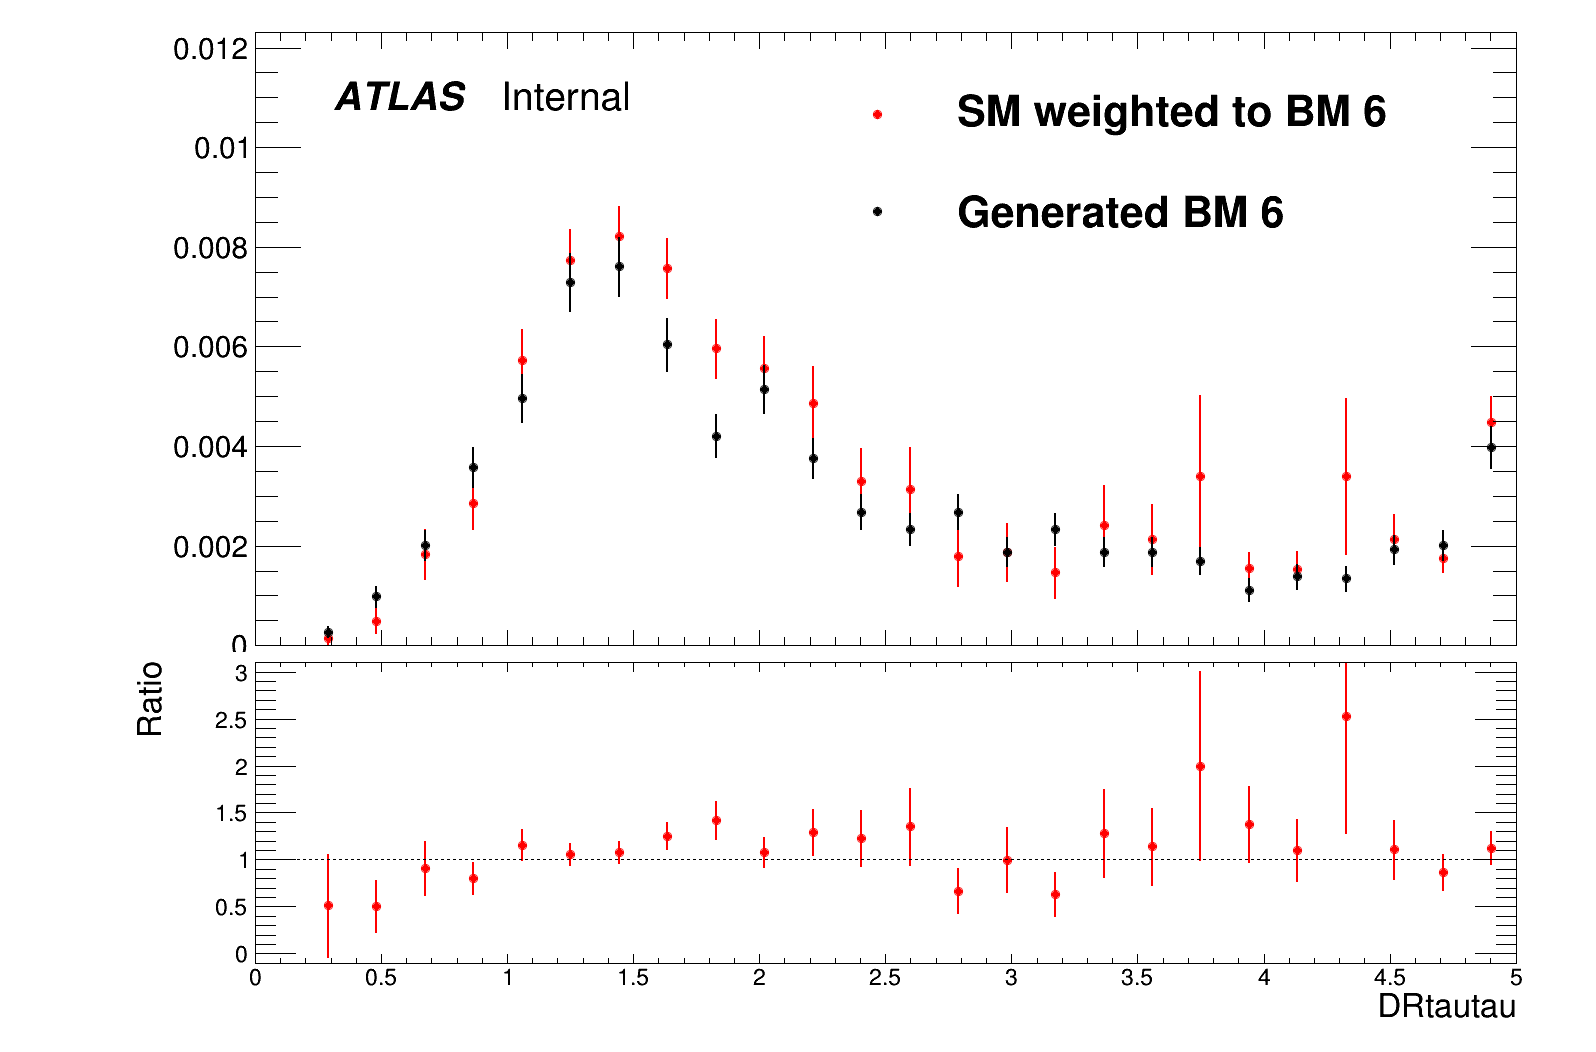
\includegraphics[width=.32\textwidth]{figures/Method_B_all_latest_LTT/BM6h_DRtautau.png}\\
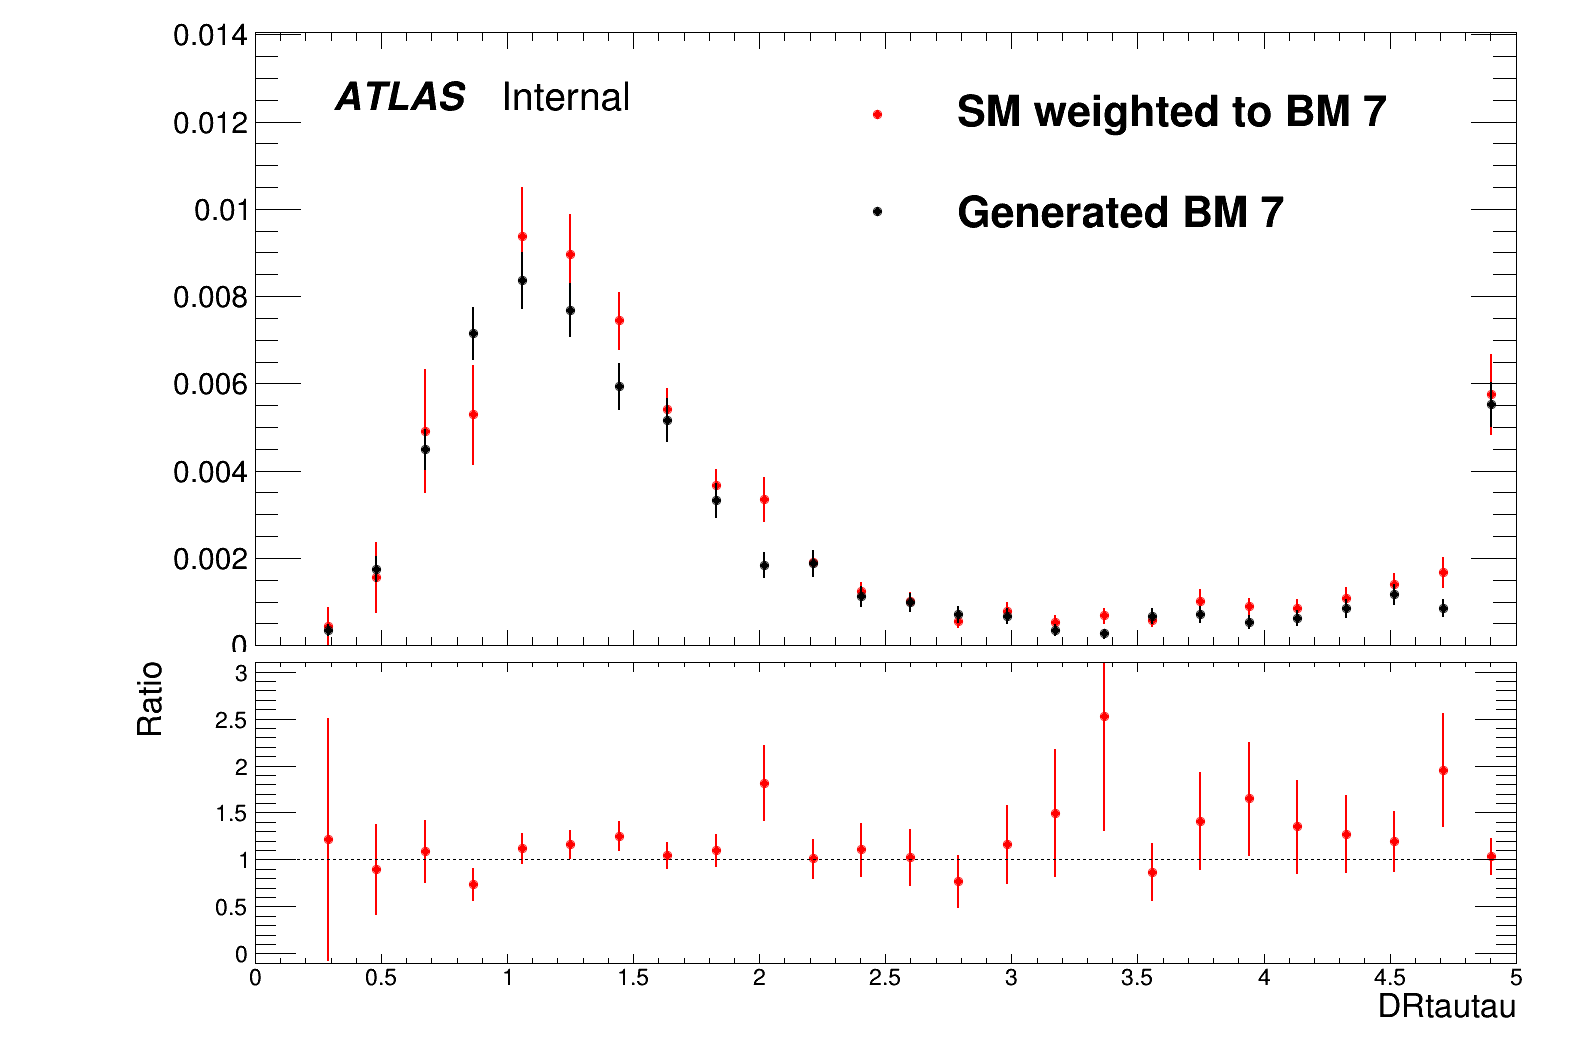
\includegraphics[width=.32\textwidth]{figures/Method_B_all_latest_LTT/BM7h_DRtautau.png}

\end{frame}


\begin{frame}
\frametitle{Bkp: LTT $c_{ggHH}$ scan $\Delta R_{\tau\tau}$ shape: weighted SM vs generated BM}

\begin{figure}
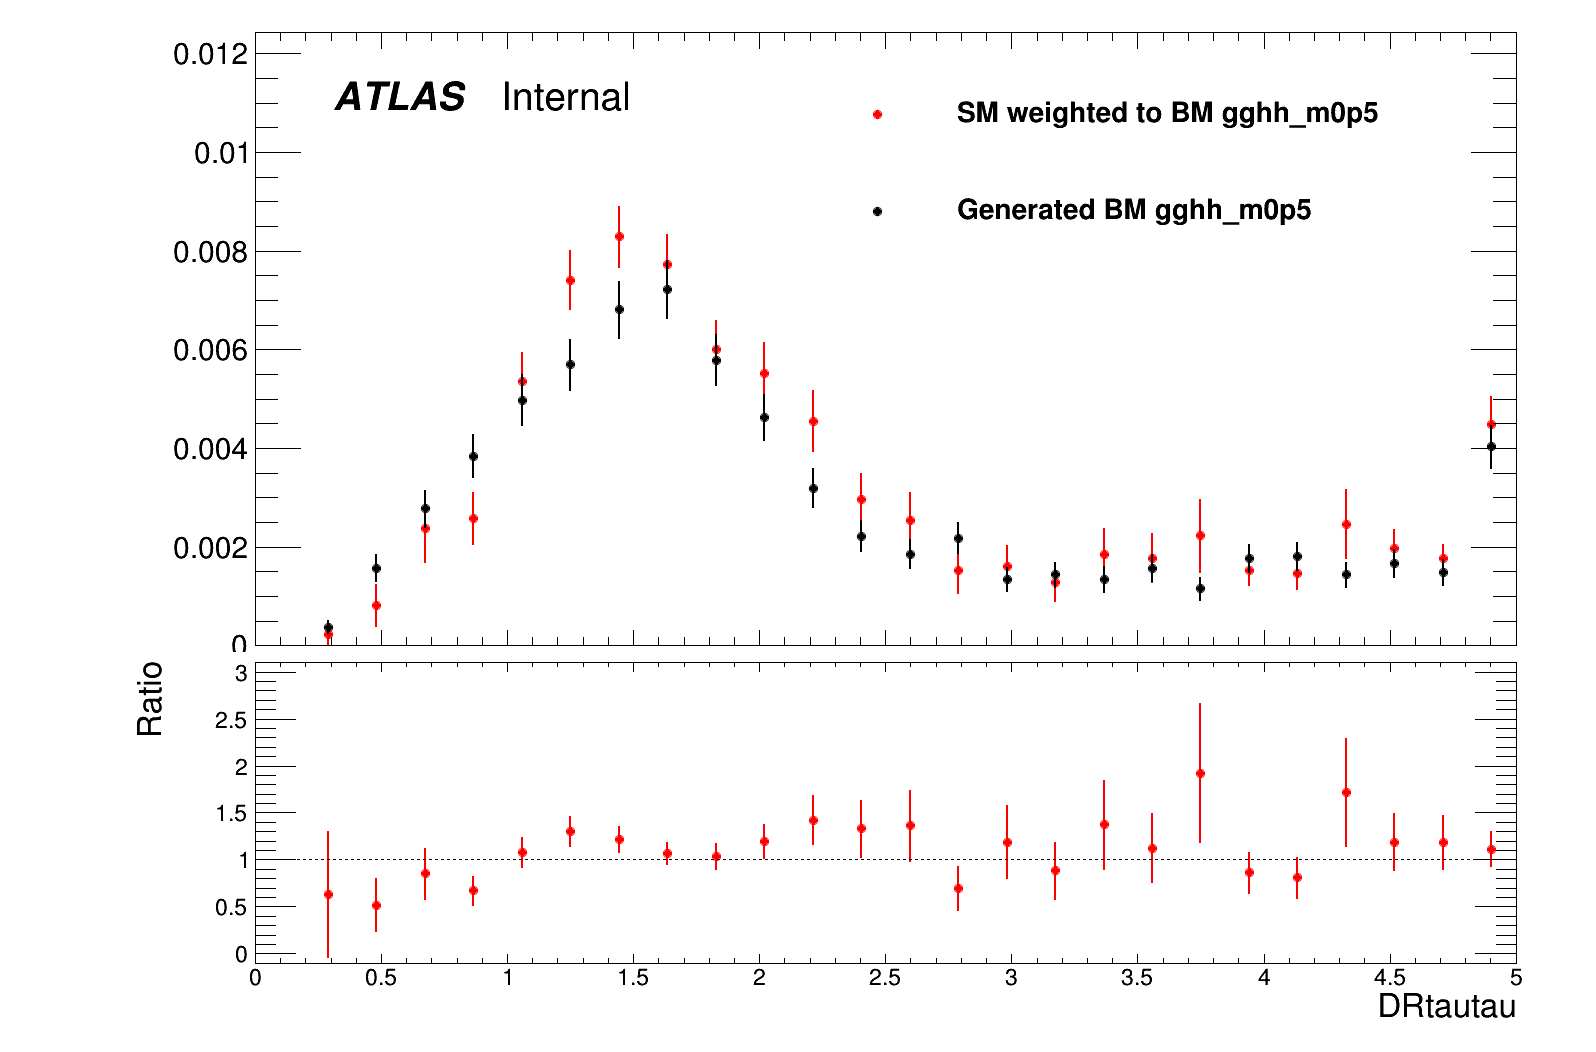
\includegraphics[width=.32\textwidth]{figures/Method_B_all_latest_LTT/BMgghh_m0p5h_DRtautau.png}
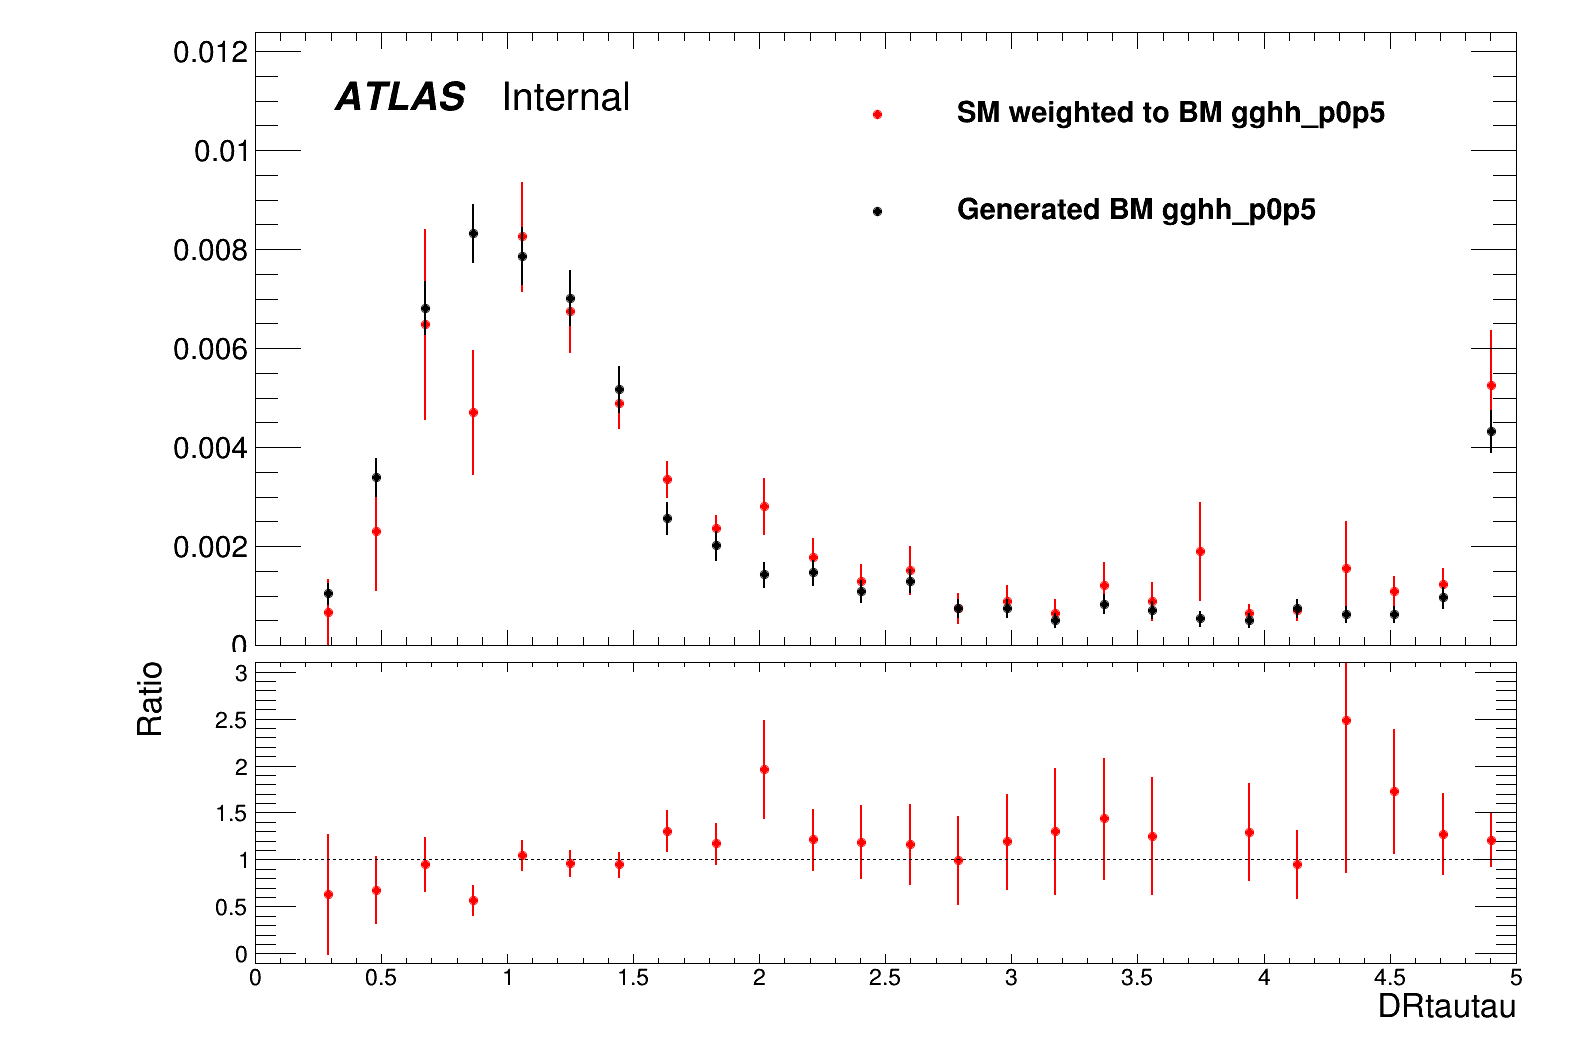
\includegraphics[width=.32\textwidth]{figures/Method_B_all_latest_LTT/BMgghh_p0p5h_DRtautau.png}
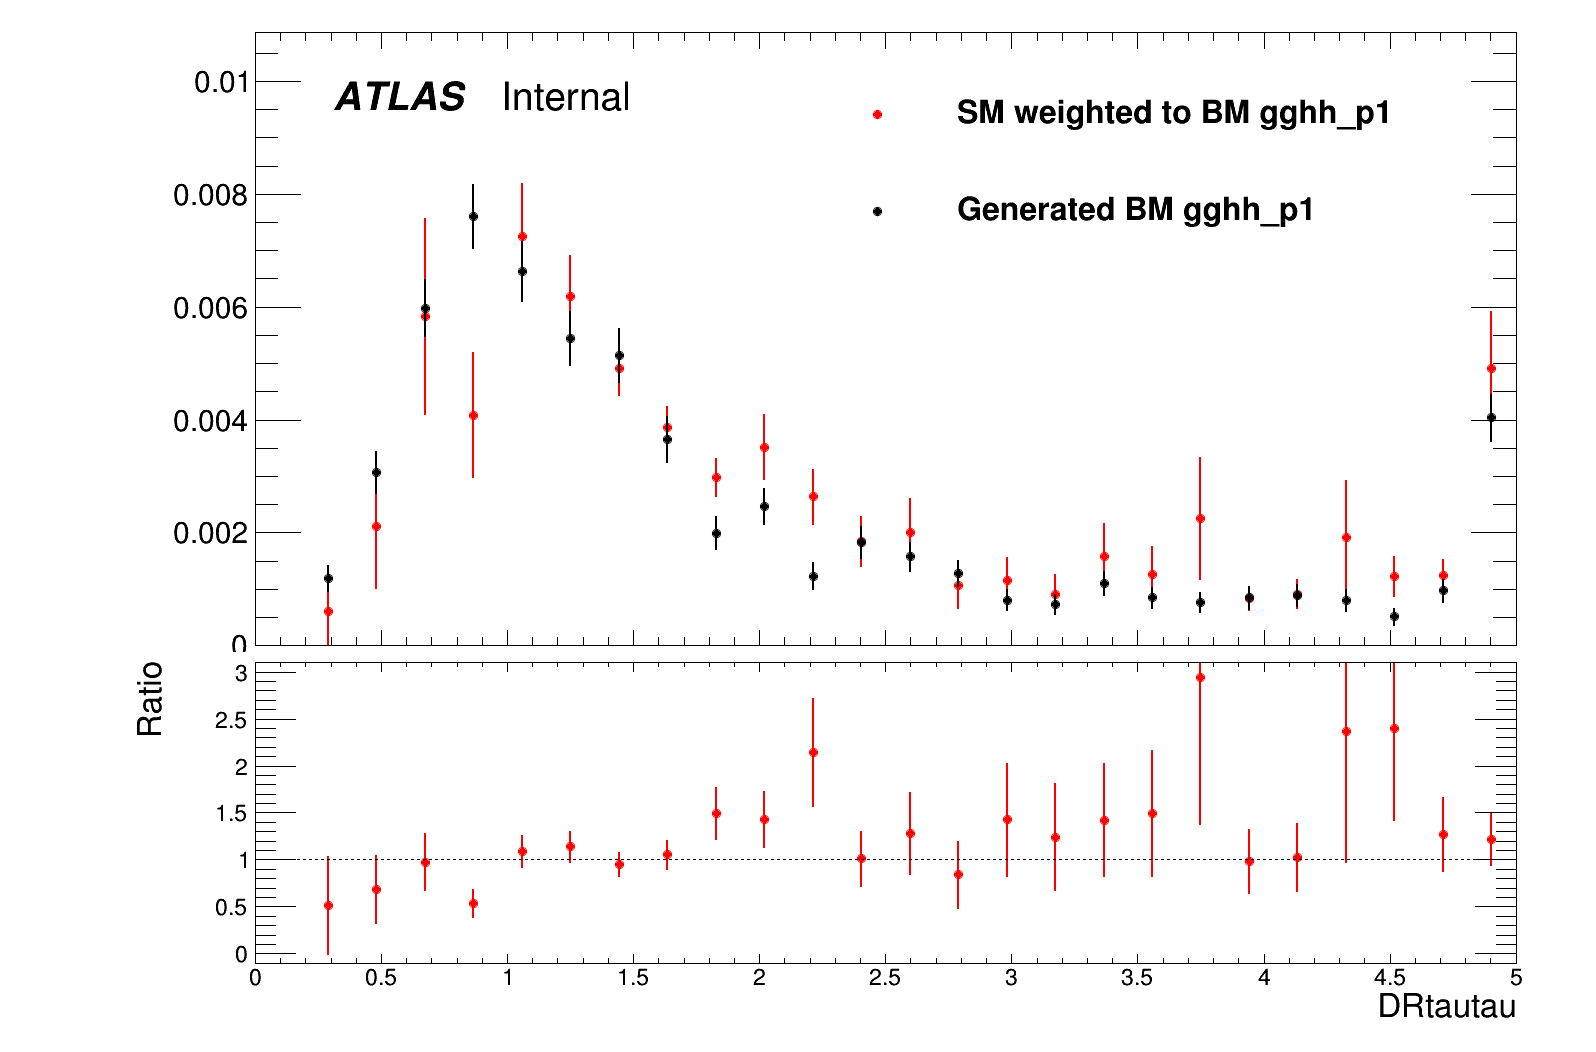
\includegraphics[width=.32\textwidth]{figures/Method_B_all_latest_LTT/BMgghh_p1h_DRtautau.png}
$c_{ggHH} = -0.5$ \hspace{5em} $c_{ggHH} = 0.5$\hspace{5em} $c_{ggHH} = 1.0$
\end{figure}


\end{frame}     

\begin{frame}
\frametitle{Bkp: LTT $c_{ttHH}$ scan $\Delta R_{\tau\tau}$ shape: weighted SM vs generated BM}
\begin{figure}
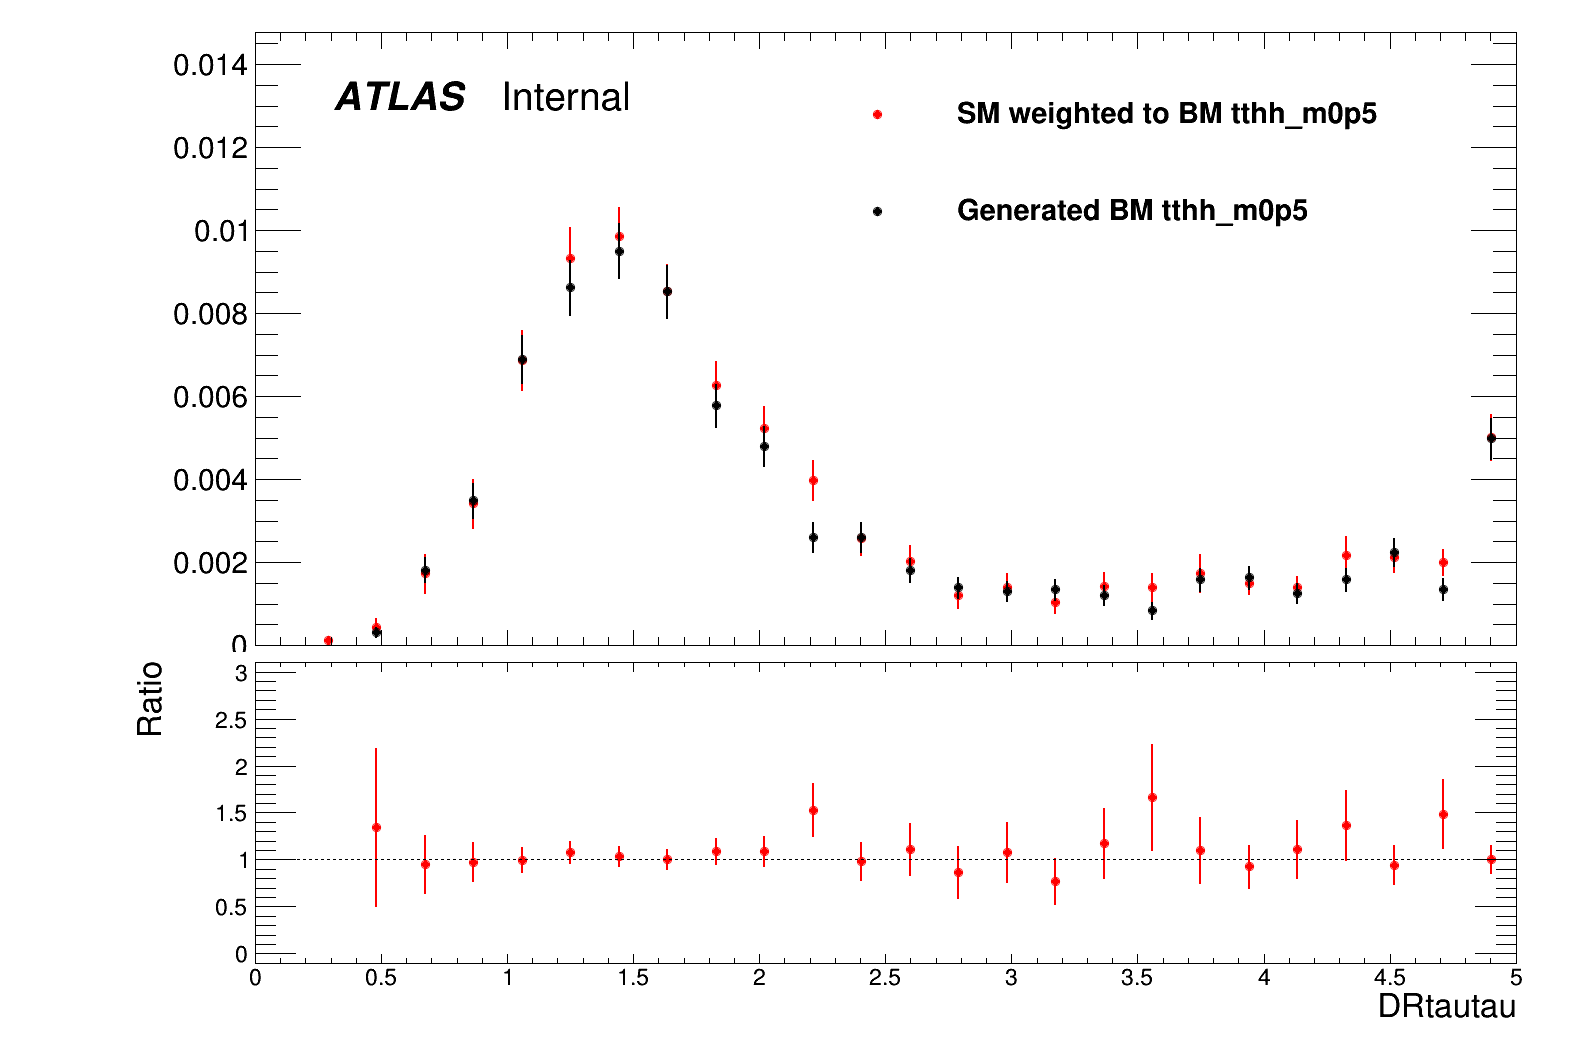
\includegraphics[width=.32\textwidth]{figures/Method_B_all_latest_LTT/BMtthh_m0p5h_DRtautau.png}
\includegraphics[width=.32\textwidth]{figures/Method_B_all_latest_LTT/BMtthh_p0p5h_DRtautau.png}
\includegraphics[width=.32\textwidth]{figures/Method_B_all_latest_LTT/BMtthh_p1h_DRtautau.png}
$c_{ttHH} = -0.5$ \hspace{5em} $c_{ttHH} = 0.5$\hspace{5em} $c_{ttHH} = 1.0$    
\end{figure}

\end{frame}   



\begin{frame}
    \frametitle{Bkp: SLT BMs $\Delta R_{bb}$ shape: weighted SM vs generated BM}
\centering  
\includegraphics[width=.32\textwidth]{figures/Method_B_all_latest/BM1h_DRbb.png}
\includegraphics[width=.32\textwidth]{figures/Method_B_all_latest/BM2h_DRbb.png}
\includegraphics[width=.32\textwidth]{figures/Method_B_all_latest/BM3h_DRbb.png}\\
\includegraphics[width=.32\textwidth]{figures/Method_B_all_latest/BM4h_DRbb.png}
\includegraphics[width=.32\textwidth]{figures/Method_B_all_latest/BM5h_DRbb.png}
\includegraphics[width=.32\textwidth]{figures/Method_B_all_latest/BM6h_DRbb.png}\\
\includegraphics[width=.32\textwidth]{figures/Method_B_all_latest/BM7h_DRbb.png}

\end{frame}

\begin{frame}
    \frametitle{Bkp: SLT $c_{ggHH}$ scan $\Delta R_{bb}$ shape: weighted SM vs generated BM}

    \begin{figure}
    \includegraphics[width=.32\textwidth]{figures/Method_B_all_latest/BMgghh_m0p5h_DRbb.png}
    \includegraphics[width=.32\textwidth]{figures/Method_B_all_latest/BMgghh_p0p5h_DRbb.png}
    \includegraphics[width=.32\textwidth]{figures/Method_B_all_latest/BMgghh_p1h_DRbb.png}
    $c_{ggHH} = -0.5$ \hspace{5em} $c_{ggHH} = 0.5$\hspace{5em} $c_{ggHH} = 1.0$
    \end{figure}


\end{frame}     

\begin{frame}
    \frametitle{Bkp: SLT $c_{ttHH}$ scan $\Delta R_{bb}$ shape: weighted SM vs generated BM}
\begin{figure}
    \includegraphics[width=.32\textwidth]{figures/Method_B_all_latest/BMtthh_m0p5h_DRbb.png}
    \includegraphics[width=.32\textwidth]{figures/Method_B_all_latest/BMtthh_p0p5h_DRbb.png}
    \includegraphics[width=.32\textwidth]{figures/Method_B_all_latest/BMtthh_p1h_DRbb.png}
    $c_{ttHH} = -0.5$ \hspace{5em} $c_{ttHH} = 0.5$\hspace{5em} $c_{ttHH} = 1.0$    
\end{figure}

\end{frame}   




\begin{frame}
    \frametitle{Bkp: LTT BMs $\Delta R_{bb}$ shape: weighted SM vs generated BM}
\centering  
\includegraphics[width=.32\textwidth]{figures/Method_B_all_latest_LTT/BM1h_DRbb.png}
\includegraphics[width=.32\textwidth]{figures/Method_B_all_latest_LTT/BM2h_DRbb.png}
\includegraphics[width=.32\textwidth]{figures/Method_B_all_latest_LTT/BM3h_DRbb.png}\\
\includegraphics[width=.32\textwidth]{figures/Method_B_all_latest_LTT/BM4h_DRbb.png}
\includegraphics[width=.32\textwidth]{figures/Method_B_all_latest_LTT/BM5h_DRbb.png}
\includegraphics[width=.32\textwidth]{figures/Method_B_all_latest_LTT/BM6h_DRbb.png}\\
\includegraphics[width=.32\textwidth]{figures/Method_B_all_latest_LTT/BM7h_DRbb.png}

\end{frame}


\begin{frame}
\frametitle{Bkp: LTT $c_{ggHH}$ scan $\Delta R_{bb}$ shape: weighted SM vs generated BM}

\begin{figure}
\includegraphics[width=.32\textwidth]{figures/Method_B_all_latest_LTT/BMgghh_m0p5h_DRbb.png}
\includegraphics[width=.32\textwidth]{figures/Method_B_all_latest_LTT/BMgghh_p0p5h_DRbb.png}
\includegraphics[width=.32\textwidth]{figures/Method_B_all_latest_LTT/BMgghh_p1h_DRbb.png}
$c_{ggHH} = -0.5$ \hspace{5em} $c_{ggHH} = 0.5$\hspace{5em} $c_{ggHH} = 1.0$
\end{figure}


\end{frame}     

\begin{frame}
\frametitle{Bkp: LTT $c_{ttHH}$ scan $\Delta R_{bb}$ shape: weighted SM vs generated BM}
\begin{figure}
\includegraphics[width=.32\textwidth]{figures/Method_B_all_latest_LTT/BMtthh_m0p5h_DRbb.png}
\includegraphics[width=.32\textwidth]{figures/Method_B_all_latest_LTT/BMtthh_p0p5h_DRbb.png}
\includegraphics[width=.32\textwidth]{figures/Method_B_all_latest_LTT/BMtthh_p1h_DRbb.png}
$c_{ttHH} = -0.5$ \hspace{5em} $c_{ttHH} = 0.5$\hspace{5em} $c_{ttHH} = 1.0$    
\end{figure}

\end{frame}   



\begin{frame}
    \frametitle{Bkp: SLT BMs $m_{bb}$ shape: weighted SM vs generated BM}
\centering  
\includegraphics[width=.32\textwidth]{figures/Method_B_all_latest/BM1h_mbb.png}
\includegraphics[width=.32\textwidth]{figures/Method_B_all_latest/BM2h_mbb.png}
\includegraphics[width=.32\textwidth]{figures/Method_B_all_latest/BM3h_mbb.png}\\
\includegraphics[width=.32\textwidth]{figures/Method_B_all_latest/BM4h_mbb.png}
\includegraphics[width=.32\textwidth]{figures/Method_B_all_latest/BM5h_mbb.png}
\includegraphics[width=.32\textwidth]{figures/Method_B_all_latest/BM6h_mbb.png}\\
\includegraphics[width=.32\textwidth]{figures/Method_B_all_latest/BM7h_mbb.png}

\end{frame}

\begin{frame}
    \frametitle{Bkp: SLT $c_{ggHH}$ scan $m_{bb}$ shape: weighted SM vs generated BM}

    \begin{figure}
    \includegraphics[width=.32\textwidth]{figures/Method_B_all_latest/BMgghh_m0p5h_mbb.png}
    \includegraphics[width=.32\textwidth]{figures/Method_B_all_latest/BMgghh_p0p5h_mbb.png}
    \includegraphics[width=.32\textwidth]{figures/Method_B_all_latest/BMgghh_p1h_mbb.png}
    $c_{ggHH} = -0.5$ \hspace{5em} $c_{ggHH} = 0.5$\hspace{5em} $c_{ggHH} = 1.0$
    \end{figure}


\end{frame}     

\begin{frame}
    \frametitle{Bkp: SLT $c_{ttHH}$ scan $m_{bb}$ shape: weighted SM vs generated BM}
\begin{figure}
    \includegraphics[width=.32\textwidth]{figures/Method_B_all_latest/BMtthh_m0p5h_mbb.png}
    \includegraphics[width=.32\textwidth]{figures/Method_B_all_latest/BMtthh_p0p5h_mbb.png}
    \includegraphics[width=.32\textwidth]{figures/Method_B_all_latest/BMtthh_p1h_mbb.png}
    $c_{ttHH} = -0.5$ \hspace{5em} $c_{ttHH} = 0.5$\hspace{5em} $c_{ttHH} = 1.0$    
\end{figure}

\end{frame}   




\begin{frame}
    \frametitle{Bkp: LTT BMs $m_{bb}$ shape: weighted SM vs generated BM}
\centering  
\includegraphics[width=.32\textwidth]{figures/Method_B_all_latest_LTT/BM1h_mbb.png}
\includegraphics[width=.32\textwidth]{figures/Method_B_all_latest_LTT/BM2h_mbb.png}
\includegraphics[width=.32\textwidth]{figures/Method_B_all_latest_LTT/BM3h_mbb.png}\\
\includegraphics[width=.32\textwidth]{figures/Method_B_all_latest_LTT/BM4h_mbb.png}
\includegraphics[width=.32\textwidth]{figures/Method_B_all_latest_LTT/BM5h_mbb.png}
\includegraphics[width=.32\textwidth]{figures/Method_B_all_latest_LTT/BM6h_mbb.png}\\
\includegraphics[width=.32\textwidth]{figures/Method_B_all_latest_LTT/BM7h_mbb.png}

\end{frame}


\begin{frame}
\frametitle{Bkp: LTT $c_{ggHH}$ scan $m_{bb}$ shape: weighted SM vs generated BM}

\begin{figure}
\includegraphics[width=.32\textwidth]{figures/Method_B_all_latest_LTT/BMgghh_m0p5h_mbb.png}
\includegraphics[width=.32\textwidth]{figures/Method_B_all_latest_LTT/BMgghh_p0p5h_mbb.png}
\includegraphics[width=.32\textwidth]{figures/Method_B_all_latest_LTT/BMgghh_p1h_mbb.png}
$c_{ggHH} = -0.5$ \hspace{5em} $c_{ggHH} = 0.5$\hspace{5em} $c_{ggHH} = 1.0$
\end{figure}


\end{frame}     

\begin{frame}
\frametitle{Bkp: LTT $c_{ttHH}$ scan $m_{bb}$ shape: weighted SM vs generated BM}
\begin{figure}
\includegraphics[width=.32\textwidth]{figures/Method_B_all_latest_LTT/BMtthh_m0p5h_mbb.png}
\includegraphics[width=.32\textwidth]{figures/Method_B_all_latest_LTT/BMtthh_p0p5h_mbb.png}
\includegraphics[width=.32\textwidth]{figures/Method_B_all_latest_LTT/BMtthh_p1h_mbb.png}
$c_{ttHH} = -0.5$ \hspace{5em} $c_{ttHH} = 0.5$\hspace{5em} $c_{ttHH} = 1.0$    
\end{figure}

\end{frame}   



















\end{document}